\documentclass[10pt]{article}
\usepackage[a4paper, total={6in, 8in}]{geometry}
\usepackage[utf8]{inputenc}
\usepackage{latexsym}
\setlength{\parskip}{1em}                   % Paragrapgh spacing
\setlength{\parindent}{0em}
\usepackage{amsmath}
\usepackage{pgfplots}
\usepackage{amsfonts}
\usepackage{mathtools}
\usepackage[export]{adjustbox}
\usepackage{wrapfig}
\usepackage{chngcntr}
\usepackage{float}
\usepackage{todonotes}
\usepackage{xr}
\usepackage{verbatim} 
\usepackage{caption}
\usepackage{subcaption}
\usepackage{tikz}
\pgfplotsset{compat=1.17}
\usepackage{csquotes}
%\usepackage[dvipsnames]{xcolor}
\usetikzlibrary{ decorations.markings}
\newtheorem{theorem}{Theorem}[section]
\newtheorem{definition}{Definition}[section]
\newtheorem{corollary}{Corollary}[theorem]
\newtheorem{lemma}[theorem]{Lemma}
\newtheorem{proposition}{Proposition}[theorem]
%\newtheorem*{remark}{Remark}

\usepackage[english]{babel}
\usepackage{biblatex}
\addbibresource{mylib.bib}

\numberwithin{equation}{section}
\pagenumbering{gobble}

\title{A brief endeavour into traffic modelling with phase transitions}

\author{Camilla Balestrand Klemetsen}

\date{Spring 2021}

\begin{document}

\maketitle
%\addFrontPage
\newpage
\pagenumbering{roman}
%\begin{abstract}
%    PDEs are very interesting :-)) %and cool
%\end{abstract}

%\newpage

\tableofcontents 

\newpage
\pagenumbering{arabic}

\section{Introduction}
A partial differential equation (PDE) contains unknown functions of several variables, and their partial derivatives. These equations are often used in physics and formulated to solve problems of multiple variables, like the spread of heat or waves in a medium, electrostatics- and dynamics, fluid mechanics and many more. It turns out that many physical phenomena can be described by the same generalised mathematical equations, and thus may be governed by the same dynamics.

The behaviour of traffic can be both complex and non-linear. It depends on the amount of vehicles, the speed limits and the individual drivers. Many attempts have been made to produce a mathematical model for traffic flow. A well known approach is the fluid-dynamic model introduced in the $50$s by Lighthill, Whitham and Richards (LWR), where the idea was that the flow of water also could model the flow of traffic. It was simple, and allowed for many phenomena like queue formation and evolution. Since then, many more contributions has been made, but none have been able to accurately describe and model traffic. We are still on the hunt for a more accurate model which can explain the experimental features which we see in real traffic \cite{KernerHelbing}. Today, we see an increasing number of vehicles in modern cities and traffic networks. The presence of traffic lights, roundabouts and stop signs affects the flow of traffic and may lead to hard congestion and bottlenecks. This greatly affects productivity and pollution and more, and thus solutions to these challenges will have socio-economic impact \cite{GaravelloMauro2006Tfon}. Where to place traffic lights or roundabouts, exits and overpasses is one of the main goals in our understanding of traffic. We aim to maximise traffic flow and minimise congestion, accidents and pollution \cite{GaravelloMauro2006Tfon}.
%Even in every- day phenomena like traffic jams on heavily congested roads, we experi- ence shock waves when there is an accumulation of cars. The shocks do not come from collisions of cars, but rather from a rapid change in the density of cars..

The goal is to find a model for traffic flow, and show that under certain conditions there exists a unique solution to the general initial value problem. The Front Tracking algorithm, see \cite{HoldenH.Helge2015Ftfh}, is the key to show existence and uniqueness for the Cauchy problem in both the scalar- and the systems case.  The essence of Front Tracking is to use the solution of the Riemann problem to construct a piece-wise analytical solution that converges to the global analytical solution. Therefore, if we can first show a solution to the Riemann problem, we have a good starting point to show the solution to the Cauchy problem. We will here only focus on the solution to the Riemann problem, and only include theory relevant for solving the Riemann problem. 

\newpage
% ----------------------------------------
% ----------------------------------------
% ----------------------------------------

\section{Non-Linear Hyperbolic Conservation laws}
Imagine looking down on a motorway. Below we can see cars entering, driving along and then exiting the motorway. If a queue forms, we have a high density of cars, and a decline in average speed of the cars.  And if there is no queue the density of cars can be very low. We can describe the flow of cars on the motorway mathematically, like the flow of a fluid,  where $\Omega$ is the motorway and the entrances and exits are on parts of $\partial \Omega$. 

\begin{wrapfigure}[11]{L}{0.3\textwidth}
    \begin{center}
        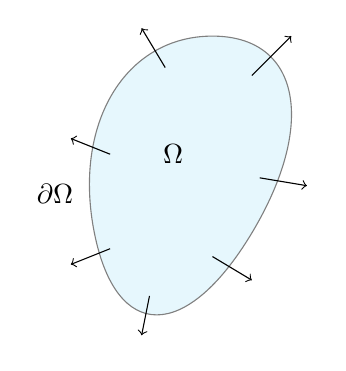
\begin{tikzpicture}
         \filldraw[fill=cyan!10!white, draw=black!50] plot [smooth cycle, tension = 2] coordinates { (0,0) (2,0) (1.5,2.5)};
         \node at (-0.5,0.5) {$\partial \Omega$};
         \node at (1,1) {$\Omega$};
        \draw[->] (2,2) -- (2.5,2.5);
        \draw[->] (0.9,2.1) -- (0.6,2.6);
        \draw[->] (0.2,1) -- (-0.3,1.2);
        \draw[->] (0.2,-0.2) -- (-0.3,-0.4);
        \draw[->] (2.1,0.7) -- (2.7, 0.6);
        \draw[->] (1.5,-0.3) -- (2, -0.6);
        \draw[->] (0.7,-0.8) -- (0.6, -1.3);
       \end{tikzpicture}
    \caption{Domain  $\Omega$.}
    \label{Fig:ConservationLaws/Domain}
    \end{center}
\end{wrapfigure}{}
%We will frequently use the following notation. 
%\begin{center}
%\begin{itemize}
%  \item[] $\mathbb{N}$ the set of natural numbers, including 0.
%  \item[]  $\mathbb{Q}$ the set of rational numbers.
%  \item[]  $\mathbb{R}$ the set of real numbers.
%  \item[]  $L_{loc}^p $ the set of locally integrable functions.
%  \item[]  $C^0 $ the set of continuous functions.
%  \item[]  $C^1 $ the set of continuous and differentiable functions.
%\end{itemize}
%\end{center}

Let $\Omega \subseteq \mathbb{R}$ and assume $\Omega$ to be an arbitrary bounded domain with piece-wise $C^1$ boundary $\partial \Omega$. We have a fluid in $\Omega$ with density $\rho = \rho(\boldsymbol{x}, t)$ and velocity $v = v(\boldsymbol x, t)$, and we can describe the the fluid inside the domain as follows:
\begin{equation*}
    \underbrace{\frac{d}{dt} \int_{\Omega} \rho dx }_{ \text{The total change of mass over time}}  = \underbrace{\int_{\partial \Omega} (\rho v) \cdot n ds }_{\text{The flow of mass over the boundary}}
\end{equation*}
Assuming $\frac{\partial \rho}{\partial t}$ is continuous in time and space, we use Leibniz rule and move the differentiation inside the integral. Furthermore, using the divergence theorem on the right hand side: 
\begin{equation*}
    \int_{\Omega} \frac{\partial \rho}{\partial t} dx   = - \int_{\Omega} \nabla \cdot (\rho v)dx 
\end{equation*}
\begin{equation*}
    \int_{\Omega} \big ( \frac{\partial \rho}{\partial t}  + \nabla \cdot (\rho v) \big ) dx   = 0.
\end{equation*}
And since the domain is arbitrary and sufficiently smooth: 
\begin{equation}
    \frac{\partial \rho}{\partial t}  + \nabla \cdot (\rho v) = 0.
\label{Burgers}
\end{equation}
One should also notice that only two simple assumptions were made, conservation of mass, and sufficient smoothness. We can generalise this formulation for a conserved quantity $u \in \mathbb{R}^n$ with flux $ f \in \mathbb{R}^m$ 
\begin{equation}
    u_t + f(u)_x = 0, 
    \label{GeneralEquation}
\end{equation}
where the flux function $f(u)$ will give rise to different models. We call equations of the form (\ref{GeneralEquation}) non-linear conservation laws, if $f(u)$ is non-linear. The one derived above, equation (\ref{Burgers}), is named the Lighthill-Whitham-Richards (LWR) model \cite{LWROrig}. We also have systems of equations, which leads to models like the Payne-Whitham Model, the Aw-Rascle Model, and multi-population models a long with multi-lane models. 

\paragraph{The Rankine-Hugoniot condition.}
When given a non-linear conservation law of the form (\ref{GeneralEquation}), our first instinct is to solve it the \textit{classical} way, by method of characteristics. However, in many cases we cannot expect to find classical solutions for all times using this method, as often the solution evolves into a multi-valued function of $x$. Figure \ref{Fig:Multivalued} shows the characteristics of a solution $u(x,t)$ to the equation (\ref{GeneralEquation}). For $t < t_0$ the characteristic lines do not intersect, and we have a classical solution. For $t \geq t_0$ the lines intersect and the classical solution can not exist. 
\begin{figure}
\begin{center}
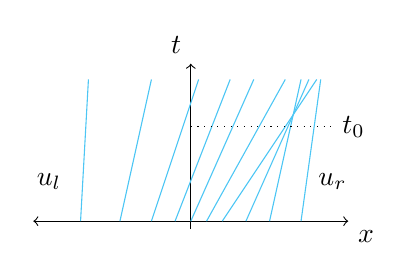
\begin{tikzpicture}
% coord.
\draw[<->] (-2,0) -- (2,0) node[anchor= north west] {$x$};
\draw[->] (0,-0.1) -- (0,2) node[anchor=south east] {$t$};
% rarefaction
\draw[color=cyan!70!white] (-1.4,0) -- (-1.3,1.8);
\draw[color=cyan!70!white] (-0.9,0) -- (-0.5,1.8);
\draw[color=cyan!70!white] (-0.5,0) -- (0.1,1.8);
\draw[color=cyan!70!white] (-0.2,0) -- (0.5,1.8);
\draw[color=cyan!70!white] (0,0) -- (0.8,1.8);
\draw[color=cyan!70!white] (0.2,0) -- (1.2,1.8);
\draw[color=cyan!70!white] (0.4,0) -- (1.6,1.8);
\draw[color=cyan!70!white] (0.7,0) -- (1.5,1.8);
\draw[color=cyan!70!white] (1,0) -- (1.4,1.8);
\draw[color=cyan!70!white] (1.4,0) -- (1.65,1.8);
\draw[dotted] (0,1.2) -- (1.8,1.2) node[anchor=west] {$t_0$};
\node at (-1.8, 0.5) {$u_l$};
\node at (1.8, 0.5) {$u_r$};
\end{tikzpicture}
\label{Fig:Multivalued}
\caption{Non-classical solution using method of characteristics.}
\end{center}
\end{figure}
Therefore, we will extend our admissable set of solutions in order to allow such discontinuities; so-called weak solutions \cite{HoldenH.Helge2015Ftfh}. 

Consider the model equation (\ref{GeneralEquation}) and define $\phi \in C_0^{\infty}(\Omega \times [0, T])$ have compact support, and assume initial condition $u|_{t=0} = u_0 $. Multiplying with the test function $\phi$, and integrating by parts over an arbitrary domain $[0,T] \times \Omega \subseteq \mathbb{R}$, we obtain
\begin{align}
    0 &= \int_0^T \int_{\Omega} (u_t + f(u)_x)\phi dxdt \nonumber \\
      &= \int_0^T \int_{\Omega_c} (\cdot) dxdt \nonumber \\ 
      &= \int_0^T \int_{\Omega} (u \phi_t + f(u)\phi_x) dxdt + \int_{\Omega} u_0 \phi(x,0) dx. 
    \label{Weak form}
\end{align}
Note that, as $\phi$ has compact support, the boundary terms vanish. Also we no longer have a requirement on $u$ and $f(u)$ to be differentiable. And lastly note that if the equation (\ref{GeneralEquation}) admits a classical solution $u$, then $u$ will also be a solution to the weak formulation, equation (\ref{Weak form}). Does this weak solution allow for the discontinuities we require?

Assume a discontinuity along a smooth curve $\Gamma : x = x(t)$, which is differentiable in a neighbourhood of $x(t)$, and that the equation (\ref{GeneralEquation}) admits a classical solution outside the discontinuity. Now we choose a neighbourhood $D = D_1 \cup D_2$ around the point $(x(t), t)$, see Figure \ref{fig:ConservationLaws/RHIsolated_disc}, and a test function with compact support in D. We investigate the weak solution on $D$:
\begin{align*}
    0 &= \iint_D( u \phi_t + f(u)\phi_x) dx dt \\
      &= (\iint_{D_1}  +  \iint_{D_2}  )( (u \phi_t + f(u)\phi_x) + \phi \underbrace{(u_t + f(u)_x )}_{=0} ) dxdt\\
      &= (\iint_{D_1}  +  \iint_{D_2}  ) ( (\phi u )_t + (\phi f(u))_x ) dxdt \\
      &= (\iint_{D_1}  +  \iint_{D_2}  ) (\partial_t, \partial_x)\cdot (\phi u, \phi f(u)) dx dt \\
      &= (\int_{\partial D_1}  +  \int_{\partial D_2}  ) (\phi u, \phi f(u)) \cdot n ds.
\end{align*}
In the last step Greens theorem was used to move from the whole domain $D$ onto the boundary. We have $\phi = 0 $ on $\partial D_1, \partial D_2$, except on $\Gamma$. Parameterising $\Gamma$ using the tangent $T = (x(t), 1)$ with normal vector $\vec{n} = (-1, x'(t))$, we get
\begin{equation*}
    0 = \int_{\Gamma} (\phi f(u), \phi u) \cdot (-1, x'(t)) dt.
\end{equation*}
\begin{wrapfigure}[16]{l}{0.4\textwidth}
    \centering
    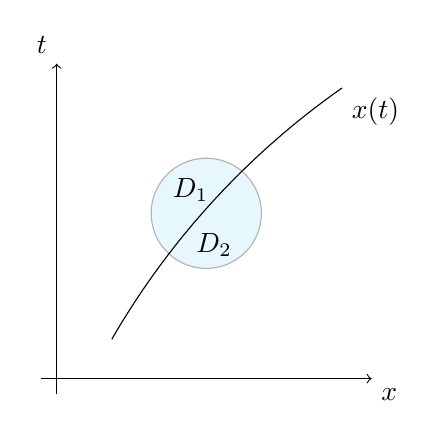
\begin{tikzpicture}
    % coordinate sys
    \draw[->] (0,-0.2) -- (0,4) node[anchor=south east] {$t$};
    \draw[->] (-0.2,0) -- (4,0) node[anchor=north west] {$x$};
    
    % plot
    \filldraw[fill=cyan!10!white, draw=black!30] (1.9, 2.1) circle (0.7cm);
    \node at (1.7,2.4) {$D_1$};
    \node at (2,1.7) {$D_2$};
    \draw (0.7,0.5) arc (150:125:10cm) node[anchor=north west] {$x(t)$};
\end{tikzpicture}
    \caption{An isolated discontinuity.}
    \label{fig:ConservationLaws/RHIsolated_disc}
\end{wrapfigure}{}
Now we want to approach the discontinuity from both sides, so we define $u_l = \lim_{\epsilon \to 0} u(x(t) - \epsilon, t)$, $u_r = \lim_{\epsilon \to 0} u(x(t) + \epsilon, t)$.
\begin{align*}
    0 &= \int_{\Gamma} (\phi x'(t) (u_r - u_l) - \phi( f(u_r) - f(u_l))  dt \\
      &= \int_{\Gamma} \phi (  f(u_r) - f(u_l) - x'(t)(u_r - u_l) ) dt.
\end{align*}
And as we have defined $\phi \geq 0 $ for all test functions, we must have
\begin{equation*}
    f(u_r) - f(u_l)  = x'(t)(u_r - u_l) 
\end{equation*}
\begin{equation}
    [f] = s[u], \quad s := x'(t) 
    \label{Eq:RH}
\end{equation}
where we have used the notation $[u] = u_r - u_r$ for the jump in a quantity $u$. This, (\ref{Eq:RH}), is called the \textit{The Rankine-Hugoniot condition}, and it describes the conservation of mass $u$ across a discontinuity. It gives a condition on discontinuities of weak solutions (\ref{Weak form}), and it relates left state $(u_l)$ and right state $(u_r)$ with the speed $x'(t)$ of the \textit{shock wave}. Also, note that this derivation of the Rankine-Hugoniot condition can easily be extended to higher dimensions, and (\ref{Eq:RH}) is a system of $n$ scalar equations \cite{GaravelloMauro2006Tfon}.

We have now seen that the weak solution permits certain discontinuities. However, we loose uniqueness with weak solutions, as the equation no longer needs to hold point-wise, and we need to find a way to restore it. We do that by introducing entropy conditions, but first we will take a look at the Riemann problem.
% ---------------------------------------------------------------------
% ---------------------------------------------------------------------
% ---------------------------------------------------------------------

\subsection{The Riemann Problem}
We will now turn our attention to the Riemann problem. The initial value problem is the Riemann problem for conservation laws (\ref{Eq: RP}). This can can be thought of as gas in a tube, separated by a membrane, see Figure \ref{Fig:riemann_tube}. On each side of the membrane we have a gas with different density.
\begin{equation}
 u_t + f(u)_x = 0,  \quad u|_{t = 0 } = \begin{cases} u_l & \text{if $x \leq 0$,}\\ u_r & \text{if $x>0$.} 
 \label{Eq: RP}
 \end{cases}
\end{equation}
\begin{wrapfigure}[10]{r}{0.5\textwidth}
    \begin{center}
        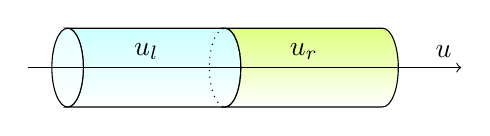
\begin{tikzpicture}
        \draw   [thin, shade,top color=cyan!20!white]  (0,-0.5) -- ++(2,0) 
    arc(-90:90:0.2 and 0.5) -- ++(-2,0) 
    arc(90:-90:0.2 and 0.5)--cycle;
        \draw   [thin, shade,top color=lime!50!white]  (2,-0.5) -- (4,-0.5) 
        arc(-90:90:0.2 and 0.5) -- ++(-2,0)
        arc(90:-90:0.2 and 0.5) --  cycle;
    \draw[thin, shade, top color=cyan!10!white] (0,0) ellipse(0.2 and 0.5);
    \draw[dotted] (2,0) ellipse(0.2 and 0.5);
        \node at (1,0.2) {$u_l$};
        \node at (3,0.2) {$u_r$};
        \draw[->] (-0.5,0) -- (5,0) node[anchor=south east] {$u$};
        \end{tikzpicture}
    \caption{Initial constant state.}
    \label{Fig:riemann_tube}
    \end{center}
\end{wrapfigure}

Note that equation is scale invariant. This means that if we scale u with some parameter, it will not change the equation or the solution. $v(x,t) = u(\alpha x, \alpha t) \rightarrow \alpha u(t,x)$. Therefore we can introduce a scaling on $u(x,t) = \omega (x/t) $, $ \xi = x/t$. We have either sharp discontinuities \textit{shocks} from $u_l$ to $u_r$ or solutions that smooth out \textit{rarefactions} from point $u_l$ to $u_r$. 
 \begin{equation*}
     \begin{split}
         0 &= u_t + f(u)_x = u_t + df(u)u_x \\
           &= \dot \omega( -\frac{x}{t^2}) + df( \omega) \dot \omega t^{-1} \\
           &= \frac{x}{t}(  df( \omega) \dot \omega - x/t \dot \omega ).
     \end{split}
 \end{equation*}
 And we have the resulting equation 
 \begin{equation}
     df( \omega) \dot \omega =  \xi \dot \omega.
     \label{Eq:scaledEq}
 \end{equation}

\subsubsection{The scalar conservation law}
Let $u,f \in \mathbb{R}$. We can then cancel $\dot \omega $ in (\ref{Eq:scaledEq}), and if $f'$ is strictly monotone, we can find $u(x,t) = w(x/t) = (f')^{-1}(\frac{x}{t})$. 
To ensure strict monotonicity, we introduce the lower convex envelope $f_{\smile}(u) = \sup\{g(u) : g\leq f, \quad  g \quad \textit{convex on}\quad [u_l, u_r]\} $. We claim we have the solution for $u_r > u_l$:
 \begin{equation}
     u(x,t) = \begin{cases} u_l & \text{for $x < f'_{\smile} (u_l)t$,}\\
                            (f'_{\smile} )^{-1}(\frac{x}{t}) & \text{for $f'_{\smile} (u_l)t$} < x < f'_{\smile} (u_r)t,\\ 
                            u_r & \text{for $x > f'_{\smile} (u_r)t$}. 
     \end{cases}
     \label{Eq:ScalarRiemannSol}
 \end{equation}
We can also construct the upper concave envelope, in case $u_r < u_l$, by transforming $x \mapsto -x$. We now have $-f(u)$, and the lower convex envelope of $-f$, which is the upper concave envelope from $u_l$ to $u_r$.  Where $f_{\frown}(u) = \inf\{g(u) : g\leq f, \quad g \quad \textit{concave on} \quad  [u_r, u_l]\} $. And the principle is the same, replacing with $f_{\frown}(u)$ in (\ref{Eq:ScalarRiemannSol}). 

  \begin{minipage}{\linewidth}
  \centering
  \begin{minipage}{0.45\linewidth}
      \begin{figure}[H]
          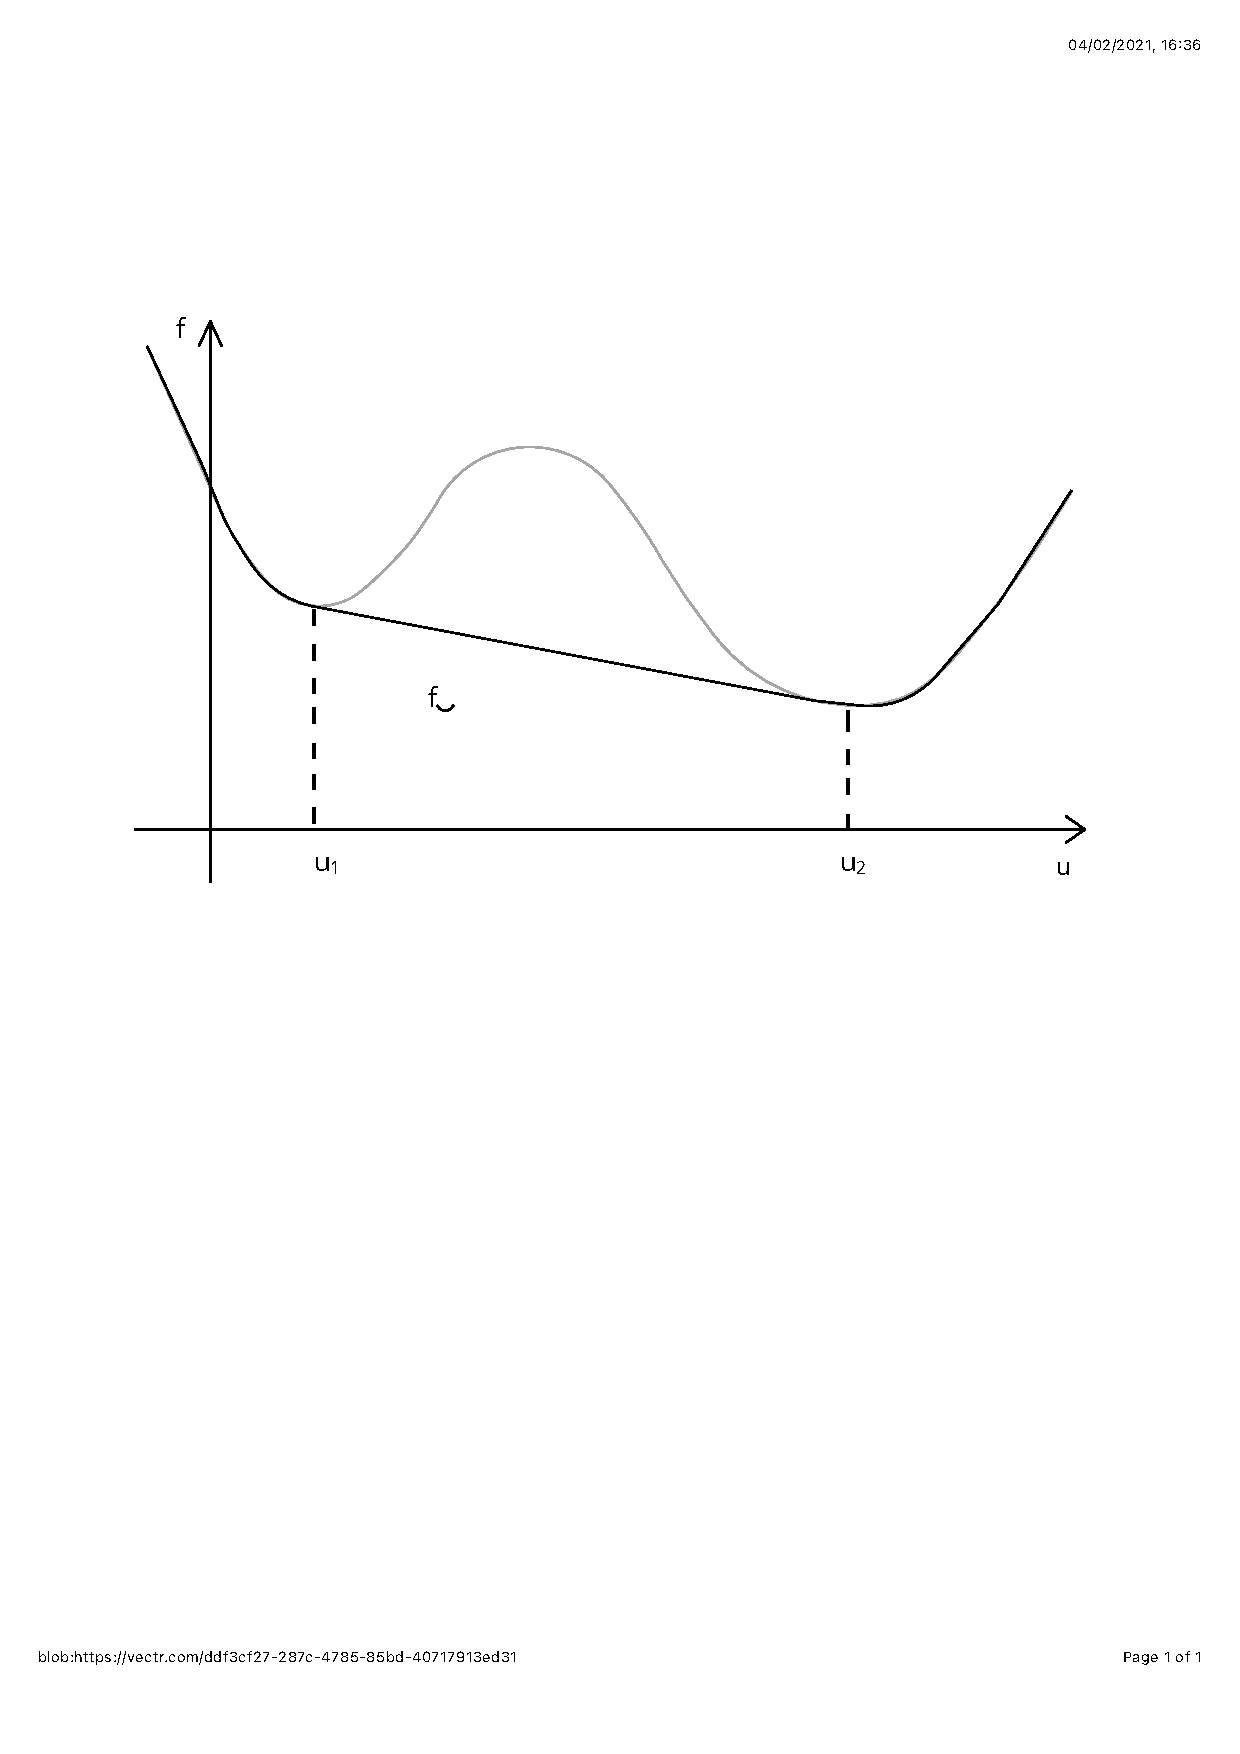
\includegraphics[clip, trim=2cm 14cm 2cm 2cm, width=0.99\textwidth]{Figures/ConservationLaws/convex_envelope.pdf}
          \caption{The convex envelope of $f$.}
          \label{Fig:covexenvelope}
      \end{figure}
  \end{minipage}
  \hspace{0.05\linewidth}
  \begin{minipage}{0.45\linewidth}
      \begin{figure}[H]
          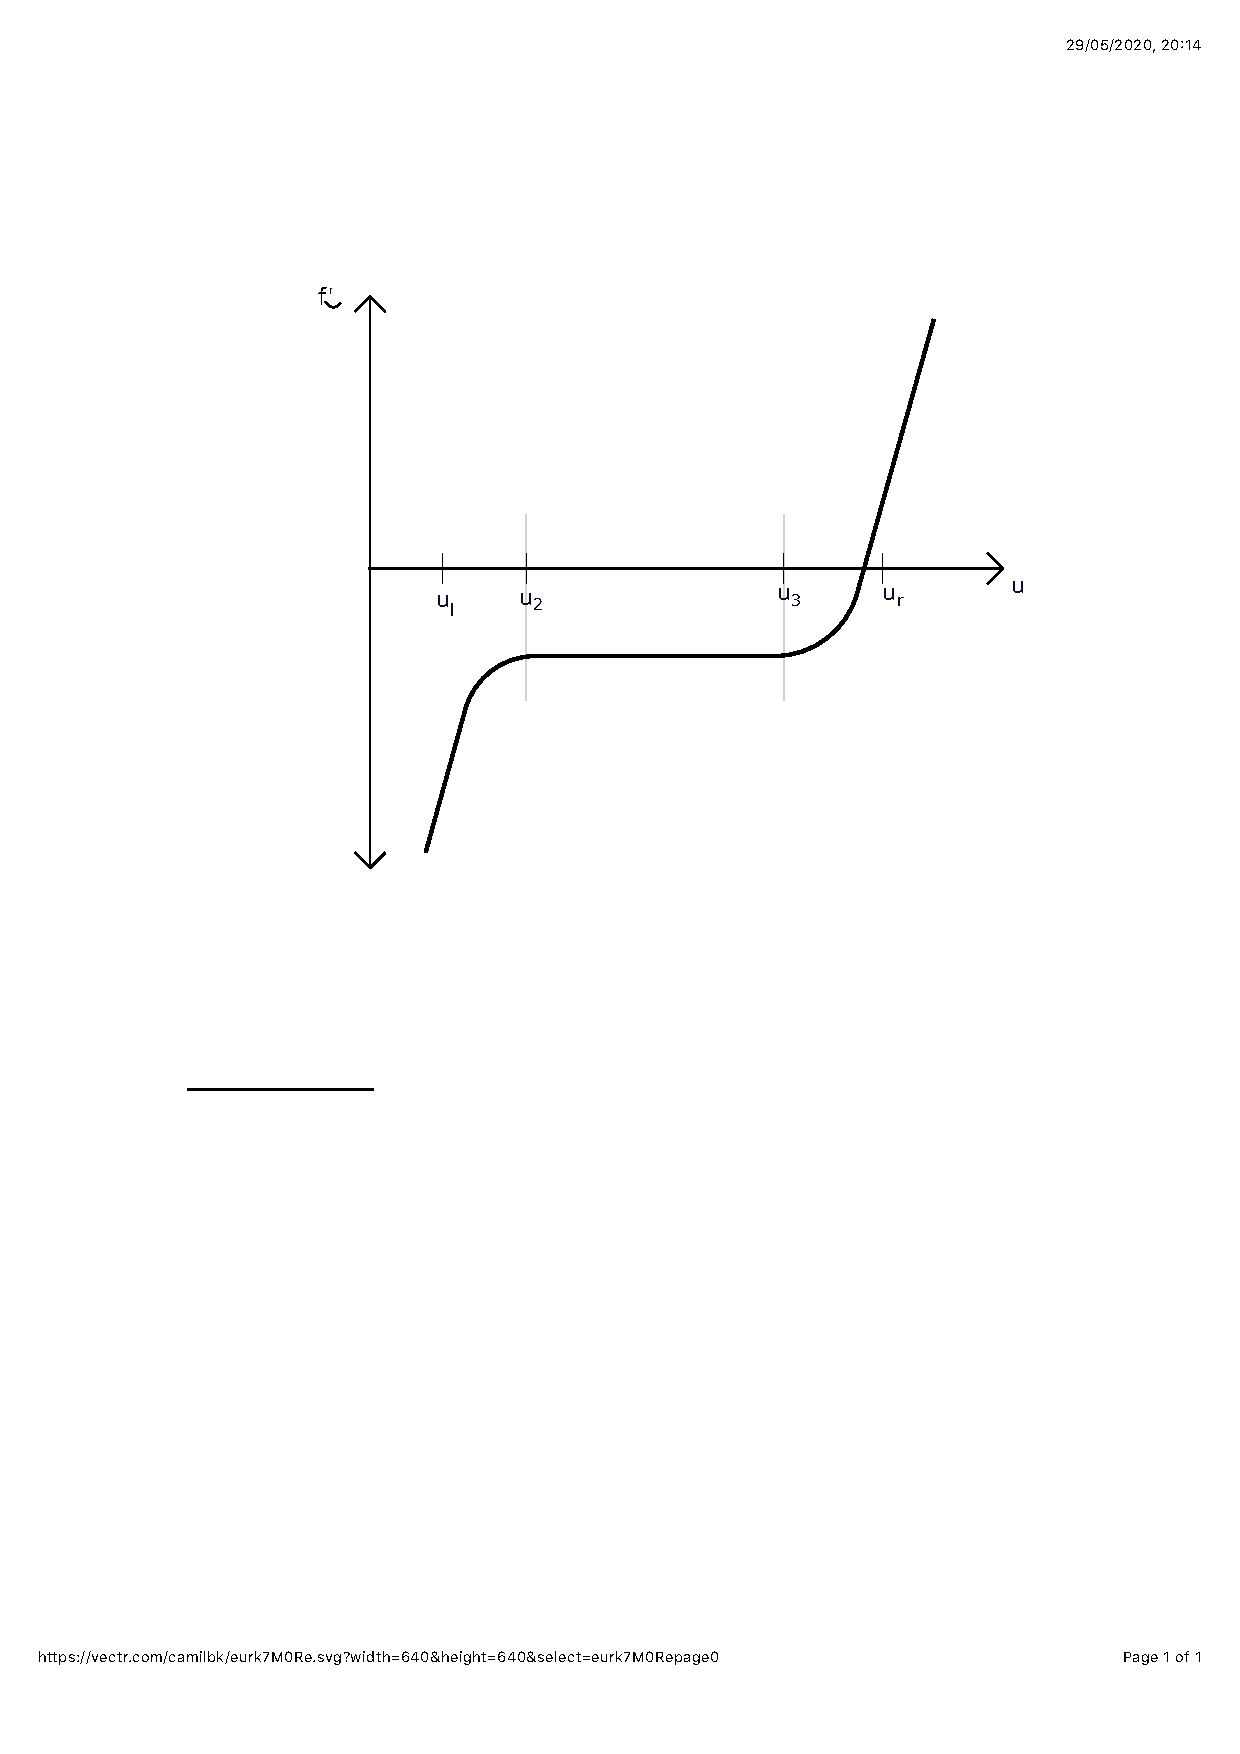
\includegraphics[clip, trim=2cm 14cm 2cm 2cm, width=0.99\textwidth]{Figures/ConservationLaws/convex_derivative.pdf}
          \caption{The derivative of the convex envelope of $f$.}
          \label{Fig:derivativeOfEnvelope}
      \end{figure}
  \end{minipage}
\end{minipage}  

 It turns out that this simple idea is the key to solving the Riemann problem for scalar conservation laws. Now $f''_{\smile, \frown} \geq 0$ and $f'_{\smile, \frown} $ is non-decreasing. This allows us to take the inverse regardless of the shape of $f$, and permitting Rankine-Hugoniot discontinuities where $f'_{\smile, \frown} $ is constant. A discontinuity that satisfies the Rankine-Hugoniot entropy condition is called a \textit{shock wave}, and the continuous parts of (\ref{Eq:ScalarRiemannSol}) are called \textit{rarefaction waves} \cite{HoldenH.Helge2015Ftfh}. Now (\ref{Eq:ScalarRiemannSol}) makes sense for both rarefactions and shocks. If $f \in C^2$ has finitely many inflection points, there will be finitely many intervals alternating $f_{\smile, \frown} $ and $f(u)$. We construct the solution $u(\cdot, t)$ of finitely many intervals using these fluxes. This $u$, it turns out, is a weak solution as it satisfies (\ref{GeneralEquation}) and the so called \textit{travelling wave condition}. Notice we have the same derivative at $u_2$ and $u_3$, see Figure \ref{Fig:covexenvelope}, \ref{Fig:derivativeOfEnvelope} so Rankine-Hugoniot is satisfied as well. We state the result below
\begin{theorem}
The initial value problem
\begin{equation*}
    u_t + f(u)_x = 0,  \quad u|_{t = 0 } = \begin{cases} u_l & \text{for $x \leq 0$,}\\ u_r & \text{for $x>0$.} 
 \end{cases}
\end{equation*}
 with a flux function $f(u)$ such that $f_{\smile,\frown} \neq f$ on finitely many intervals, alternating with intervals where they coincide, has a weak solution given by the equation (\ref{Eq:ScalarRiemannSol}) if $u_l > u_r$. And if $u_r > u_l$, we construct a concave envelope.  
\label{RP_Kruzkov_sol}
\end{theorem} For the proof, along with the Kružkov theory, see Chapter $2$ in \cite{HoldenH.Helge2015Ftfh}.


% ---------------------------------------------
% ---------------------------------------------

\subsubsection{The conservation law for systems }
Let $u, f \in \mathbb{R}^n$ and  $ df(u)$ be the non-linear Jacobian matrix of the system. However, in this case we cannot cancel $ \dot \omega$ in (\ref{Eq:scaledEq}) as in the scalar case, and we are left with an eigenvalue problem. We will assume that the Jacobian $df(u)$ has $n$ real eigenvalues 
\begin{equation}
    df(u)r_j(u) = \lambda_j(u)r_j(u), \quad \lambda_j(u) \in \mathbb{R}, \quad j = 1, \dots, n. 
    \label{Eq:Eig.val problem}
\end{equation}
If the eigenvalues $\lambda_1 \leq \lambda_2 \leq \dots \leq \lambda_n $ are real, we have a hyperbolic system. If the eigenvalues are distinct, the system is strictly hyperbolic \cite{HoldenH.Helge2015Ftfh}. 

\paragraph{Rarefaction waves.}
From the assumptions of the Riemann problem (\ref{Eq: RP}), and the assumptions on the flux function (\ref{Eq:Eig.val problem}) we have the following \begin{equation*}
     df( \omega) \dot \omega =  \xi \dot \omega,
\end{equation*} \begin{equation}
    \begin{cases}
    \omega( \lambda_j( u_l) ) = u_l, \\
    \omega( \lambda_j( u_r) ) = u_r, \\
    \end{cases}
    \quad \quad
    \begin{cases}
    \dot \omega( \xi ) = r_j( \omega(\xi)), \\
    \lambda_j (\omega(\xi)) = \xi. \\
    \end{cases}
    \label{Eq:SystemsAssumptions}
\end{equation}
From (\ref{Eq:SystemsAssumptions}), for a fixed time $t$ the function $\omega(x/t)$ will connect $u_l$ to $u_r$. For the case $u_l < u_r$, $\xi$ must be increasing, hence $\lambda_j( \omega(x/t)$ must be increasing. We call these solution curves, emanating from $u_l$, \textit{rarefaction waves} $u_r \in R_j(u_l)$
\begin{equation}
     u(x,t) = \begin{cases} u_l & \text{for $x < \lambda_j(u_l)t$,}\\
                            \omega(\frac{x}{t}) & \text{for $ \lambda_j(u_l)t$} < x <  \lambda_j(u_r)t,\\ 
                            u_r & \text{for $x >  \lambda_j(u_r)t$.} 
     \end{cases}
     \label{Eq:SystemRarefactionSol}
 \end{equation}
where $\omega(\xi)$ satisfies the assumptions (\ref{Eq:SystemsAssumptions}). Looking at $\dot \omega( \xi ) = r_j( \omega(\xi))$ along with the initial condition $\omega( \lambda_j( u_l) ) = u_l$ the integral curves in the $u$ plane is denoted $R_j(u_l)$.  Similarly, we can do this for $u_r$ and obtain the rarefaction curve emanating from $u_r$. For complete roof, and mathematical justification see Chapter $5$ in \cite{HoldenH.Helge2015Ftfh}. 

We investigate further the last assumption from (\ref{Eq:SystemsAssumptions}), $ \lambda_j (\omega(\xi)) = \xi$, and taking the derivative with respect to $\xi$ we obtain
\begin{align*}
    \frac{d}{d\xi} \xi &= \frac{d}{d\xi} \lambda_j( \omega (\xi)) \\
    1 &= \nabla \lambda_j (\omega(\xi)) \cdot \dot \omega (\xi) = \nabla \lambda_j \cdot r_j(\xi),
    \label{Eq:DirectionOfLambda}
\end{align*} 
which imposes an extra condition on the eigenvector fields. However, if we have constant velocities $\xi, \lambda_j$ this will not hold, as we are unable to normalise the eigenvector. We say the $j$th family 
\begin{align*}
    \nabla \lambda_j \cdot r_j = 1 \quad \text{is genuinely nonlinear, } \\
    \nabla \lambda_j \cdot r_j = 0 \quad \text{is linearly degenerate. }
\end{align*}

Lastly we introduce Riemann invariants, which are useful when solving the Riemann problem for systems. \begin{definition}[Riemann invariants]
A smooth function $\omega : \mathbb{R}^n \mapsto \mathbb{R}$ is called a \textit{k-Riemann invariant} if 
\begin{align*}
    \nabla \omega(u) \cdot r_k (u) = 0,
\end{align*}
where $r_k$ is the k'th right eigenvector of the strictly hyperbolic Jacobian.
\end{definition}
From the definition of Riemann invariants one can show that the rarefaction curves are constant on all Riemann invariants, and thus we can use this as an alternative definition of rarefaction curves. This will be useful when investigating our model for traffic in Section $3$.  

\paragraph{Contact Discontinuities.}
\begin{comment}
From (\ref{Eq:DirectionOfLambda}) recall $\lambda_j(u)$ is increasing along the rarefaction curve $R_j(u_l)$, we can take advantage of this direction and define a parameter $\epsilon := \xi - \xi_l = \lambda_j(u)-\lambda_j(u_l) > 0$. We denote the corresponding $u$ by $u_{j,\epsilon} = \omega(\lambda_j(u)) = \omega(\epsilon + \lambda_j(u_l))$. 
\end{comment}
Investigating the linearly degenerate case, we want to create a phase path of the eigenvector field. In this case, $\lambda$ is constant along the integral curve, and we have 
\begin{align*}
    \frac{d}{d\xi} f(u) = df(u) \dot u = df(u) \cdot r_j = \lambda_j \cdot r_j = \lambda_j \dot u \\
     \frac{d}{d\xi} \lambda = \nabla \lambda_j \cdot r_j = 0 \\
     \frac{d}{d\xi} f(u) =  \frac{d}{d\xi}( \lambda_j u ) \\
     f(u) = \lambda_j u. 
\end{align*}

The Rankine-Hugoniot relation is retrieved. We call this solution curve in the phase plane a contact discontinuity $C_j(u_l)$, passing through $u_l$. For each $u_r \in C_j(u_l)$ the initial value problem (\ref{Eq: RP}) has a solution \begin{equation}
    u(x,t) = \begin{cases}
    u_l \quad \text{for} \quad x < \lambda_j(u_l)t, \\
    u_r \quad \text{for} \quad x \geq \lambda_j(u_l)t. 
    \end{cases}
    \label{Eq:ContactDiscSol}
\end{equation} 
The rarefaction and the shock curves must necessarily be the same in this case. Also, the weak solution is satisfied. Again, for complete roof, and mathematical justification see Chapter $5$ in \cite{HoldenH.Helge2015Ftfh}. 

\paragraph{Shock waves. }
The obvious extension is to define the shock curves in the phase plane. Now assume $u_l$ is fixed, and we consider all possible states $u$ that satisfy the Rankine-Hugoniot relation. We call the trajectories in the phase plane the \textit{Hugoniot Locus}:
\begin{equation}
    \label{Hugoniot_locus}
    H(u_l) := \{ u : \exists s\in \mathbb{R} \quad \text{such that} \quad s[u] = [f] \}.
\end{equation}
However, the system $ \mathcal{H} := s[u] - [f] = 0 $ has $n$ equations, so we have $n+1$ unknowns in our case. Using the implicit function theorem we can prove that in a neighbourhood of $u_l$ we have $n$ unique differentiable solutions, only requiring that $d \mathcal{H}$ is non-singular (see Chapter $5$, theorem $5.11$ in \cite{HoldenH.Helge2015Ftfh}). 
 
\paragraph{The Lax entropy.} We have now found three types of solution curves which may arise when studying a strictly hyperbolic system of the form (\ref{GeneralEquation}). Emanating for a point $u_l$ we have at most $2n$ waves, $n$ rarefaction- and $n$ shock curves. We need to find a way to eliminate half of these possibilities to restore uniqueness. We do this by introducing Lax entropy. 
%In the systems case, $\dot U = f(U) - f(u_l) - s(U-u_l)$ will give the flow in the eigenvectorspace, and determines whether or not we can connect $u_l$ to $u_r$. 

In the case of systems, the eigenvalues in the critical point determines the behaviour of the eigenvector field. In our (real) case, we have the following possibilities, $\boldsymbol{\lambda} > 0 $ source, $\boldsymbol{\lambda} < 0 $ sink, $\lambda_i < 0 < \lambda_j $ saddle \cite{VerhulstFerdinand1990NDEa}.
It is clear that for there to exist an orbit from $u_l$ to $u_r$, $u_l$ cannot be a pure sink, and $u_r$ cannot be a pure source. This means we go from $9$ different combinations, down to $4$, and can be seen in the Figure \ref{fig:LaxMotivation}. 
\begin{figure}[H]
    \centering
    \begin{minipage}{.2\textwidth}
    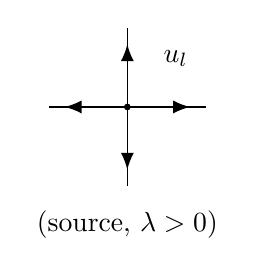
\begin{tikzpicture}
    [decoration={markings, 
            mark= at position 0.8 with {\arrow[line width=0.4mm]{latex}} }
    ] 
    \draw[postaction = {decorate}] (1,0) -- (0,0); 
    \draw[postaction = {decorate}] (1,0) -- (2,0); 
    \draw[postaction = {decorate}] (1,0) -- (1,1);
    \draw[postaction = {decorate}] (1,0) -- (1,-1);
    \filldraw[black] (1,0) circle (1pt) ;
    \node at (2, 1,1) {$u_l$};
    \node at (1,-1.5) {(source, $\lambda > 0$)};
    \end{tikzpicture}
    \end{minipage}
    \begin{minipage}{.2\textwidth}
    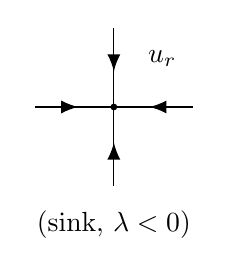
\begin{tikzpicture}
    [decoration={markings, 
            mark= at position 0.55 with {\arrow[line width=0.4mm]{latex}} }
    ] 
    \draw[postaction = {decorate}] (0,0) -- (1,0); 
    \draw[postaction = {decorate}] (2,0) -- (1,0); 
    \draw[postaction = {decorate}] (1,1) -- (1,0);
    \draw[postaction = {decorate}] (1,-1) -- (1,0);
    \filldraw[black] (1,0) circle (1pt) ;
    \node at (2, 1,1) {$u_r$};
    \node at (1,-1.5) {(sink, $\lambda < 0$)};
    \end{tikzpicture}
    \end{minipage}
    \quad
    \begin{minipage}{.2\textwidth}
    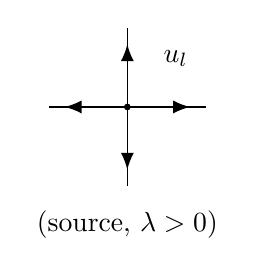
\begin{tikzpicture}
    [decoration={markings, 
            mark= at position 0.8 with {\arrow[line width=0.4mm]{latex}} }
    ] 
    \draw[postaction = {decorate}] (1,0) -- (0,0); 
    \draw[postaction = {decorate}] (1,0) -- (2,0); 
    \draw[postaction = {decorate}] (1,0) -- (1,1);
    \draw[postaction = {decorate}] (1,0) -- (1,-1);
    \filldraw[black] (1,0) circle (1pt) ;
    \node at (2, 1,1) {$u_l$};
    \node at (1,-1.5) {(source, $\lambda > 0$)};
    \end{tikzpicture}
    \end{minipage}
    \begin{minipage}{.2\textwidth}
    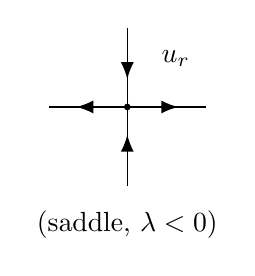
\begin{tikzpicture}
    [decoration={markings, 
            mark= at position 0.65 with {\arrow[line width=0.4mm]{latex}} }
    ] 
    
    \draw[postaction = {decorate}] (1,0) -- (0,0); 
    \draw[postaction = {decorate}] (1,0) -- (2,0); 
    \draw[postaction = {decorate}] (1,1) -- (1,0);
    \draw[postaction = {decorate}] (1,-1) -- (1,0);
    \filldraw[black] (1,0) circle (1pt) ;
    \node at (2, 1,1) {$u_r$};
    \node at (1,-1.5) {(saddle, $\lambda < 0$)};
    \end{tikzpicture}
    \end{minipage}
    
    \begin{minipage}{.2\textwidth}
    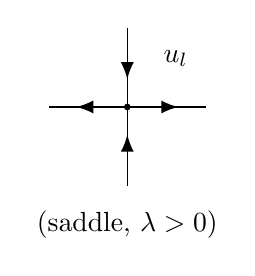
\begin{tikzpicture}
    [decoration={markings, 
            mark= at position 0.65 with {\arrow[line width=0.4mm]{latex}} }
    ] 
    \draw[postaction = {decorate}] (1,0) -- (0,0); 
    \draw[postaction = {decorate}] (1,0) -- (2,0); 
    \draw[postaction = {decorate}] (1,1) -- (1,0);
    \draw[postaction = {decorate}] (1,-1) -- (1,0);
    \filldraw[black] (1,0) circle (1pt) ;
    \node at (2, 1,1) {$u_l$};
    \node at (1,-1.5) {(saddle, $\lambda > 0$)};
    \end{tikzpicture}
    \end{minipage}
    \begin{minipage}{.2\textwidth}
    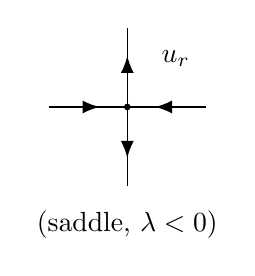
\begin{tikzpicture}
    [decoration={markings, 
            mark= at position 0.65 with {\arrow[line width=0.4mm]{latex}} }
    ] 
    \draw[postaction = {decorate}] (0,0) -- (1,0); 
    \draw[postaction = {decorate}] (2,0) -- (1,0); 
    \draw[postaction = {decorate}] (1,0) -- (1,1);
    \draw[postaction = {decorate}] (1,0) -- (1,-1);
    \filldraw[black] (1,0) circle (1pt) ;
    \node at (2, 1,1) {$u_r$};
    \node at (1,-1.5) {(saddle, $\lambda < 0$)};
    \end{tikzpicture}
    \end{minipage}
    \quad
    \begin{minipage}{.2\textwidth}
    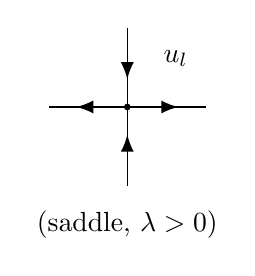
\begin{tikzpicture}
    [decoration={markings, 
            mark= at position 0.65 with {\arrow[line width=0.4mm]{latex}} }
    ] 
    \draw[postaction = {decorate}] (1,0) -- (0,0); 
    \draw[postaction = {decorate}] (1,0) -- (2,0); 
    \draw[postaction = {decorate}] (1,1) -- (1,0);
    \draw[postaction = {decorate}] (1,-1) -- (1,0);
    \filldraw[black] (1,0) circle (1pt) ;
    \node at (2, 1,1) {$u_l$};
    \node at (1,-1.5) {(saddle, $\lambda > 0$)};
    \end{tikzpicture}
    \end{minipage}
    \begin{minipage}{.2\textwidth}
    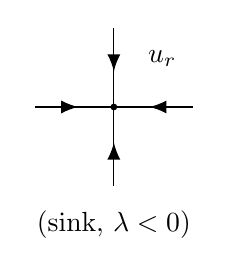
\begin{tikzpicture}
    [decoration={markings, 
            mark= at position 0.55 with {\arrow[line width=0.4mm]{latex}} }
    ] 
    \draw[postaction = {decorate}] (0,0) -- (1,0); 
    \draw[postaction = {decorate}] (2,0) -- (1,0); 
    \draw[postaction = {decorate}] (1,1) -- (1,0);
    \draw[postaction = {decorate}] (1,-1) -- (1,0);
    \filldraw[black] (1,0) circle (1pt) ;
    \node at (2, 1,1) {$u_r$};
    \node at (1,-1.5) {(sink, $\lambda < 0$)};
    \end{tikzpicture}
    \end{minipage}
    \caption{Admissible solutions of critical points.}
    \label{fig:LaxMotivation}
\end{figure}

In $n$ dimensions, we can have a combination of positive of negative eigenvalues.  When examining the possible flows in the eigenvector field, it is clear that at least one eigenvalue at $u_l$ needs to be larger than the one in $u_r$. for there to be an orbit connecting them. We summarise this argument into Lax' entropy condition
\begin{equation}
    \lambda_{j}(u_r) < s < \lambda_{j}(u_l), \quad \text{for orbits from $u_l$ to $u_r$}.
\end{equation}

\begin{definition}[Lax j-shock]
We say that a shock is a Lax j-shock if the speed satisfies the Rankine Hugoniot relation and 
\begin{align*}
    \lambda_{j-1}(u_l) < s < \lambda_{j}(u_l), \\
    \lambda_{j}(u_r) < s < \lambda_{j+1}(u_r).
\end{align*}
\end{definition}
For complete mathematical justification and proof see Chapter $5$ and Theorem $5.14$ in \cite{HoldenH.Helge2015Ftfh}. 
\begin{comment}
\subsubsection{The Kruzkov entropy}\label{The Kruzkov entropy}
Let $\eta = \eta(u)$ be a smooth convex function, and $\phi > 0$ our usual test function, $\phi \in C_0^\infty(\mathbb{R} \times (0, \infty))$ with compact support away from the x-axis. We will now investigate the case

\begin{align}
   0 &= \int_0^T \int_{\mathbb{R}} (u_t + f(u)_x - \epsilon u_{xx}) \eta' \phi dxdt \\
   &= \int_0^T \int_{\mathbb{R}} \underbrace{\eta'u_t}_{\eta_t}  \phi dx dt + \int_0^T \int_{\mathbb{R}} \underbrace{f'(u)\eta'}_{q'} u_x \phi dxdt - \epsilon \int_0^T \int_{\mathbb{R}} \underbrace{ u_{xx}\eta'}_{(\eta'u_x)_x - \eta''u_x^2}\phi dxdt \\
   &= \int_0^T \int_{\mathbb{R}}  \eta \phi_t dx dt + \int_0^T \int_{\mathbb{R}} q \phi_x dxdt  - \epsilon \int_0^T \int_{\mathbb{R}} \underbrace{ \eta'' (u_x)^2 \phi}_{ \geq 0} dxdt +  \epsilon \int_0^T \int_{\mathbb{R}} \eta \phi_{xx} dxdt \\
   & \leq \int_0^T \int_{\mathbb{R}} \bigg ( \eta \phi_t + q\phi_x + \epsilon \eta \phi_{xx} \bigg ) dx dt 
\end{align}    

\todo{fill in some details from the proof above}
Letting $\epsilon$ go to zero

\begin{equation}
    \int_0^T \int_{\mathbb{R}}( \eta \phi_t + q \phi_x)dxdt \geq 0
    \label{Kruzkov_distributions}
\end{equation}

We get the Kružkov entropy condition, in the sense of distributions. 

\begin{wrapfigure}[13]{L}{0.5\textwidth}
    \begin{center}
        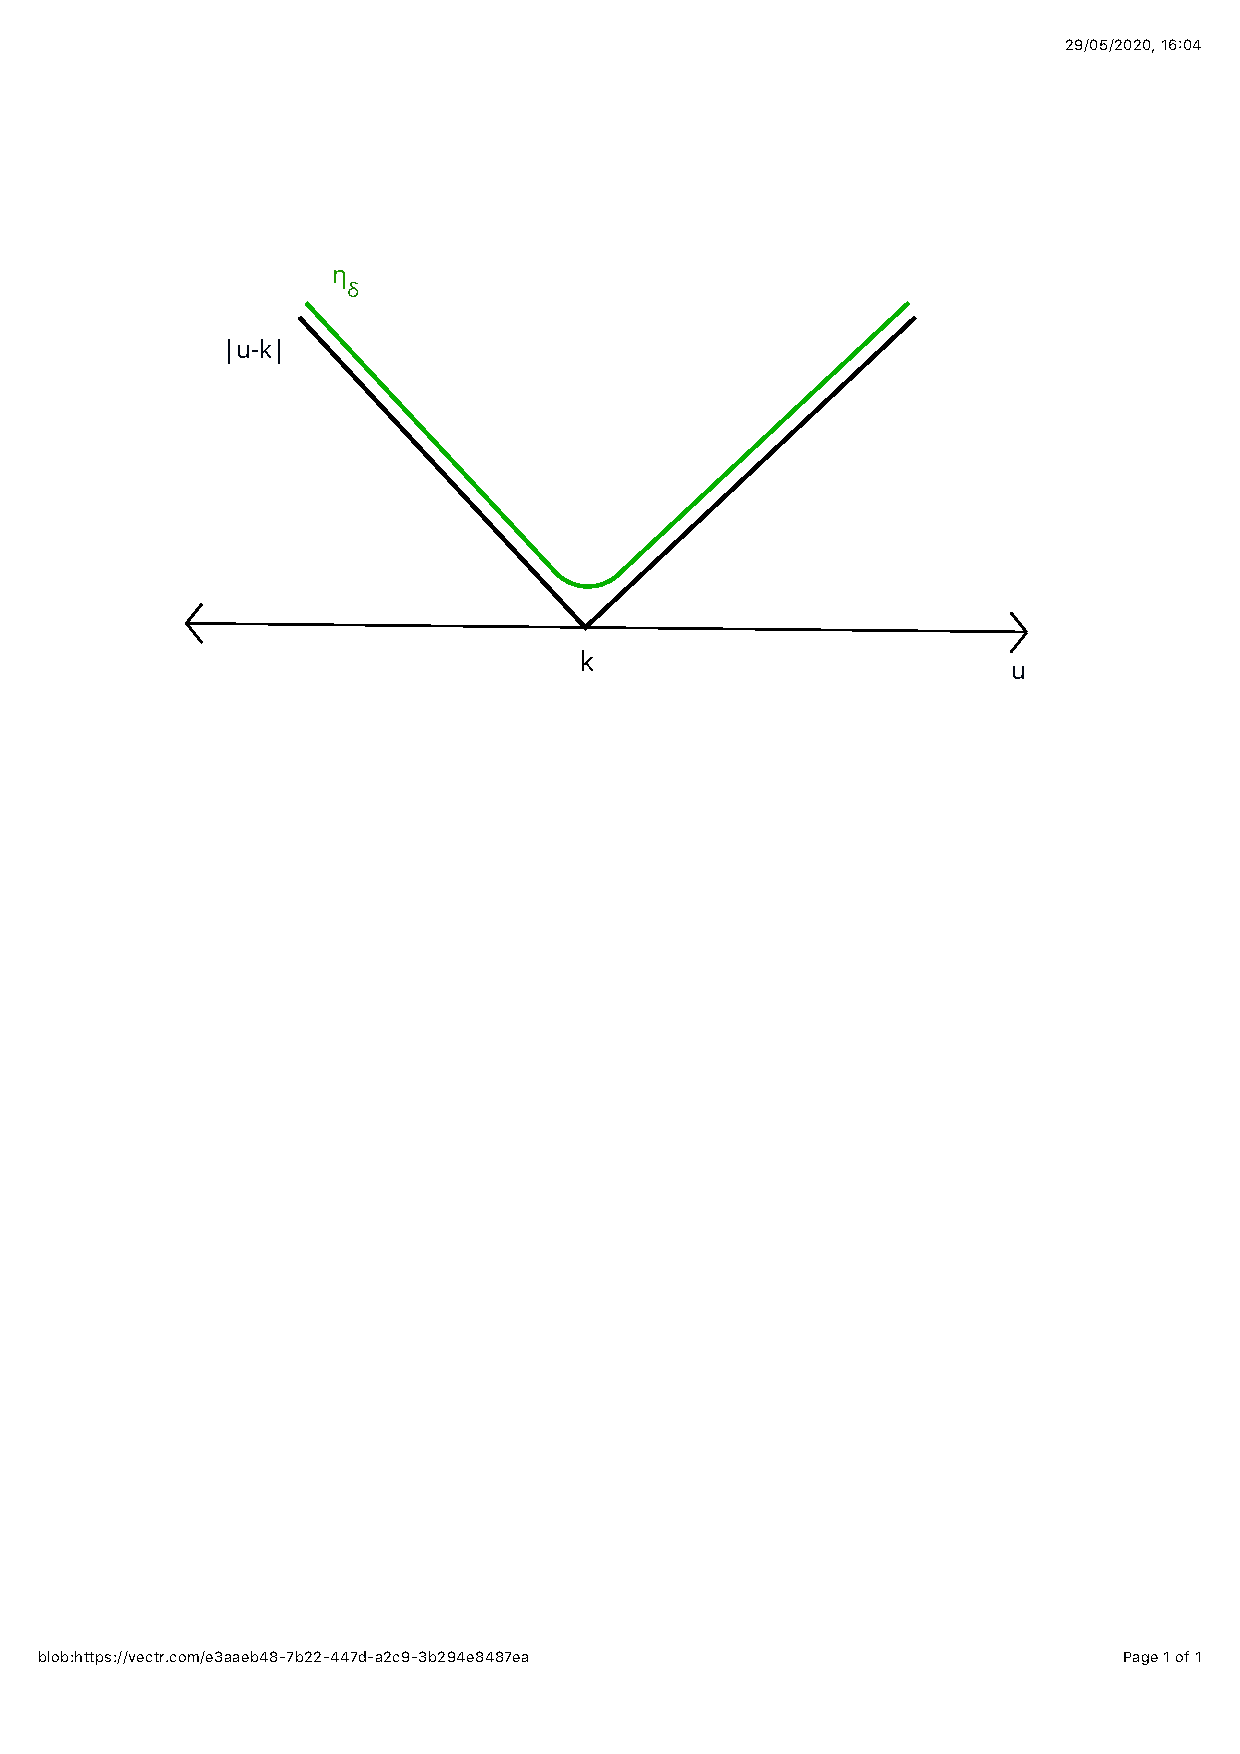
\includegraphics[valign = c,clip, trim=2cm 18cm 2cm 2cm, width=0.4\textwidth]{Figures/ConservationLaws/convex.pdf}
    \caption{Convex function}
    \label{Fig:convex}
    \end{center}
\end{wrapfigure}{}
	  
Now, let us examine a generic convex function $\eta_\delta = \sqrt{(u-k)^2 + \delta^2}$, $\delta > 0 $.  Note that  $\lim_{\delta \to 0} = |u-k|$. And recall from above that we used $q' = \eta' f'(u)$, integrating we have

\begin{equation}
    q(u) = \int_k^u \eta' f'(v) dv = sgn(u-k)(f(u) - f(k))
\end{equation}

And we get the \textit{Kružkov entropy} condition

\begin{equation}
    \iint ( |u-k|\phi_t + sgn(u-k)( f(u) - f(k))\phi_x) dx dt \geq 0
    \label{Kruzkov}
\end{equation}

If $u$ satisfies this, its called a Kružkov entropy solution for all $k$ in $\mathbb{R}$.  If we let k be less than either $u_l$ or $u_r$ we retrieve Rankine-Hugoniot. And let $k$ be greater than $u_l$ or $u_r$ we also retrieve Rankine Hugoniot. Which implies that Kružkov is a weak solution. Also, note that we can easily extend this to include the initial condition. This would have given us an extra term $- \int_\mathbb{R} \eta \phi |_{t= 0}^{t = T} dx$

 We can approximate eta as a sum of piecewice convex linear functions. Such that any convex piecewise lin. function converges to eta in $L^{inf}$. This means that Kružkov holds for all convex functions. \todo{Add proof of convex functions}

We can show that Theorem \ref{RP_Kruzkov_sol} satisfies the Kruzkov entropy condition \ref{Kruzkov}. 
To complete the proof of \ref{RP_Kruzkov_sol}, we need to show that \ref{ScalarRiemannSol} indeed satistfies the Kruzkov entropy. 

The solution u consists of a finite number of discontinuities (shocks), seperated by wedges, and the continous parts are rarefaction waves. The solution of the Riemann problem consists of a finite sequence of rarefaction waves alternating with shocks.

\begin{equation}
    \begin{split}
        \int_0^T \int_{\mathbb{R}} \big ( \eta \phi_t + q\phi_x\big ) dx dt &=  \sum_i \int \int_{\Omega_i}(\eta_i\phi_t + q_i\phi_x)dxdt \\
        &=  \sum_i \int \int_{\Omega_i}(\eta_i\phi_t + q_i\phi_x + \underbrace{(\eta_t + q_x)}_{=0}\phi )dxdt \\ &= \sum_i\int \int_{\Omega_i}( (\eta_i \phi)_t + (q_i \phi)_x )dxdt 
    \end{split}
\end{equation}

\begin{wrapfigure}[14]{R}{0.5\textwidth}
    \begin{center}
        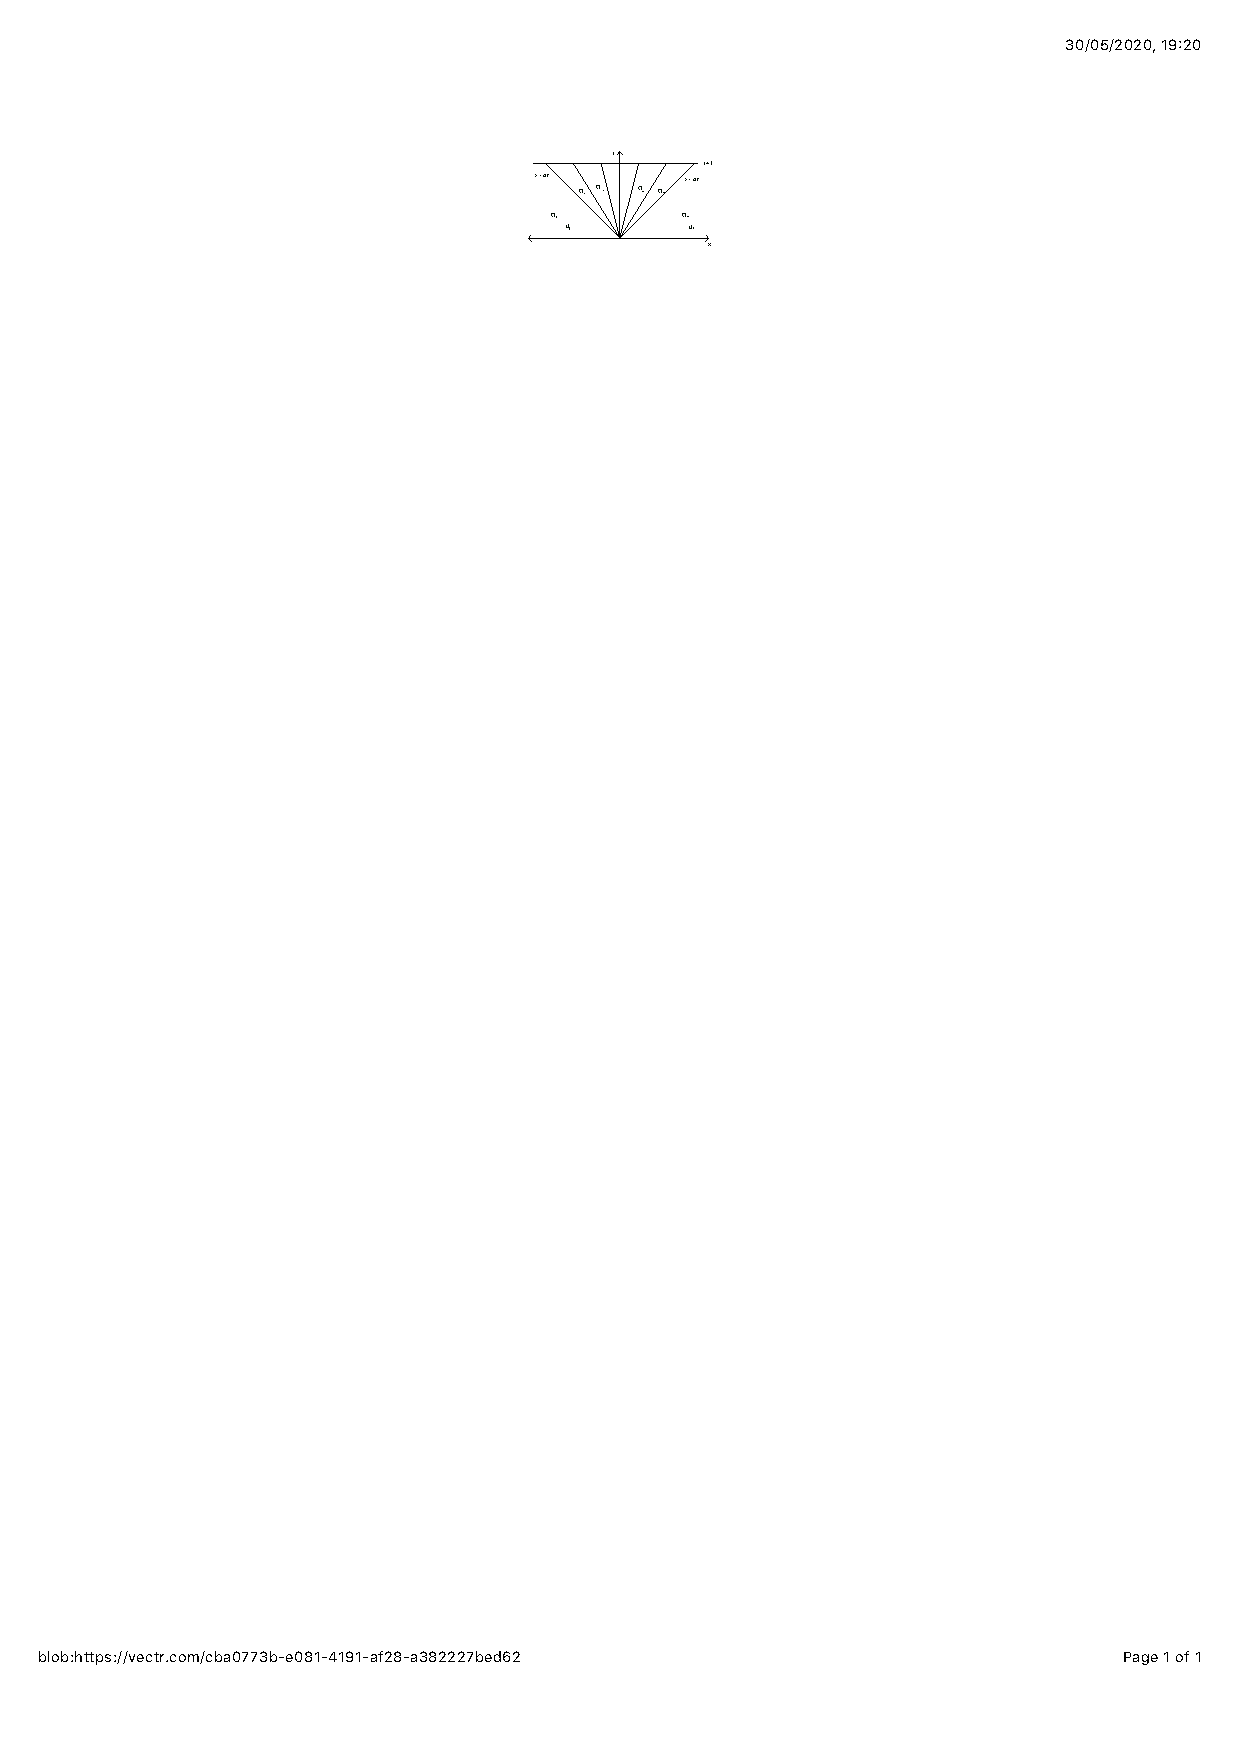
\includegraphics[valign = c,clip, trim=8cm 25.5cm 2cm 2.5cm, width=1.2\textwidth]{Figures/ConservationLaws/discrete_domain.pdf}
    \caption{Discrete domain}
    \label{Fig:discrete_domain}
    \end{center}
\end{wrapfigure}{}	 

Note that Theorem 2.2 does not require the flux function f to be differentiable. Assume now that the flux function is a polygon, i.e., that $f$ is continuous and piece- wise linear on a finite number of intervals. Thus $f'$ will then be a step function taking a finite number of values.    This means that the envelopes also will be stepfunctions. If the initial states in a Riemann problem are breakpoints, then the entire solution will take values in the set of breakpoints.



\begin{equation}
\begin{split}
    \int_0^T \int_{\mathbb{R}} \big ( \eta \phi_t + q\phi_x\big ) dx dt &= \sum_i \int\int_{\partial \Omega_i}( -(\eta_i \phi)dt + (q_i \phi)dx )) \\
    &= \sum_i \int_{\partial \Omega_i} \phi(q_i,\eta_i) \cdot \Vec{n} ds \\
    &= \int_{\mathbb{R}} \eta \phi \bigg|_{t=0}^{t=T} dx + \sum_i \int_0^T \underbrace{\phi(\sigma_it,t)}_{\geq 0} \underbrace{\bigg( \sigma_i(\overline{\eta_i} - \underline{\eta_i}) -( \overline{q_i} -\underline{q_i}) \bigg )}_{\geq 0 \quad \text{Travelling Wave} }dt \\
    & \geq  \int_{\mathbb{R}} \eta \phi \bigg|_{t=0}^{t=T} dx
\end{split}
\end{equation}

Which concludes that the Riemann solution above indeed satisfies the Kruzkov entropy if $u_l < u_r$.

It can also be shown that Theorem \ref{RP_Kruzkov_sol} also holds for piecewise linear flux functions.
\end{comment}

\begin{comment}

\begin{definition}[Total Variation]
Let $J \subseteq \mathbb{R}$ and $w : J \to \mathbb{R}$. The total variation of $w$ is defined by
\begin{equation}
    TV(w) = \sup \bigg \{ \sum_{j=1}^{N} |w(x_j)-w(x_{j-1})| \bigg \} 
\end{equation}
\end{definition}

\begin{definition}
We say that the function $w : J \to \mathbb{R}$ has bounded total variation if $TV(w) < \infty $. We denote BV(J) the set of all real functions  $w : J \to \mathbb{R}$ with bounded total variation. 
\end{definition}
\end{comment}


%\begin{theorem}
%Let $u_0 \in L^1$ be a function of bounded total %variation, and $f(u)$ be a piecewise twice %continously differentiable function. Then there %exists a unique weak solution $u = u(x,t)$ to the %initial value problem
%\begin{equation*}
%    u_t + f(u)_x = 0, \quad u(x,0) = u_0(x)
%\end{equation*}
%which also satisfies the Kruzkov entropy condition %\ref{Kruzkov}. Furthermore, if $v_0$ is another %function in $BV \cap L^1(\mathbb{R}$, $g(v)$ is a %piecewise twice continously differentiable %function, and $v$ is the unique Kruzkov entropy %solution to 
%\begin{equation*}
%    v_t + g(v)_x = 0, \quad v(x,0) = v_0(x)
%\end{equation*}
%then
%\begin{equation}
%    ||u(\cdot,t) - v(\cdot, t)||_{L^1} + t \min %\{TV(u_0), TV(v_0)\}||f-g||_{Lip}
%\end{equation}

%\label{The_ultimate_result_scalar}
%\end{theorem}

%A proof of this result can be found in chapter 2.4 %in  \cite{HoldenH.Helge2015Ftfh}. 


\subsection{The solution of the Riemann problem}
We now summarise and generalise the previous results. The Riemann problem for $(u_l, u_r) \in \Omega$, \begin{align}
    u_t + f(u)_x = 0,\quad  u(0,x) = \begin{cases} 
    u_l  \quad x < 0, \\
    u_r \quad x \geq 0 .
    \end{cases}
    \label{Eq:RPFinal}
\end{align}
\begin{comment}
\subsubsection{Solution of the scalar convex equation}For $u, f(u) \in \mathbb{R}, f \in C^2$ and $f$ is strictly concave we have the following 
\paragraph{Shock solution.} If $u_l < u_r$, the entropy-admissible solution is given by the shock wave, as $f'(u_l) > f'(u_r) $. The shock speed given by the Rankine-Hugoniot condition
\begin{align}
    & u(x,t) = \begin{cases}
    u_l, \quad x < s t \\
    u_r, \quad x > s t
    \end{cases} 
    \quad \quad s = \frac{f(u_r) - f(u_l)}{u_r - u_l} 
    \label{Eq:SolRPScalarConvexShock}
\end{align}

\paragraph{Rarefaction solution.} If $u_l > u_r$, then $f'(u_l) < f'(u_r) $ so the entropy-admissible solution is given by a rarefaction wave.
\begin{align}
    & u(x,t) = \begin{cases}
    u_l, \quad x < f'(u_l)t \\
    (f')^{-1}(x/t),  \quad  f'(u_l)t < x < f'(u_r)t \\
     u_r, \quad x > f'(u_r)t
    \end{cases}
    \label{Eq:SolRPScalarConvexRaref}
\end{align}
We conclude this solution (\ref{Eq:SolRPScalarConvexShock}),(\ref{Eq:SolRPScalarConvexRaref}) of the equation (\ref{Eq:RPFinal}) if $f$ is strictly concave.
\end{comment}
\subsubsection{Solution of the scalar equation}
For $u, f(u) \in \mathbb{R}, f \in C^2$ where $f$ is a step-function, a continuous and piece-wise linear on a finite number of intervals. Then, also $f_{\smile}',f_{\frown}'$ will be step-functions, as will their inverses. Furthermore, assume $u_l = u_0 < u_1 < \dots < u_n = u_r$, and $f_\smile$ has breakpoints in some subsets of this. Thus we have discontinuities given by 
\begin{corollary}
Assume $f$ is a continuous piece-wise linear function $f: [-K, K] \rightarrow \mathbb{R}$ for some constant $K$. Denote the breakpoints of $f$ by $-K = u_0 < u_1 < \dots < u_{n-1} < u_n = K$. Then the Riemann problem 
\begin{equation*}
    u_t + f(u)_x = 0, \quad  u(x, 0) = \begin{cases} u_j \quad \text{for $ x < 0$,} \\ u_k, \quad \text{for $ x \geq 0$. } \end{cases}
\end{equation*}
has a piece-wise constant solution. 
If $u_j < u_k$, let $u_j = v_1 < \dots <v_m = u_k$ denote the breakpoints of $f_\smile$, and if $u_j > u_k$, let $u_k = v_m < \dots <v_1 = u_j$ denote the breakpoints of $f_\frown$. The weak solution of the Riemann problem is given by 
\begin{equation}
    u(x,t ) = \begin{cases}
    v_1 \quad \text{for $ x \leq s_1t$, } \\
    v_2 \quad \text{for $ s_1t \leq s_2 t$,} \\
    \vdots \\
    v_i \quad \text{for $ s_{i-1}t \leq s_i t $,} \\
    \vdots \\
    v_m \quad \text{for $ s_{m-1}t < x $,}
    \end{cases}\\
    \quad  s_i = \frac{f(v_{i+1}) - f(v_i) }{v_{i+1} - v_i},
    \label{Eq:SolRPScalarNonconvex}
\end{equation}
where the speeds $s_i$ are computed from the derivative of the envelope $f'_{\smile, \frown}$.
\end{corollary}

We conclude this solution (\ref{Eq:SolRPScalarNonconvex}) of the equation (\ref{Eq:RPFinal}) for scalar hyperbolic conservation laws. 

\subsubsection{Solution of systems of equations.} In the case of systems of conservation laws.
Assuming, without loss of generality, $u_l$ to be fixed. Then, show $u_l$ can be connected to $u_r$ using a series of rarefaction waves and shock waves. 
\begin{theorem}[Lax's theorem]
Assume that $f_j \in C^2(\mathbb{R}^n), j = 1, \dots,n. $ Let $\Omega$ be a domain in $\mathbb{R}^n$ and consider (\ref{Eq:RPFinal}) with $u \in \Omega$. Assume that each wave family is either genuinely nonlinear or linearly degenerate. Then, for $u_l \in \Omega$ there exists a neighbourhood $\tilde D \subset \Omega$ of $u_l$ such that for all $u_r \in \tilde D$ the Riemann problem (\ref{Eq:RPFinal}) has a unique solution in $\tilde D$ consisting of up to $n$ elementary waves, i.e., rarefaction waves, shock solutions satisfying the Lax entropy condition, or contact discontinuities. The solution is given by
\begin{align}
    u(x,t) = \begin{cases}
    u_l & \text{for $x < \sigma_1^- t$,} \\
    u_1(\frac{x}{t}; u_{m_1}, u_l) & \text{for $  \sigma_1^- t < x < \sigma_1^+ t$,} \\
    u_{m_1} & \text{for $ \sigma_1^+ t < x < \sigma_2^- t$,} \\
    u_2(\frac{x}{t}; u_{m_2}, u_{m_1}) & \text{for $ \sigma_2^- t < x < \sigma_2^+ t$,} \\
    u_{m_2} & \text{for $ \sigma_2^+ t < x < \sigma_3^- t$,} \\
    \vdots \\
    u_n(\frac{x}{t}; u_r, u_{m_{n-1}}) & \text{for $ \sigma_n^- t < x < \sigma_n^+ t$,} \\
    u_r & \text{for $x > \sigma_n^+ t$,} \\
    \end{cases}
    \label{Eq:SolRPSystems}
\end{align}
where we denote the speeds corresponding to the slowest and fastest waves of a family as
\begin{align*}
    \text{Rarefaction}
    \begin{cases}
    \sigma_j^- &=  \lambda_j(u_{m_{j-1}}), \\
    \sigma_j^+ &=  \lambda_j(u_{m_{j-1}}), 
    \end{cases}
    \quad\quad \parbox{4em}{Shock \\ Contact} \begin{cases}
    \sigma_j^- =  \sigma_j^+ = s_j, \\
    \sigma_j^- =  \sigma_j^+ = \lambda(u_{m_{j}}).
    \end{cases}
\end{align*}
\end{theorem}
For proof of Lax's theorem see Chapter $5$ in \cite{HoldenH.Helge2015Ftfh}.
We conclude this solution (\ref{Eq:SolRPSystems}) to equation (\ref{Eq:RPFinal}) for strictly hyperbolic systems of conservation laws. 

\newpage
\section{A traffic model with phase transitions}
%\subsection{Phase Transition Model}
A phase transition model for traffic flow was proposed by Colombo in $2002$ \cite{Colombo2003}. The model is a coupled scalar conservation law with a $2 \times 2$ system of conservation laws, where the assumption is that traffic consists of two different \textit{phases}, a free flow phase and a congested flow phase. The argument for this model is deep qualitative difference between the phases, and thus cannot be modelled solely by a single equation. The coupling is achieved via a free boundary, which means that the interface between the two states is dynamically controlled by the system. A typical free boundary model is the melting of ice into liquid, where the boundary is controlled by the heat equation. 

When modelling traffic we base our theory on the \textit{the hypothesis of the fundamental diagram}, where we assume that the fundamental diagram is either a result of our model, or we explicitly use the data in the model \cite[p.~254]{KernerHelbing}. We require the form of the fundamental diagram to be related to our observations. In our experience, the higher the density of cars, the lower the average speed should be. Kerner suggests a fundamental diagram of the form seen in Figure \ref{fig:Kerner}, and presents experimental data that shows two distinct behaviours when the density reaches a certain $\rho_{max}^{(free)}$ also seen on Figure \ref{fig:Kerner}. The model Colombo presents, and we will investigate, gives a good explanation of the experimental results Kerner shows. In our model, we also experience a capacity drop, as Kerner defines it \cite[p.~254]{KernerHelbing}, when going from our free phase to the congested. This is the main motivation for studying this model in this project.
\begin{figure}[H]
    \centering
    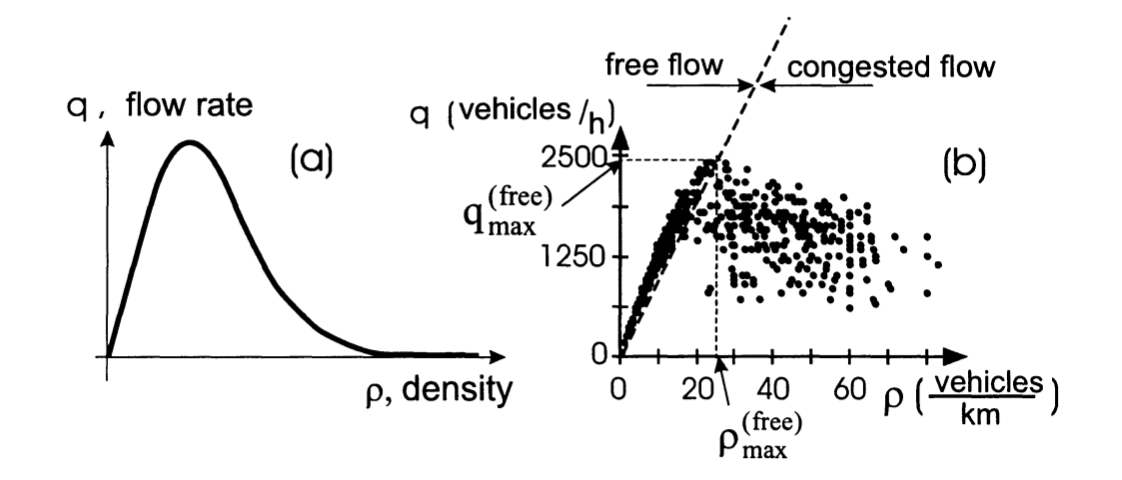
\includegraphics[width=0.65\textwidth]{Figures/Model/Kerner.png}
    \caption{$a):$ A fundamental diagram satisfying needed properties. $b):$ Observations of real patterns in different countries \cite{KernerHelbing}. }
    \label{fig:Kerner}
\end{figure} Kerner proposes to define the congested phase when the density is high enough, but also suggests dividing the congested phase into two different phases; wide-moving jams and synchronised flow \cite[p.~256]{KernerHelbing}. In this model, we will be able to explain the underlying phases of congested flow based on the behaviour of the waves of the characteristic families. This traffic model, is still inn full agreement with Kerners observations \cite{Colombo2003}.

Colombo suggests using the classical LWR model for the free phase. The argument for choosing LWR is that it gives a good solution to the problem \textit{traffic light problem} \cite[p.~71]{TrafficLight}. In this phase, the assumption is that the density $\rho$ is determined by the speed of the cars, $v(\rho)$. However, as the car density increases, the assumption that the speed is a function only on the density is no longer acceptable, and the density-flow points are scattered in a cloud rather than along a line. We denote this phase as the congested flow, see Figure \ref{fig:Kerner}b). 
%Imagine driving on a motorway, when there are few cars on the road you are free to change your velocity as you please. If you break, the car behind you will approach and the effect on the system will be an increase in density. If we instead choose to speed up, the distance between cars will increase and we have a lower density. However, when there many cars on the motorway, we are forced to reduce our speed to avoid collisions. And for a fixed density, we are allowed different speeds. A car jam can move at several different speeds, depending on factors like speed limit, the road it self, and the individual drivers. Also, different drivers tend to move at different speeds in the same velocities. We always have these few drivers who let a large portion of the road clear before picking up speed.  

Colombo proposes the following model for traffic flow: 
\begin{align}
    & \text{Free flow:}  (\rho, q) \in \Omega_f, \quad \quad \quad \text{Congested flow:} (\rho, q) \in \Omega_c, \nonumber \\
    & \rho_t + (\rho v )_x = 0, \quad \quad   \quad \quad \quad \quad 
    \begin{cases}
    \rho_t + (\rho v )_x = 0 , \\
    q_t + ((q-Q)v)_x = 0 ,
    \end{cases} \label{Eq:phase-transition} \\
    & v = v_f(\rho) = \big(1- \frac{\rho}{R}\big)V, \quad \quad \quad v = v_c(\rho,q) = \big(1 - \frac{\rho}{R}\big)\frac{q}{\rho}. \nonumber
\end{align}

Here we have the density $\rho$ and velocity $v$ as independent variables. The variable $q$ is the weighted flow, where the original motivation stems from gas dynamics, where it describes linear momentum. The two phases have different speed laws, but the maximal car density $R$, the maximal speed $V$ and the wide jam parameter $Q$ are all global and constant for the model. 

Note that the road is spatially and temporally translation invariant,  as none of the expressions depends explicitly on space or time. Thus, the model is not able to predict when or where phase transitions may appear. However, we are able to predict under which circumstances a queue forms, given the left and right states. The wave curve families, rarefaction and Hugoniot curves, will be invariant under a uniform linear scaling transformation. 
Wave curve families will be invariant under these transformations, in this case a different scaling of $\rho$ and $q$. This is useful; instead of looking at a  large family of curves, we choose one representative sample of the family and understand this, and in principle, we have understood the whole system, as the rest of the curves are just scaled versions of the representative. As a consequence of translation invariance, Colombo suggests that if initial data is contained on a single phase, it will remain in the same phase for all times. It is natural for us to first investigate the Riemann problem with initial data in the free phase, then look at the Riemann problem for the congested phase, and lastly combining the two and looking at initial data in different phases where we will experience a phase transition.

First, Colombo states a few necessary criteria in order to make the traffic flow realistic:
\begin{enumerate}
    \item The driver reacts to what is seen in front of the car, no information travels faster than cars.
    \item We cannot have a negative car density, and cars cannot travel backwards, $\rho, q \geq 0$.
    \item We have a maximal car density $R$, so that whenever a queue is formed the maximal density is reached. 
    \item Below this maximal car density, no car may stop. We are driving on a motorway until a  queue is formed. 
    \item When moving at \textit{high} car densities and speeds accelerating produce rarefaction, and breaking produce shocks. At low car density and speeds, the opposite occurs \cite{Colombo2002}. 
\end{enumerate} The criteria above will be investigated as we go through the solution of the Riemann problem for the model. 

\subsection{The Riemann Problem for Free Phase}\label{RPFreePh}
We start off by analysing the properties of the free phase, and we will at the end give the full solution for the Riemann problem for the free phase. We examine the flux function as a function of the density in a fundamental diagram, Figure \ref{Fig:Velocity function}, \ref{Fig:Flux function}. 
\begin{figure} \centering 
   \begin{minipage}{.35\textwidth}
\begin{tikzpicture}
\draw[->] (0,-0.2) -- (0,2.5);
\draw[->] (-0.2,0) -- (2.5,0);
\draw[->][magenta!70] (0,2) -- (0.8,1.2) node[anchor = south west] {$V_f$};
\draw[<-][black!50] (2,0) -- (1.2,0.8) node[anchor = south west] {$V_c$};
\draw[black!10] (2,0) -- (0.8,1.2);
%\node[magenta!70] at (1.3,1.1) {$V_f$};
\node at (2, -0.2) {$R$};
\node at (-0.2, 2) {$V$};
\node at (2.6, -0.2) {$\rho$};
\node at (-0.2, 2.6) {$v$};
\end{tikzpicture}
\caption{The velocity as a function of $\rho$.}
\label{Fig:Velocity function}
\end{minipage}
\begin{minipage}{.35\textwidth}
\begin{tikzpicture}
\draw[->] (0,-0.2) -- (0,2);
\draw[->] (-0.2,0) -- (2.5,0);
\draw[cyan!50]  plot [smooth, tension = 1.5] coordinates { (0,0) (1,1) (2,0)};
\node at (2, -0.2) {$R$};
%\node at (-0.2, 2) {$V$};
\node at (2.6, -0.2) {$\rho $};
\node at (-0.2, 2.1) {$\rho v$};
\end{tikzpicture}
\caption{The flux function in the $(\rho , \rho v)$-plane.}
\label{Fig:Flux function}
\end{minipage}
\end{figure}
Starting in $\rho = 0$, we are in the free phase. As soon as $\rho$ crosses a certain threshold $\rho_f$, we no longer regard $v$ as a function only on density, but also momentum. We call this threshold velocity, the constant $v(\rho_f) = V_f$, see Figure \ref{Fig:Velocity function}. So as $\rho$ increases in the free phase,  $v$ decreases, and reaches $V_f$. This means $V > V_f $, see Figure \ref{Fig:Velocity function}. Also, note that the flux function is concave in the $(\rho, \rho v)$-plane, see Figure \ref{Fig:Flux function}, hence we are able to invert the flux function without using convex envelopes. We have the characteristic speed $df(\rho) = \frac{d}{d\rho}(\rho v(\rho)) = V(1- \frac{2\rho}{R}) > 0$ and its clear we have a strictly hyperbolic system, and no information travels faster than the cars, the maximum velocity $V$. We have achieved criteria $1.$ for realistic traffic flow, for the free phase. This leads us to define the domain for the free phase \begin{equation}
    \Omega_f = \{(\rho, q) \in [0, \mathbb{R}] \times [0, \infty) : v_f(\rho) \geq V_f, q= \rho V \},
    \label{Domain free ph}
\end{equation} also, note that criteria $2.$ for realistic traffic flow is fulfilled, due to (\ref{Domain free ph}). 

The Riemann problem (\ref{Eq:RPFreePhase}) for the free phase, has the following solution for $(\rho_l, \rho_r) \in \Omega_f$
\begin{align}
    \rho_t + (\rho v)_x = 0,\quad  \rho(0,x) = \begin{cases} 
    \rho_l  & \text{for $x < 0$, }\\
    \rho_r  & \text{for $x \geq 0$.} 
    \end{cases}
    \label{Eq:RPFreePhase}
\end{align}

\paragraph{Shock solution.} If $\rho_l < \rho_r$, the entropy-admissible solution is a shock wave, as $f \in C^2$ and $f$ is strictly concave and thus $f'(\rho_l) > f'(\rho_r) $. The shock speed $s$ given by the Rankine-Hugoniot condition
\begin{align*}
    & \rho(x,t) = \begin{cases}
    \rho_l & \text{for $x < st$, } \\
    \rho_r & \text{for $x \geq st$, }
    \end{cases} 
    \quad \quad s = \frac{f(\rho_r) - f(\rho_l)}{\rho_r - \rho_l} = \frac{\rho_r v_f(\rho_r) -\rho_l v_f(\rho_l)}{\rho_r - \rho_l}.
\end{align*}

\paragraph{Rarefaction solution.} If $\rho_l > \rho_r$, then $f'(\rho_l) < f'(\rho_r) $ so the entropy-admissible solution is given by a rarefaction wave.
\begin{align*}
    & \rho(x,t) = \begin{cases}
    \rho_l & \text{for $x < f'(\rho_l)t$, } \\
    (f')^{-1}(x/t)  &  \text{for $ f'(\rho_l)t \leq x \geq f'(\rho_r)t$,} \\
     \rho_r & \text{for $x > f'(\rho_l)t$, }
    \end{cases} \\
    & f'(\rho) = V(1-\frac{2 \rho}{R}) , \quad  (f')^{-1}(\xi) = \frac{R}{2}(1-\frac{\xi}{V}). 
\end{align*}

We conclude this solution of the phase transition model if initial data $\rho_l, \rho_r \in \Omega_f$.

\begin{figure} \centering
    \begin{minipage}{.3\textwidth}
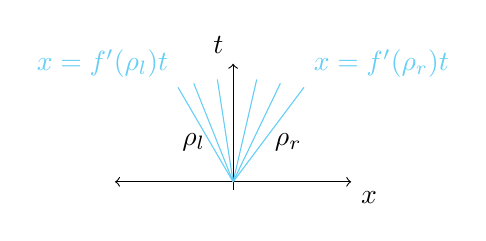
\begin{tikzpicture}
% coord.
\draw[<->] (-1.5,0) -- (1.5,0) node[anchor= north west] {$x$};
\draw[->] (0,-0.1) -- (0,1.5) node[anchor=south east] {$t$};
% rarefaction
\draw[color=cyan!60!white] (0,0) -- (0.9,1.2) node[anchor= south west] {$x = f'(\rho_r)t$};
\draw[color=cyan!60!white] (0,0) -- (0.6,1.25);
\draw[color=cyan!60!white] (0,0) -- (0.3,1.3);
\draw[color=cyan!60!white] (0,0) -- (-0.2,1.3);
\draw[color=cyan!60!white] (0,0) -- (-0.5,1.25);
\draw[color=cyan!60!white] (0,0) -- (-0.7,1.2) node[anchor= south east] {$x = f'(\rho_l)t$};
\node at (-0.5, 0.5) {$\rho_l$};
\node at (0.7, 0.5) {$\rho_r$};
\end{tikzpicture}
\caption{The solution to the Riemann problem, $\rho_l < \rho_r$.}
\label{Fig: SolRP_raref_disc}
\end{minipage}
\quad \quad \quad \quad \quad \quad \quad \quad
\begin{minipage}{.3\textwidth}
\begin{tikzpicture}
\draw[<->] (-1.5,0) -- (1.5,0) node[anchor= north west] {$x$};
\draw[->] (0,-0.1) -- (0,1.5) node[anchor=south east] {$t$};
\draw[color=cyan!90!white] (0,0) -- (0.9,1.2) node[anchor= south west] {$x = st$};
\node at (-0.5, 0.5) {$\rho_l$};
\node at (0.7, 0.5) {$\rho_r$};
\end{tikzpicture}
\caption{The solution to the Riemann problem, $\rho_l < \rho_r$.}
\label{Fig: SolRP_shock_disc}
\end{minipage}
\end{figure}

\begin{figure}
     \centering
     \begin{subfigure}[b]{0.3\textwidth}
         \centering
         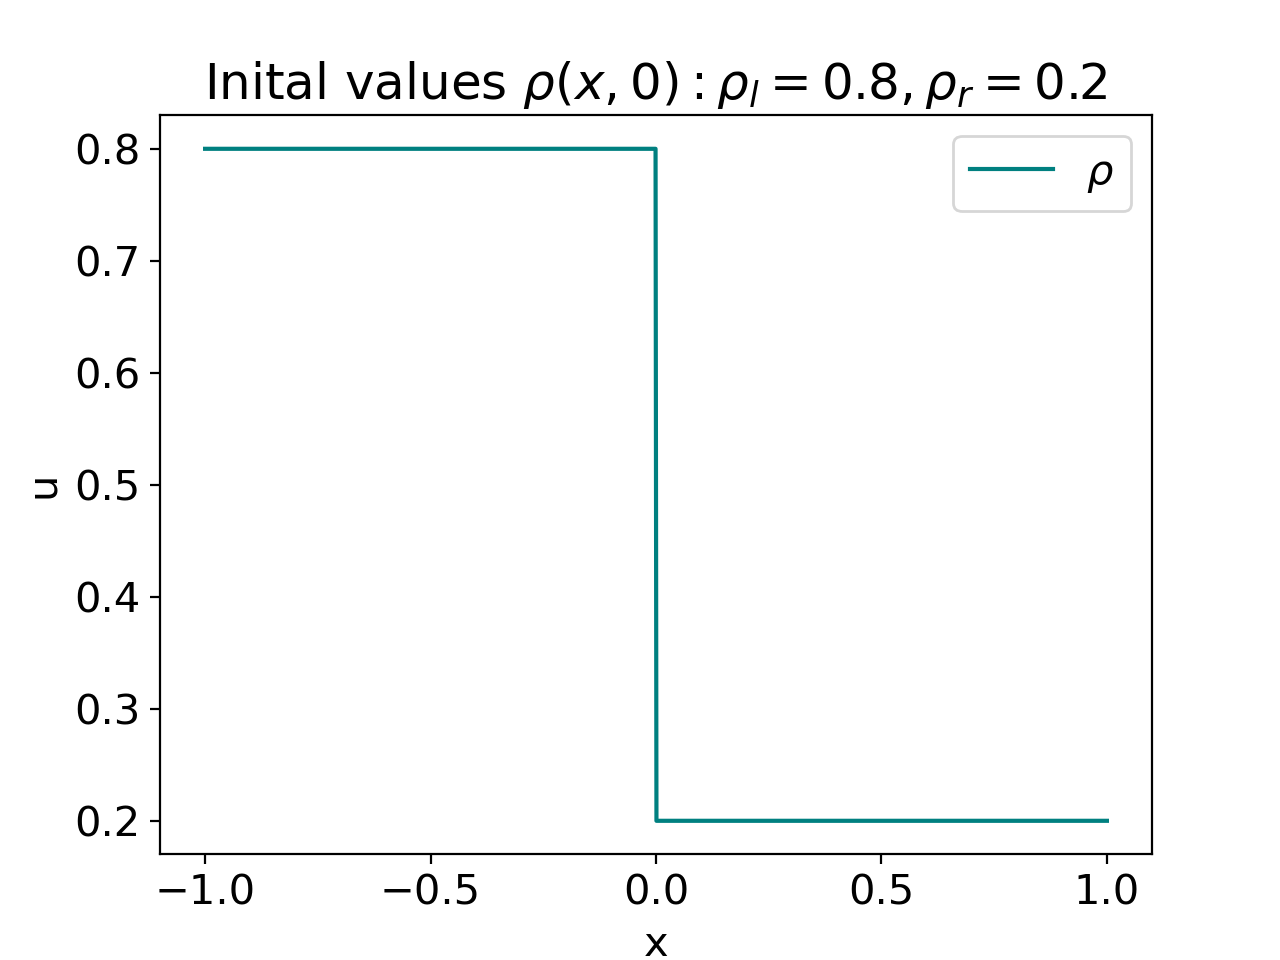
\includegraphics[width=\textwidth]{Figures/Model/RarefacIV.png}
         %\caption{Initial value plot.}
         %\label{fig:RarefacIV}
     \end{subfigure}
     \hfill
     \begin{subfigure}[b]{0.3\textwidth}
         \centering
         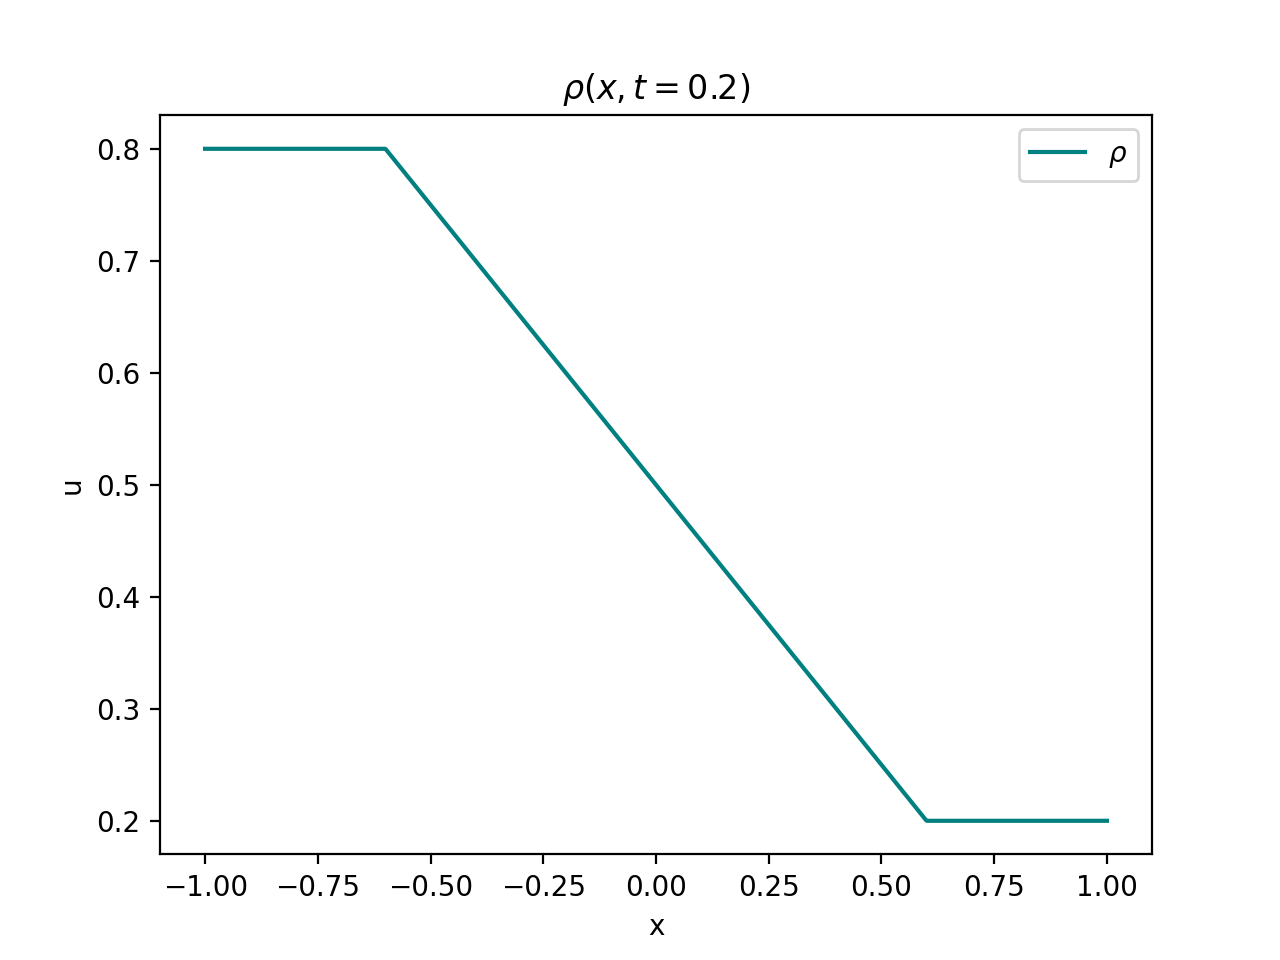
\includegraphics[width=\textwidth]{Figures/Model/RarefacAtTime.png}
         %\caption{Solution $\rho(x,t)$ at time $t = 0.2$}
         %\label{fig:RarefacAtTime}
     \end{subfigure}
     \hfill
     \begin{subfigure}[b]{0.3\textwidth}
         \centering
         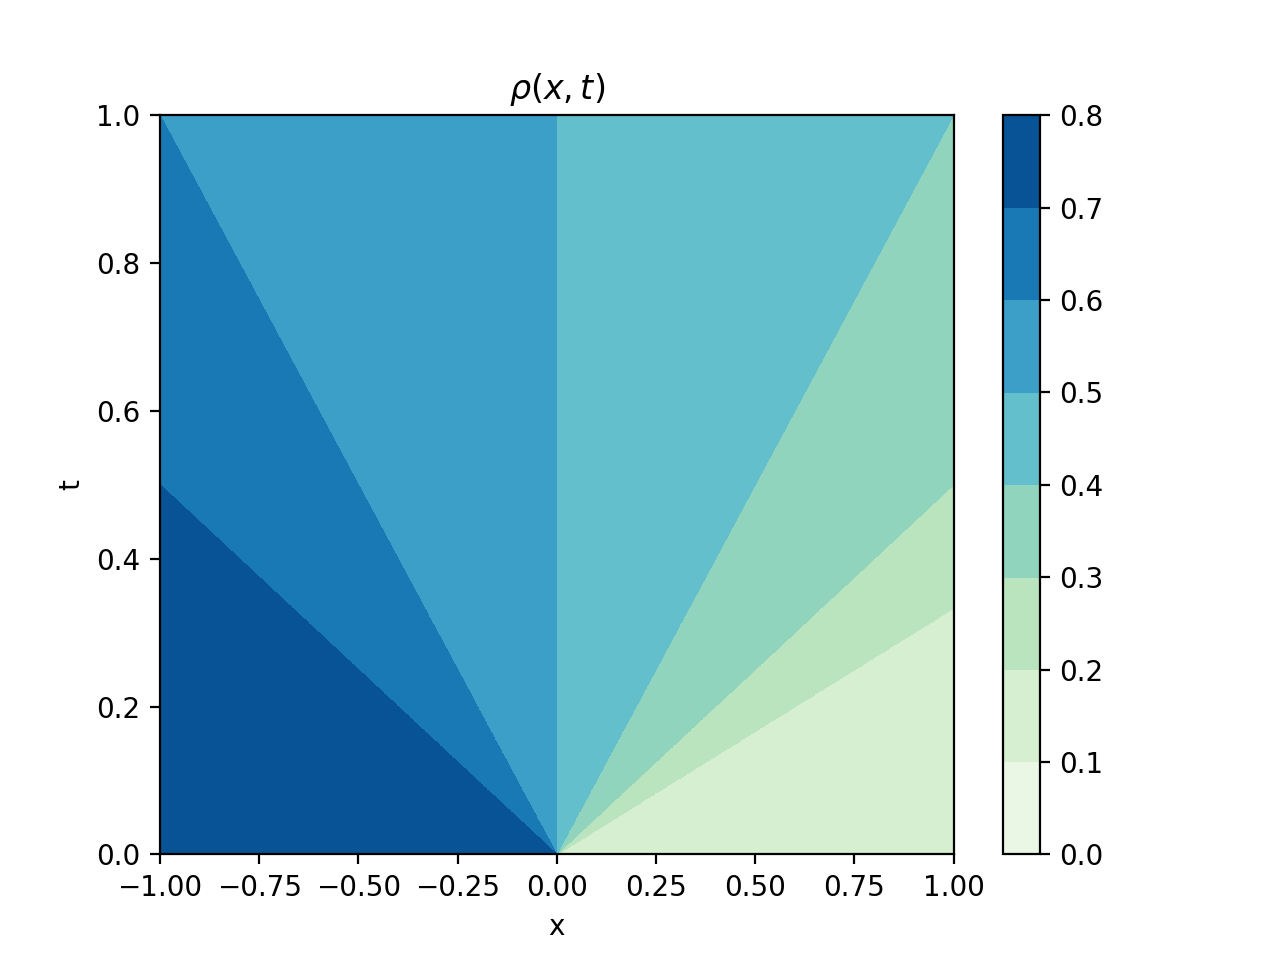
\includegraphics[width=\textwidth]{Figures/Model/RarefactionFull.png}
         %\caption{The solution $\rho$ in the $x,t$-plane. }
         %\label{fig:five over x}
     \end{subfigure}
        \caption{The evolution of a solution with initial values $\rho_l = 0.8, \rho_r = 0.2$, seen to the left. After $t = 0.2$, we have the middle figure. A full solution in the $x,t$-plane can be seen to the right.}
        \label{fig:ExampleRarefaction}
\end{figure}

\subsection{The Riemann Problem for the Congested phase}\label{RPCongPh}

When the $\rho$ increases and velocity $v$ reaches the constant threshold $v(\check R) = V_c$, see Figure \ref{Fig:Velocity function}, the traffic enters the congested phase. Now we have the relation $ V > V_f > V_c $, and we define the domain for the congested phase as follows \begin{equation}
    \Omega_c = \Bigg\{(\rho, q) \in [0, \mathbb{R}] \times [0, \infty) : v_c(\rho, q) \leq V_c, \frac{q-Q}{\rho} \in \Bigg[\frac{Q_1 - Q}{R}, \frac{Q_2 - Q}{R} \Bigg]  \Bigg\},
    \label{Domain congested ph}
\end{equation} again note that with this definition criteria $2.$ and $3.$ are fulfilled for the congested phase. 
\begin{wrapfigure}[10]{l}{0.3\textwidth}
    \begin{center}
        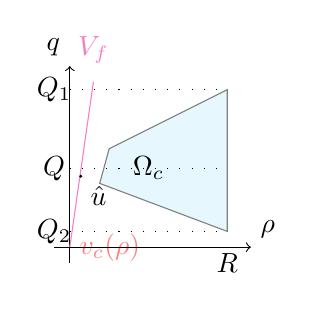
\begin{tikzpicture}
        % coordinates
        \draw[->] (0,-0.2) -- (0,2.3) node[anchor=south east] {$q$};
        \draw[red!50, domain=0:0.7]  plot[id=x] function{x*(3*x+1)}  node[right] {$v_c(\rho)$};
        \draw[magenta!50] (0,0) -- (0.3,2.1);
        \node[magenta!50] at (0.3,2.5) {$V_f$};
        \filldraw[black] (0.14,0.9) circle (0.3pt) node[anchor = north west]{$\hat u$} ;
         \filldraw[fill=cyan!10!white, draw=black!50] plot [tension = 1] coordinates { (0.5,1.25) (2,2) (2,0.2) (0.38, 0.81) (0.5,1.25)};
         \node at (1,1) {$\Omega_c$};
         \draw[->] (-0.2,0) -- (2.3,0) node[anchor=south west] {$\rho$};
        \node at (2,-0.2) {$R$};
         \node at (-0.2,2) {$Q_1$};
         \node at (-0.2,0.2) {$Q_2$};
         \node at (-0.2,1) {$Q$};
         \draw[loosely dotted] (0,1) -- (2,1);
         \draw[loosely dotted] (0,2) -- (2,2);
         \draw[loosely dotted] (0,0.2) -- (2,0.2);
       \end{tikzpicture}
    \caption{Domain  $\Omega_c$}
    \label{fig:ConservationLaws/I}
    \end{center}
\end{wrapfigure}{}
Where $Q_1$ and $Q_2$ determines the width of the domain $\Omega_{c}$, or the "cloud" in the congested phase \cite{Colombo2003}. Note $V_f > V_c$, as if $V_f = V_c$ the Riemann problem is not well-posed. We will return to this issue in the solution of the full model. Let $ u = (\rho, q)$, and we write the equations on system form

\begin{align*}
    \underbrace{\begin{pmatrix} \rho \\ q \end{pmatrix}_t}_{u_t} +  \underbrace{\begin{pmatrix} \rho v  \\ (q - Q) v \end{pmatrix}_x}_{f(u)_x} = 0, 
\end{align*}

where $v = v_c(\rho,  q) = (1 - \frac{\rho}{R}) \frac{q}{\rho}$. The system has the following Jacobian:

\begin{equation*}
    df(u) =\begin{pmatrix} -\frac{q}{R} & (1- \frac{\rho}{R}) \\ 
                            \frac{q(Q-q)}{\rho ^2} & \quad (2q -Q)(\frac{1}{\rho} - \frac{1}{R}) \end{pmatrix}.
\end{equation*}

When finding the eigenvalues $\lambda_i$ (\ref{Eq:EigenvaluesCongestedPhase}) and eigenvectors $r_i$ (\ref{Eq:EigenvectorsCongPh}), we see we have a strictly hyperbolic system with $\lambda_1 < \lambda_2 = v_c$ as long as $\rho > 0, q, R \geq 0$, and we have achieved both criteria $1. $ and $2.$ for realistic traffic flow.  Also in this phase, no information travels faster than the cars. 
\begin{align}
    &\lambda_1 = \big ( \frac{2}{R} - \frac{1}{\rho} )\big (Q- q) - \frac{Q}{R} , \quad \quad \lambda_2 = \big(1 - \frac{\rho}{q}\big)\frac{q}{\rho} = v_c , \label{Eq:EigenvaluesCongestedPhase} \\
    & r_1 = \begin{pmatrix} \rho \\ q - Q \end{pmatrix}, \quad \quad \quad  \quad \quad \quad \quad \quad  r_2 = \begin{pmatrix} R - \rho \\ \frac{Rq}{\rho} \end{pmatrix} , \label{Eq:EigenvectorsCongPh} \\
    & \nabla \lambda_1 \cdot r_1 = 2\frac{Q-q}{R}, \quad \quad \quad \quad \quad  \quad \nabla \lambda_2 \cdot r_2 = 0 . \label{Eq:GNLorLDcongPh}
\end{align}
When investigating (\ref{Eq:GNLorLDcongPh}) we see that if $q \neq Q$ we have one genuinely non-linear first family and one linearly degenerate second family. However, if $ Q = q$, we have a linearly degenerate field also for the first wave. So the first wave is both genuinely non-linear and linearly degenerate. However, this will not be a problem as we will see later.

\paragraph{Rarefaction curves and contact discontinuities.}
We continue by finding the wave curves for the genuinely non-linear case of the first family, we denote this rarefaction curve $q_1$. For the linearly degenerate second family we find a contact discontinuity, and denote it $q_2$. We assume $u_l$ is fixed and integrate the eigenvectors from $u_l$ to $u$ in the phase-plane. This leads to the following wave curves
\begin{align}
    & q_1 = \frac{q_l - Q}{\rho_l} \rho + Q, \quad \quad \textit{Rarefaction curve,}
    \label{Eq:RarefactionWCongestedPh} \\
    &  q_2 = \frac{q_l}{\rho_l} \frac{R - \rho_l}{R- \rho} \rho,   \quad \quad \textit{Contact Discontinuity.}
    \label{Eq:ContactDiscCongestedPh}
\end{align}

\paragraph{Shock curves.}
Lastly, using the Rankine-Hugoniot condition (\ref{Hugoniot_locus}), and solving for $q$ by eliminating $s$, and inserting for $v = v_c = (1- \frac{\rho}{R})\frac{q}{\rho}$ we find
\begin{align}
     s \begin{pmatrix} \rho_l - \rho \\ q_l - q \end{pmatrix} &= \begin{pmatrix} \rho_l v_l - \rho v \\ (q_l - Q)v_l - (q - Q)v \end{pmatrix} \nonumber\\
     \frac{\rho v - \rho_l v_l}{\rho - \rho_l} &= \frac{(q-Q)v - (q_l-Q)v_l}{q - q_l} \nonumber\\
      q &= \frac{q_l - Q}{\rho_l} \rho + Q,  \quad \quad \textit{Shock curve.}
     \label{Eq:ShockCongPh}
\end{align}
We find the rarefaction curve (\ref{Eq:RarefactionWCongestedPh}) and shock curve (\ref{Eq:ShockCongPh}) coincides for the first family, and together with the contact discontinuity (\ref{Eq:ContactDiscCongestedPh}) we only have two solution curves in the phase-plane for the congested phase. In the $(\rho,q)$-plane the $1$-family are straight lines, while the $2$-family are convex.
We still do not know the direction of the first family, and we still have both a shock and a rarefaction solution along the first wave family, and hence we continue with Lax entropy. 

\paragraph{Lax entropy.}
%\begin{align*}
%    & q > Q \implies \nabla \lambda_1 \cdot r_1 < 0 \\
%    & q < Q \implies \nabla \lambda_1 \cdot r_1 > 0
%\end{align*}
We wish to find how $\lambda$ changes on the first wave, as increasing $\lambda$ is a requirement for Lax entropy. The first wave can be rewritten as 
\begin{align*}
q &=  \frac{\rho( q_l - Q)}{\rho_l} + Q \\
 & \frac{\rho( q - Q)}{\rho}  =  \frac{\rho( q_l - Q)}{\rho_l}.
\end{align*}
Inserting this expression for the first wave into the expression for $\lambda_1$, we have
\begin{align}
     \lambda_1 &= \big ( \frac{2}{R} - \frac{1}{\rho} )\big (Q- q) - \frac{Q}{R} 
     = \frac{Q - 2q}{R} + \frac{q-Q}{\rho} \nonumber \\
     \lambda_1 &= \frac{Q - 2q}{R} + \frac{q_l-Q}{\rho_l}.
     \label{Eq:DirectionOfLambda}
\end{align}

Using the Lax entropy condition for the shock wave, along with the found direction of increasing $\lambda$ we have \begin{align}
   &  \lambda_1 (u_r) < s < \lambda_1 (u_l).
   \label{Eq:LaxEntropyCongPh}
\end{align} We need an increase in $\lambda_1 $ from $u_r$ to $u_l$ to have a Lax 1-shock.

\begin{figure}
    \centering
    \begin{minipage}{.35\textwidth}
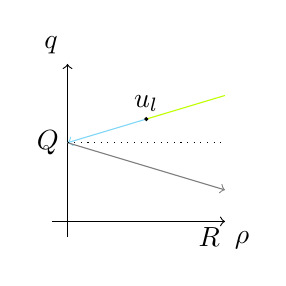
\begin{tikzpicture}
% coordinates
\draw[->] (0,-0.2) -- (0,2) node[anchor= south east] {$q$};
\draw[->] (-0.2,0) -- (2,0) node[anchor= north west] {$\rho$};
% rarefactions

\draw[lime] (1, 1.3) -- (2, 1.6) ;
\draw[<-][cyan!50] (0, 1) -- (1, 1.3) ;
\draw[->][black!50] (0, 1) -- (2, 0.4) ;
\draw[dotted] (0,1) -- (2, 1);
\filldraw[black] (1,1.3) circle (0.5pt) ;
\node at (1, 1.5) {$u_l$};
\node at (1.8, -0.2) {$R$};
\node at (-0.25, 1) {$Q$};
\end{tikzpicture}
\caption{Lax entropy for $q > Q$. \\ Rarefaction (blue) and \\shock (green).}
\label{Fig:LaxEntropy1CongestedPhase}
\end{minipage}
\quad \quad \quad \quad 
\begin{minipage}{.35\textwidth}
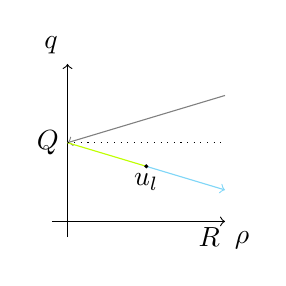
\begin{tikzpicture}
% coordinates
\draw[->] (0,-0.2) -- (0,2) node[anchor= south east] {$q$};
\draw[->] (-0.2,0) -- (2,0) node[anchor= north west] {$\rho$};
% rarefactions
\draw[<-][black!50] (0, 1) -- (2, 1.6) ;
\draw[->][cyan!50] (1,0.7) -- (2, 0.4) ;
\draw[-][lime] (0, 1) -- (1,0.7) ;
\draw[dotted] (0,1) -- (2, 1);
\filldraw[black] (1,0.7) circle (0.5pt) ;
\node at (1, 0.5) {$u_l$};
\node at (1.8, -0.2) {$R$};
\node at (-0.25, 1) {$Q$};
\end{tikzpicture}
\caption{Lax entropy for $q < Q$ \\ Rarefaction (blue) and \\shock (green).}
\label{Fig:LaxEntropy2CongestedPhase}
\end{minipage}
\end{figure}

Now, investigating what happens above the critical line $ q = Q$, see Figure \ref{Fig:LaxEntropy1CongestedPhase}. Due to the direction of $\lambda_1$ in combination with (\ref{Eq:LaxEntropyCongPh}) we get a shock when moving backwards from $u_l$. That means, when $q > Q$ , $\rho_l < \rho_r$ produce a shock, and $\rho_l > \rho_r$ produce a rarefaction . Below the critical line $q < Q$, see Figure \ref{Fig:LaxEntropy2CongestedPhase}, by applying the same argument we also get a shock moving backwards from $u_l$. That means, when $q < Q$ , $\rho_l < \rho_r$ produce a rarefaction, and $\rho_l > \rho_r$ produce a shock .The regions for shock and rarefaction on the first family wave curves are depicted in both figures, as well as the direction of increasing $\lambda_1$. Colombo summarised this result nicely in \cite{Colombo2002}.
\begin{equation}
\begin{aligned}
   & \begin{cases}
    \nabla \lambda_1 \cdot r_1 < 0 , \\
    q > Q ,
    \end{cases} \iff \begin{cases}
    \text{Braking} \leftrightarrow \text{Shock,} \\
    \text{Accelerating} \leftrightarrow \text{Rarefaction,} 
    \end{cases}  \\
   &\begin{cases}
    \nabla \lambda_1 \cdot r_1 > 0 , \\
    q < Q ,
    \end{cases} \iff \begin{cases}
    \text{Braking} \leftrightarrow \text{Rarefaction,} \\
    \text{Accelerating} \leftrightarrow \text{Shock,} 
    \end{cases}
    \label{LaxentropySummarised}
\end{aligned} \end{equation} From the result above (\ref{LaxentropySummarised}), we have now acquired criteria $5.$ for realistic traffic flow, and it is allowed by the $(q-Q)v$-term in the model equation for congested traffic. 
%From an experimental point of view we can now estimate the parameters $Q_1, Q_2$, and $Q$. 
%We can also reformulate the solution curves in the $(\rho, \rho v)$-plane, for both the congested phase and free phase. 
\paragraph{The Riemann Problem.}
We have now all the necessary components to solve the Riemann Problem in the congested phase. Assume $(u_l, u_r) \in \Omega_c, u = (\rho, q)$, we have the following Riemann problem: 
\begin{align}
     \begin{cases} \rho_t + (\rho v)_x = 0 \\
     q_t + ((q-Q)v)_x = 0 ,
    \end{cases} \quad \quad (\rho, q) (0,x) = \begin{cases}
    (\rho_l, q_l) & \text{for $x < 0$,} \\
    (\rho_r, q_r) &  \text{for $x \geq 0$,}
    \end{cases}
    \label{Eq:RPCongestedPhase}
\end{align}

We have two wave curve families. The first and slow family $W_1(u_l)$, 
\begin{align*}
     W_1(u_l) = \frac{\rho( q_l - Q)}{\rho_l} + Q  \begin{cases}
          q_l > Q:  \text{Rarefaction when $\rho_l > \rho_r$, shock when $\rho_l < \rho_r$,}\\
          q_l < Q: \text{Rarefaction when $\rho_l < \rho_r$ shock when $\rho_l > \rho_r$,} \\
          q_l = Q:  \text{Contact discontinuity for all $\rho_l, \rho_r$. } \
     \end{cases}
\end{align*}
And the second fast family 
\begin{align*}
     W_2(u_l) = \frac{\rho( R - \rho_l)}{\rho_l( R - \rho)}, \quad \text{Contact discontinuity for all $u$.}
\end{align*}

We always have to move in the direction of increasing $\lambda$, this makes us travel from left state along the slow wave to a middle state, followed by a fast wave to the right state. If $u_l, u_r \in W_1(u_l)$ then the solution is only a slow first wave $W_1(u_l)$ to $u_r$, for shock, rarefaction and contact discontinuity if $u_l(\rho, q_l = Q)$. This also holds for $u_l, u_r \in W_2(u_l)$, then the solution is only a fast second family wave from $u_l$ to $u_r$. 

We have proved Proposition $2.1$ in \cite{Colombo2002}. We state the result below.

\begin{proposition}
Fix positive $Q, R, V$, and let $\rho > 0$ . For all $(\rho_l, q_l)$ and $(\rho_r, q_r)$ in $\Omega_c$, the Riemann problem (\ref{Eq:RPCongestedPhase}) with \begin{align*}
    v = v_c(\rho,q) = \big(1 - \frac{\rho}{R}\big)\frac{q}{\rho},
\end{align*} admits a unique self-similar solution consisting of a slow wave $W_1(u_l)$ between  $(\rho_l, q_l)$ and  $(\rho_m, q_m)$, followed by a fast contact discontinuity  $W_2(u_m)$ between  $(\rho_m, q_m)$ and  $(\rho_r, q_r)$. The slow wave is present whenever $v_c(\rho_l, q_l) \neq v_c(\rho_r, q_r)$ and is either a shock, rarefaction or a contact discontinuity. The latter case if and only if $q_l = Q$. In all cases, the solution attains values in $\Omega_c$.
\end{proposition}
Note we require $\rho > 0$ for well-posedness, as the contact discontinuity is undefined for $\rho = 0$. However, this will not be a problem when investigating the full model, as a phase-transition into a free phase will occur when we approach low density. 

\begin{figure} \centering
    \begin{minipage}{.3\textwidth}
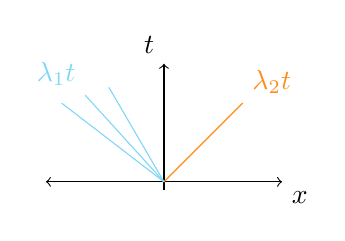
\begin{tikzpicture}
% coord.
\draw[<->] (-1.5,0) -- (1.5,0) node[anchor= north west] {$x$};
\draw[->] (0,-0.1) -- (0,1.5) node[anchor=south east] {$t$};
% contact disc
\draw[color=orange!90!white] (0,0) -- (1,1) node[anchor= south west] {$\lambda_2 t$};
% rarefaction
\draw[color=cyan!50!white] (0,0) -- (-1.3,1);
\draw[color=cyan!50!white] (0,0) -- (-1,1.1) node[anchor= south east] {$\lambda_1 t$};
\draw[color=cyan!50!white] (0,0) -- (-0.7,1.2);
\end{tikzpicture}
\caption{Slow rarefaction (blue) followed by a contact discontinuity (orange).}
\label{Fig:SolRPRarefDiscCongestedPhase}
\end{minipage}
\quad \quad
\begin{minipage}{.3\textwidth}
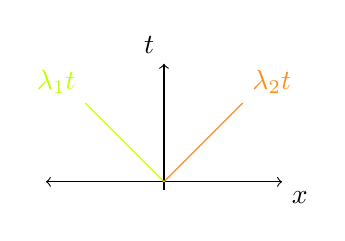
\begin{tikzpicture}
\draw[<->] (-1.5,0) -- (1.5,0) node[anchor= north west] {$x$};
\draw[->] (0,-0.1) -- (0,1.5) node[anchor=south east] {$t$};
\draw[color=orange!90!white] (0,0) -- (1,1) node[anchor= south west] {$\lambda_2 t$};
\draw[color=lime] (0,0) -- (-1,1) node[anchor= south east] {$\lambda_1 t$};
\end{tikzpicture}
\caption{Slow shock (green) followed by a contact discontinuity (orange).}
\label{Fig:SolRPShockDiskCongestedPhase}
\end{minipage}
\quad 
\begin{minipage}{.3\textwidth}
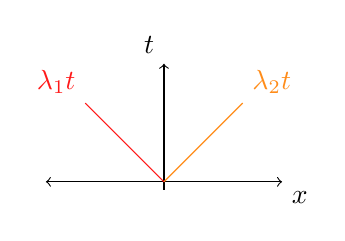
\begin{tikzpicture}
\draw[<->] (-1.5,0) -- (1.5,0) node[anchor= north west] {$x$};
\draw[->] (0,-0.1) -- (0,1.5) node[anchor=south east] {$t$};
\draw[color=orange!90!white] (0,0) -- (1,1) node[anchor= south west] {$\lambda_2 t$};
\draw[color=red!90!white] (0,0) -- (-1,1) node[anchor= south east] {$\lambda_1 t$};
\end{tikzpicture}
\caption{Contact discontinuity followed by a contact discontinuity, $q_l = Q$.}
\label{Fig:SolRPDiscCongestedPhase}
\end{minipage}
\end{figure}

We will now demonstrate possible solutions of (\ref{Eq:RPCongestedPhase}). The combinations of waves in the $(x,t)$-plane can be seen in Figures \ref{Fig:SolRPRarefDiscCongestedPhase}, \ref{Fig:SolRPShockDiskCongestedPhase} and \ref{Fig:SolRPDiscCongestedPhase}, note the order of the first and second family waves are consistent with previous results. Figure \ref{fig:SolRPCongInRhoQ} shows four possible solutions in $\Omega_c$. The corresponding written solutions are (\ref{Eq:correspondingSolu1u2}), (\ref{Eq:correspondingSolu3u4}). 
\begin{figure}
    \centering
    \begin{minipage}{.2\textwidth}
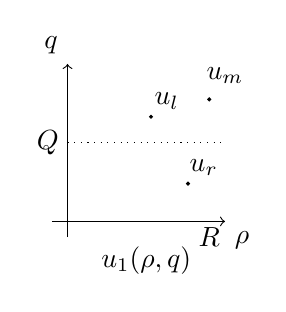
\begin{tikzpicture}
% coordinates
\draw[->] (0,-0.2) -- (0,2) node[anchor= south east] {$q$};
\draw[->] (-0.2,0) -- (2,0) node[anchor= north west] {$\rho$};
% rarefactions
%\draw[cyan!50] (1, 1.3) -- (2, 1.6) ;
%\draw[<-][lime] (0, 1) -- (1, 1.3) ;
%\draw[->][cyan!50] (0, 1) -- (2, 0.4) ;


\draw[lime, domain=0:2]  plot[id=x] function{0.31*x +1};
\draw[black!30, domain=0:2]  plot[id=x] function{-0.34*x +1};
\draw[dotted] (0,1) -- (2, 1);
% contact disk
\draw[black!30, domain=0:1.28]  plot[id=x] function{(x/1.16)*(2-1.16)/(2-x)*1.63};
\draw[orange!50, domain=0:1.86]  plot[id=x] function{(x/1.38)*(2-1.38)/(2-x)*0.33};
% initial conditions
\node at (1.06+0.2, 1.33+0.2) {$u_l$};
\node at (1.53+0.2, 0.48+0.2) {$u_r$};
\node at (1.8+0.2, 1.55+0.3) {$u_m$};
\filldraw[black] (1.06, 1.33) circle (0.5pt);  % u_1
\filldraw[black] (1.53, 0.48) circle (0.5pt);   % u_2
\filldraw[black] (1.8, 1.55) circle (0.5pt);   % u_m
%labels
\node at (1.8, -0.2) {$R$};
\node at (-0.25, 1) {$Q$};
\node at (1, -0.5) {$u_1(\rho, q)$};
\end{tikzpicture}
\end{minipage}
\begin{minipage}{.2\textwidth}
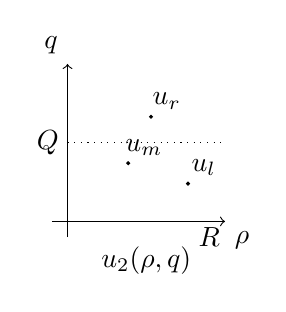
\begin{tikzpicture}
% coordinates
\draw[->] (0,-0.2) -- (0,2) node[anchor= south east] {$q$};
\draw[->] (-0.2,0) -- (2,0) node[anchor= north west] {$\rho$};
% rarefactions
%\draw[cyan!50] (1, 1.3) -- (2, 1.6) ;
%\draw[<-][lime] (0, 1) -- (1, 1.3) ;
%\draw[->][cyan!50] (0, 1) -- (2, 0.4) ;
\draw[black!30, domain=0:2]  plot[id=x] function{0.31*x +1};
\draw[lime, domain=0:2]  plot[id=x] function{-0.34*x +1};
\draw[dotted] (0,1) -- (2, 1);
% contact disk
\draw[orange!50, domain=0:1.28]  plot[id=x] function{(x/1.16)*(2-1.16)/(2-x)*1.63};
\draw[black!30, domain=0:1.86]  plot[id=x] function{(x/1.38)*(2-1.38)/(2-x)*0.33};
% initial conditions
\node at (1.06+0.2, 1.33+0.2) {$u_r$};
\node at (1.53+0.2, 0.48+0.2) {$u_l$};
\node at (0.77+0.2, 0.74+0.2) {$u_m$};
\filldraw[black] (0.77, 0.74) circle (0.5pt);   % u_m
\filldraw[black] (1.06, 1.33) circle (0.5pt);  % u_1
\filldraw[black] (1.53, 0.48) circle (0.5pt);   % u_2
%labels
\node at (1.8, -0.2) {$R$};
\node at (-0.25, 1) {$Q$};
\node at (1, -0.5) {$u_2(\rho,q)$};
\end{tikzpicture}
\end{minipage}
\quad
\begin{minipage}{.2\textwidth}
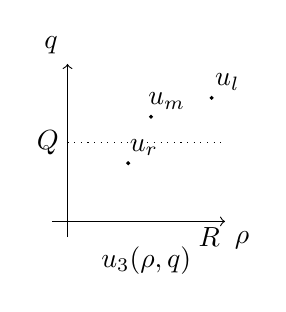
\begin{tikzpicture}
% coordinates
\draw[->] (0,-0.2) -- (0,2) node[anchor= south east] {$q$};
\draw[->] (-0.2,0) -- (2,0) node[anchor= north west] {$\rho$};
% rarefactions
%\draw[cyan!50] (1, 1.3) -- (2, 1.6) ;
%\draw[<-][lime] (0, 1) -- (1, 1.3) ;
%\draw[->][cyan!50] (0, 1) -- (2, 0.4) ;
\draw[cyan!50, domain=0:2]  plot[id=x] function{0.31*x +1};
\draw[black!30, domain=0:2]  plot[id=x] function{-0.34*x +1};
\draw[dotted] (0,1) -- (2, 1);
% contact disk
\draw[orange!50, domain=0:1.28]  plot[id=x] function{(x/1.16)*(2-1.16)/(2-x)*1.63};
\draw[black!30, domain=0:1.86]  plot[id=x] function{(x/1.38)*(2-1.38)/(2-x)*0.33};
% initial conditions
\node at (1.83+0.2, 1.57+0.2) {$u_l$};
\node at (0.77+0.2, 0.74+0.2) {$u_r$};
\node at (1.06+0.2, 1.33+0.2) {$u_m$};
\filldraw[black] (1.83, 1.57) circle (0.5pt);  % u_1
\filldraw[black] (0.77, 0.74) circle (0.5pt);   % u_2
\filldraw[black] (1.06, 1.33) circle (0.5pt);  % u_m
%labels
\node at (1.8, -0.2) {$R$};
\node at (-0.25, 1) {$Q$};
\node at (1, -0.5) {$u_3(\rho,q)$};
\end{tikzpicture}
\end{minipage}
\begin{minipage}{.2\textwidth}
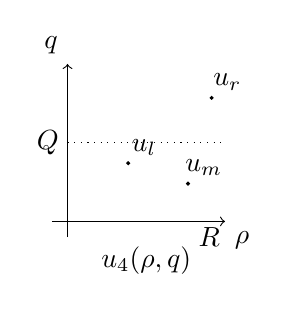
\begin{tikzpicture}
% coordinates
\draw[->] (0,-0.2) -- (0,2) node[anchor= south east] {$q$};
\draw[->] (-0.2,0) -- (2,0) node[anchor= north west] {$\rho$};
% rarefactions
%\draw[cyan!50] (1, 1.3) -- (2, 1.6) ;
%\draw[<-][lime] (0, 1) -- (1, 1.3) ;
%\draw[->][cyan!50] (0, 1) -- (2, 0.4) ;
\draw[black!30, domain=0:2]  plot[id=x] function{0.31*x +1};
\draw[cyan!50, domain=0:2]  plot[id=x] function{-0.34*x +1};
\draw[dotted] (0,1) -- (2, 1);
% contact disk
\draw[black!30, domain=0:1.28]  plot[id=x] function{(x/1.16)*(2-1.16)/(2-x)*1.63};
\draw[orange!50, domain=0:1.86]  plot[id=x] function{(x/1.38)*(2-1.38)/(2-x)*0.33};
% initial conditions
\node at (1.83+0.2, 1.57+0.2) {$u_r$};
\node at (0.77+0.2, 0.74+0.2) {$u_l$};
\node at (1.53+0.2, 0.48+0.2) {$u_m$};
\filldraw[black] (1.83, 1.57) circle (0.5pt);  % u_1
\filldraw[black] (0.77, 0.74) circle (0.5pt);   % u_2
\filldraw[black] (1.53, 0.48) circle (0.5pt);  % u_m
%labels
\node at (1.8, -0.2) {$R$};
\node at (-0.25, 1) {$Q$};
\node at (1, -0.5) {$u_4(\rho, q)$};
\end{tikzpicture}
\end{minipage}
    \caption{Solutions of the congested phase in the $(\rho,q)$-plane. All solution curves emanating for the points $u_l, u_r$ are drawn, but only the coloured are admissible solutions. Rarefactions (blue), shocks (green) and contacts (orange). }
    \label{fig:SolRPCongInRhoQ}
\end{figure}
\begin{align}
    u_1(x,t) = \begin{cases} 
    u_l & \text{for  $x < \lambda_1(u_l)t$},\\
    %W_1, \lambda_1(u_l)t < x < \lambda_1(u_r)t, \quad \textit{Shock}\\ 
    u_m & \text{for $\lambda_1(u_r)t < x < \lambda_2(u_l)t$}, \\
    %W_2, \lambda_2(u_l)t < x < \lambda_2(u_r)t \quad \textit{Contact D.} \\
    u_r & \text{for $ x > \lambda_2(u_r)t$}, \\
    \end{cases} \quad
    u_2(x,t) = \begin{cases}
    u_l & \text{for $ x < \lambda_1(u_l)t$},\\
    %W_1, \lambda_1(u_l)t < x < \lambda_1(u_r)t, \quad \textit{Shock}\\ 
    u_m & \text{for $ \lambda_1(u_r)t < x < \lambda_2(u_l)t$}, \\
    %W_2, \lambda_2(u_l)t < x < \lambda_2(u_r)t \quad \textit{Contact D.} \\
    u_r & \text{for $ x > \lambda_2(u_r)t$}, \\
    \end{cases}
    \label{Eq:correspondingSolu1u2}
\end{align}
\begin{align}
    u_3(x,t) = \begin{cases}
    u_l  &\text{ for $x < \lambda_1(u_l)t$},\\
    w_1 &\text{ for $ \lambda_1(u_l)t < x < \lambda_1(u_r)t$},\\ 
    u_m &\text{for  $\lambda_1(u_r)t < x < \lambda_2(u_l)t$}, \\
   % W_2, \lambda_2(u_l)t < x < \lambda_2(u_r)t \quad \textit{Contact D.} \\
    u_r &\text{for  $x > \lambda_2(u_r)t$}, \\
    \end{cases} \quad 
    u_4(x,t) = \begin{cases}
    u_l  &\text{for $x < \lambda_1(u_l)t$},\\
    w_1 &\text{for $\lambda_1(u_l)t < x < \lambda_1(u_r)t$}, \\ 
    u_m  &\text{for $\lambda_1(u_r)t < x < \lambda_2(u_l)t$}, \\
   % W_2, \lambda_2(u_l)t < x < \lambda_2(u_r)t \quad \textit{Contact D.} \\
    u_r  &\text{for $x > \lambda_2(u_r)t$},
    \label{Eq:correspondingSolu3u4}
    \end{cases}
\end{align}
\begin{align}
    u_5(x,t) = \begin{cases}
    u_l & \text{for $x < \lambda_1(u_l)t$},\\
    %W_1, \lambda_1(u_l)t < x < \lambda_1(u_r)t, \quad \textit{Contact D.}\\ 
    u_m & \text{for $\lambda_1(u_r)t < x < \lambda_2(u_l)t$}, \\
    %W_2, \lambda_2(u_l)t < x < \lambda_2(u_r)t \quad \textit{Contact D.} \\
    u_r & \text{for $x> \lambda_2(u_r)t$,} \\
    \end{cases}
    \label{Eq:u_5}
\end{align}
\begin{align*}
   & \lambda_1(u_l) = .. , \quad \lambda_2(u_l) = \lambda_2(u_r) = ... \\
   & w_1 = . . .
\end{align*}

\begin{wrapfigure}[11]{r}{0.29\textwidth}
    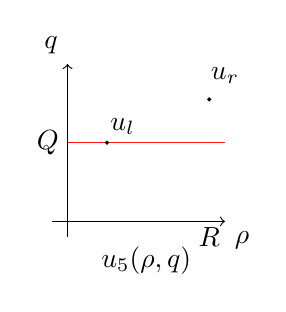
\begin{tikzpicture}
    % coordinates
    \draw[->] (0,-0.2) -- (0,2) node[anchor= south east] {$q$};
    \draw[->] (-0.2,0) -- (2,0) node[anchor= north west] {$\rho$};
    % disc
    \draw[red!90!white] (0,1) -- (2, 1);
    % contact disk
    %\draw[orange!50, domain=0:1.28]  plot[id=x] function{(x/1.16)*(2-1.16)/(2-x)*1.63};
    \draw[orange!50, domain=0:1.86]  plot[id=x] function{(x/1.38)*(2-1.38)/(2-x)*0.33};
    % initial conditions
    \node at (0.5+ 0.2, 1+0.2) {$u_l$};
    %\node at (1.06+0.2, 1.33+0.2) {$u_1$};
    %\node at (1.53+0.2, 0.48+0.2) {$u_{r_2}$};
    \node at (1.8+0.2, 1.55+0.3) {$u_{r}$};
    %\node at (0.77+0.2, 0.74+0.2) {$u_4$};
    \filldraw[black] (0.5, 1) circle (0.5pt);   % u_m
    %\filldraw[black] (0.77, 0.74) circle (0.5pt);   % u_m
    %\filldraw[black] (1.06, 1.33) circle (0.5pt);  % u_1
    %\filldraw[black] (1.53, 0.48) circle (0.5pt);   % u_2
    \filldraw[black] (1.8, 1.55) circle (0.5pt);   % u_m
    %labels
    \node at (1.8, -0.2) {$R$};
    \node at (-0.25, 1) {$Q$};
    \node at (1, -0.5) {$u_5(\rho,q)$};
    \end{tikzpicture}
   \caption{First family is linearly degenerate. We have a 1-contact (red) followed by a 2-contact (orange).}
    \label{Fig:u_5}
\end{wrapfigure}
Where $u_1(x,t)$ and $u_2(x,t)$ correspond with Figure \ref{Fig:SolRPShockDiskCongestedPhase} and $u_3(x,t)$ and $u_4(x,t)$ correspond with Figure \ref{Fig:SolRPRarefDiscCongestedPhase}. 
Recall the first family can be both genuinely nonlinear and linearly degenerate for $Q = q$. The first family will be linearly degenerate if and only if $u_l$ with $(\rho, q_l = Q)$ and thus a contact discontinuity.  If $u_r$ is on $q = Q$ then either it is the end of the first family contact discontinuity or the end of the second wave contact discontinuity which happens to be on $u_r(\rho, q_r = Q)$. The solution in this case can be seen in Figure \ref{Fig:u_5}, with corresponding solution (\ref{Eq:u_5}). See Figure \ref{Fig:SolRPDiscCongestedPhase} for the evolution of waves in the $(x,t)$-plane.

We conclude this solution of the phase transition model if initial data $u_l = (\rho_l, q_l), u_r = (\rho_r, q_r) \in \Omega_c $

Now we will demonstrate a few examples with actual numbers. 

bla bla noe i Python \\
lba bla bla :-)))
\\ seeee så mange flotte plos jeg har av fortynninger og sjokk! 
\\ wiiii

\subsection{The Riemann Problem for the full model}
We will now combine the two sets of equations and solve the system including phase-transitions. If both $u_l, u_r \in \Omega_f$ then the solution is given in section \ref{RPFreePh}, and if $u_l, u_r \in \Omega_c$ then the solution is given in section \ref{RPCongPh}. Thus, in this section we will only deal with the cases $u_l \in \Omega_f, u_r \in \Omega_c$ and $u_l \in \Omega_c, u_r \in \Omega_f$.

%Entropy for phase transitions
When introducing a phase transition to our model, we again have to deal with the lack of uniqueness in the Riemann problem as seen before. Colombo gives a entropy condition necessary for phase transitions in section 3 in \cite{Colombo2003}, and the requirement is as follows: If $u_l \in \Omega_f$ and $u_r \in \Omega_c$ then an \textit{admissible solution} to our traffic model (\ref{Eq:phase-transition}) is a self-similar function $u:[0, \infty) \times \mathbb{R} \mapsto \Omega_f \cup \Omega_c$ such that there exists a $\Lambda \in \mathbb{R}$ with 
\begin{enumerate}
    \item $u:(t, (-\infty,\Lambda t)) \subseteq \Omega_f $ and $u:(t, (\Lambda t, \infty)) \subseteq \Omega_c $ 
    \item the functions $u_l$ and $u_r$ respectively defined by \begin{align*}
        & u_l(t,x) = \begin{cases}
        u(t,x),  \quad x < \Lambda t\\
        u(t,\Lambda t-),\quad x > \Lambda t
        \end{cases}
        & u_r(t,x) = \begin{cases}
        u(t,\Lambda t+), \quad x < \Lambda t\\
        u(t,x), \quad x > \Lambda t
        \end{cases}
    \end{align*} are restrictions of Lax solutions to the scalar and systems case respectively. 
    \item the Rankine-Hugoniot conditions 
    \begin{align}
        \Lambda (\rho (t,\Lambda t+) - \rho (t,\Lambda t-)) = \rho (t,\Lambda t+) v_c(t,\Lambda t+) - \rho (t,\Lambda t-) v_f(t,\Lambda t-)
        \label{Eq:RH_PhT}
    \end{align} are satisfied for all $t \geq 0$.
\end{enumerate}
This definition looks like our derivation of the Rankine-Hugoniot condition in the start of Chapter $2$. This entropy condition is reasonable, as one can think of the disjoint domains as being separated by a discontinuity. That enables us to use the same argument as we did in the derivation of the Rankine-Hugoniot condition. Thus, we can think of phase transitions of this type as having a shock-like behaviour. In order to make a full solution $u(x,t)$ for $u_l$ and $u_r$ in separate domains, we stitch together our previous results from the free- and congested phase together with the entropy condition. In this way, we are still able to preserve the Lax solutions and their properties at each side of the gap. Now this stitched solution is also a new solution. We should also note that $3.$ only has a requirement for $\rho$. The reason for this, is hat we only want to preserve the number of cars across phases, we do not want to conserve momentum. In proposition $3.1$, Colombo gives another requirement. For the full model "no $2 \times 2$ system of conservation laws may have as its Lax solutions those defines by this Riemann solver"\cite[p.~713]{Colombo2003}. This is a necessity, as if we could have solved the phase transition model by only using eg. the congested model, we would loose uniqueness. At the end of this section, we will give an example of why this is true.
In order for  Now our goal is to find a solution of the form, for $u_l \in \Omega_f$ and $u_r \in \Omega_c$, with $u_m \in \Omega_c$
\begin{align}
    u(x,t) = \begin{cases}
        u_l & \text{ for $ x < \Lambda(u_l)t$}, \\
        u_{m} & \text{ for $ \Lambda(u_l)t < x < \lambda_1(u_{m})t$}, \\
        w_1 & \text{ for $\lambda(u_{m})t < x < \lambda(u_{m_2})t $}, \\
        u_{m_2} & \text{ for $ \Lambda(u_{m_2})t < x < \lambda_1(u_{r})t$}, \\
        u_r & \text{ for $x > \lambda_2( u_r)t$},
    \end{cases}
    \label{Eq:APrioriFreeToCong}
\end{align}
where starting in the left state $u_l \in \Omega_f$, we travel on a phase-transition to $u_m \in \Omega_c$. From $u_m$ we take the $1$-family wave $w_1(x/t)$ to $u_{m_2}$ which we know may either be a shock or a rarefaction wave. And lastly we travel on a $2$-contact from $u_{m_2}$ to $u_r$. And for $u_r \in \Omega_f$ and $u_l \in \Omega_c$.
\begin{align}
    u(x,t) = \begin{cases}
        u_l & \text{ for $ x < \lambda_1(u_l)t$}, \\
        w_1 & \text{ for $ \lambda_1(u_l)t < x < \lambda_1(u_{m_1})t$}, \\
        u_{m_1} & \text{ for $ \lambda_1(u_{m_1})t < x < \lambda_2(u_{m_2})t$}, \\
        u_{m_2} & \text{ for $ \lambda_2(u_{m_2})t < x < \Lambda( u_r)t $}, \\
        u_r & \text{ for $x > \Lambda( u_r)t$},
    \end{cases}
    \label{Eq:APrioriCongToFree}
\end{align}
where starting in the left state $u_l \in \Omega_c$, we travel on a $1$-family wave $w_1(x/t)$ to $u_{m_1}$ $u_m \in \Omega_c$. From $u_m$ we take the $2$-contact to $u_{m_2} \in \Omega_c$. And lastly we have a phase-transition from $u_{m_2}$ to $u_r \in \Omega_f$. 

Worth noting here, is that we need to determine the relationship between $\lambda_1$ and $\Lambda$, as we require a monotone increase for the entropy condition. Hence, the solutions (\ref{Eq:APrioriFreeToCong}), (\ref{Eq:APrioriCongToFree}), will change when investigating the specific problem. 
%\todo{If V_c = V_f}

\paragraph{Generalised Riemann coordinates.}
We generalise to Riemann coordinates. Let $\hat u = (\hat R, \hat Q)$ be the point in $\Omega_f$ defined by $\hat Q = \hat R V$, see Figure \ref{Domain congested ph}. The point $\hat u$ lies on the continuation of the lower border of $\Omega_c$.  
For $\Omega_f$ we have \todo{$\Omega_f$ riemann coord.}\\
For $\Omega_c$ we have the right eigenvectors
\begin{align*}
    &\lambda_1 = \big ( \frac{2}{R} - \frac{1}{\rho} )\big (Q- q) - \frac{Q}{R}, \quad \quad \lambda_2 = \big(1 - \frac{\rho}{q}\big)\frac{q}{\rho} = v_c \\
    & r_1 = \begin{pmatrix} \rho \\ q - Q \end{pmatrix} \quad \quad \quad  \quad \quad \quad \quad \quad  r_2 = \begin{pmatrix} R - \rho \\ \frac{Rq}{\rho} \end{pmatrix} \\
    & \nabla \lambda_1 \cdot r_1 = 2\frac{Q-q}{R} \quad \quad \quad \quad \quad  \quad \nabla \lambda_2 \cdot r_2 = 0
\end{align*}
Note we have already found $\nabla \lambda_2 \cdot r_2 = 0$, we choose this as $\omega_1 = \lambda_2 = v_c$. For $\nabla \omega_2 \cdot r_1 = \big ( \frac{\partial \omega_2}{\partial \rho}, \frac{\partial \omega_2}{\partial q} \big ) \cdot \begin{pmatrix} \rho \\ q - Q \end{pmatrix} = 0 $ we see that by choosing  $\frac{\partial \omega_2}{\partial \rho} = - \frac{ q-Q }{\rho}$ and $ \frac{\partial \omega_2}{\partial q} =  \frac{1}{\rho} $ the expressions cancel. Now we have    $\omega_2 = \frac{q-Q}{\rho}$, which is a desirable result as it the slope of the first family wave. 

Now we have the Riemann coordinates
\begin{align*}
    \omega_1 = \begin{cases}
    v_c(\rho, q), (\rho, q) \in \Omega_c \\
    V_f, (\rho, q) \in \Omega_f
    \end{cases}
    \omega_2 = \begin{cases}
    \frac{q-Q}{\rho}, (\rho, q) \in \Omega_c \\
    \frac{q-Q}{\rho}, (\rho, q) \in \Omega_f, \rho \geq \hat R \\
    v_f(\rho) - v_f(\hat R) + \frac{\hat Q - Q}{\hat R }, (\rho, q) \in \Omega_f, \rho \leq \hat R \\
    \end{cases}
\end{align*}

%We continue by finding the direction of the rarefaction and shock in the new coordinate system. 
\begin{figure}[H] \centering 
\begin{minipage}{.35\textwidth}
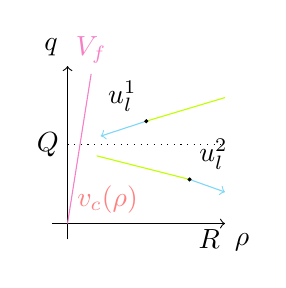
\begin{tikzpicture}
% coordinates
\draw[->] (0,-0.2) -- (0,2) node[anchor= south east] {$q$};
\draw[->] (-0.2,0) -- (2,0) node[anchor= north west] {$\rho$};
% rarefactions
\draw[<-][cyan!50] (0.42, 1.11) -- (1, 1.3) ;
\draw[lime] (1, 1.3) -- (2, 1.6) ;

\draw[->][cyan!50] (1.55,0.56)  -- (2, 0.4) ;
\draw[-][lime] (0.37, 0.86) -- (1.55,0.56)  ;


% v_c
\draw[red!50, domain=0:0.69]  plot[id=x] function{x*(3*x+1)}  node[anchor= south west] {$v_c(\rho)$};
% V_f
\draw[magenta!50] (0,0) -- (0.3, 1.9);
\node[magenta!50] at (0.3, 2.2) {$V_f$};

\draw[dotted] (0,1) -- (2, 1);

\filldraw[black] (1,1.3) circle (0.5pt) node[anchor = south east]{$u_l^1$} ;
\filldraw[black] (1.55,0.56) circle (0.5pt) node[anchor = south west]{$u_l^2$} ;
% contacts
\draw[ orange!50, domain=0:1.86]  plot[id=x] function{(x/1.38)*(2-1.38)/(2-x)*0.33};
\draw[ orange!50, domain=0:1.28]  plot[id=x] function{(x/1.16)*(2-1.16)/(2-x)*1.63};
%
%\node at (1, 1.55) {$u_l$};
\node at (1.8, -0.2) {$R$};
\node at (-0.25, 1) {$Q$};
\end{tikzpicture}
\caption{Wave solutions from two starting points $u_l^1$ and $u_l^2$. }
\label{Fig:FullSol_ic_rhoq}
\end{minipage}
\quad \quad \quad \quad 
\begin{minipage}{.35\textwidth}
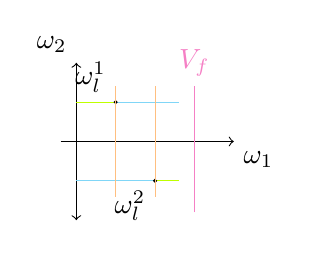
\begin{tikzpicture}
% coordinates
\draw[<->] (0,0) -- (0,2) node[anchor= south east] {$\omega_2$};
\draw[->] (-0.2,1) -- (2,1) node[anchor= north west] {$\omega_1$};
% rarefactions
% rarefactions
\draw[lime] (0, 1.5) -- (0.5, 1.5) ;
\draw[cyan!50] (0.5, 1.5) -- (1.3, 1.5)  ;
\filldraw[black] (0.5, 1.5) circle (0.5pt) node[anchor = south east]{$\omega_l^1$} ;

\draw[cyan!50] (0, 0.5) -- (1, 0.5) ;
\draw[lime] (1, 0.5) -- (1.3, 0.5) ;
\filldraw[black] (1, 0.5)  circle (0.5pt) node[anchor = north east]{$\omega_l^2$} ;

% contacts
\draw[orange!50] (0.5, 1.7) -- (0.5, 0.3) ;
\draw[orange!50] (1, 1.7) -- (1, 0.3) ;

% free ph line
\draw[magenta!50] (1.5, 0.1) -- (1.5, 1.7); 
\node[magenta!50] at (1.5, 2) {$V_f$};
%\filldraw[black] (1.5, 1.5)  circle (0.5pt) node[anchor =  west]{$\omega_r^2$} ;
%\filldraw[black] (1.5, 0.5)  circle (0.5pt) node[anchor = west]{$\omega_r^2$} ;

\end{tikzpicture}
\caption{Wave solutions from two starting points $\omega_l^1$ and $\omega_l^2$.}
\label{Fig:FullSol_ic_ww}
\end{minipage}
\end{figure}

% -----------------------------------------------------------
% -----------------------------------------------------------
% -----------------------------------------------------------
\begin{comment}

From Figure \ref{Fig:FullSol_ic_rhoq}, observe that
\begin{align*}
    q > Q \begin{cases}
    q \searrow rarefaction\\
    q \nearrow shock
    \end{cases}
    q < Q \begin{cases}
    q \searrow shock \\
    q \nearrow rarefaction
    \end{cases}
\end{align*}

Using the relation between the coordinates $\rho, q$ and $\omega_1, \omega_2$ 
\begin{itemize}
    \item $\omega_2 > 0$ 
    $\rho$ const. $q \searrow \leftrightarrow \omega_1, \omega_2 \searrow$ rarefaction
    \item $\omega_2 < 0$ 
    $\rho$ const. $q \searrow \leftrightarrow \omega_1, \omega_2 \searrow$ shock
\end{itemize}

Which means we have the relation between shock and rarefaction in $\omega$-coordinates, the result can be seen in Figure \ref{Fig:FullSol_ic_ww}
\begin{align*}
    \omega_2 > 0 \begin{cases}
    \omega_2 \searrow rarefaction\\
    \omega_2 \nearrow shock
    \end{cases}
    \omega_2 < 0\begin{cases}
    \omega_2 \searrow shock \\
    \omega_2 \nearrow rarefaction
    \end{cases}
\end{align*}
\end{comment}
% -----------------------------------------------------------
% -----------------------------------------------------------

\paragraph{Generalised Lax curves.}
We will first start by investigating the simplest case, where $u_l$ and $u_r$ lie on the same extension of the first wave curve. Let $ u_r \in W_1(u_l)$, and we draw the first family wave curve connecting $u_l$ and $u_r$. The different possibilities are stated below, and have corresponding figures to the right. We will first state the result, and then give a proof for the following case $1.$ and $2.$ at the end. We denote the rarefaction waves with blue, shock waves with green and phase transitions with yellow.  

\begin{enumerate}
\item $u_l \in \Omega_c$, $u_r \in \Omega_f$ \newline
\newline
  \begin{minipage}[t]{0.4\linewidth}
    \begin{enumerate}
    \item $q > Q:$ Starting in $u_l$ the solution is a rarefaction wave down to $u_m$ followed by a phase transition  from $u_m$ to $u_r$.
    \item $q < Q:$ Starting in $u_l$ the solution is a shock-like phase transition $u_r$.
    \item $q = Q:$ The solution is single phase-transition acting as a contact discontinuity.
    \end{enumerate}
  \end{minipage}
  \begin{minipage}[t]{0.5\linewidth}
    \centering
    \strut\vspace*{-\baselineskip}\newline\begin{minipage}{.3\textwidth}
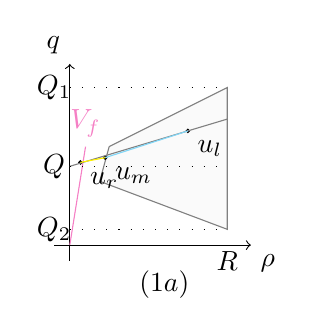
\begin{tikzpicture}
% coordinates
    \filldraw[fill=black!2, draw=black!50] plot [tension = 1] coordinates { (0.5,1.25) (2,2) (2,0.2) (0.38, 0.81) (0.5,1.25)};
    \draw[->] (0,-0.2) -- (0,2.3) node[anchor=south east] {$q$};
    %\draw[red!50, domain=0:0.7]  plot[id=x] function{x*(3*x+1)}  node[above] {$v_c(\rho)$};
    \draw[magenta!50] (0,0) -- (0.2,1.25) node[anchor = south] {$V_f$};
    %\node[magenta!50] at (0.3,2.5) {$V_f$};
    \filldraw[black] (0.135,1.05) circle (0.6pt) node[anchor = north west]{$u_r$} ;
    \filldraw[black] (0.45,1.11) circle (0.6pt) node[anchor = north west]{$u_m$} ;
    \filldraw[black] (1.5,1.45) circle (0.6pt) node[anchor = north west]{$u_l$} ;
    % \node at (1,1) {$\Omega_c$};
     \draw[->] (-0.2,0) -- (2.3,0) node[anchor=north west] {$\rho$};
     \draw[-][black!50] (0, 1) -- (2, 1.6) ;
    \node at (2,-0.2) {$R$};
     \node at (-0.2,2) {$Q_1$};
     \node at (-0.2,0.2) {$Q_2$};
     \node at (-0.2,1) {$Q$};
     \draw[loosely dotted] (0,1) -- (2,1);
     \draw[loosely dotted] (0,2) -- (2,2);
     \draw[loosely dotted] (0,0.2) -- (2,0.2);
     \node at (1.2,-0.5) {$(1a)$};
     % rarefactions and shocks
    %\draw[lime] (1.05, 1.33) -- (2, 1.6) ;
    %\draw[<-][cyan!50] (0.42, 1.19) -- (1, 1.33) ;
    
    %\draw[->][lime] (1.48,0.4)  -- (2, 0.2) ;
    \draw[-][cyan!50] (0.45,1.11) -- (1.5,1.45)  ;
    \draw[yellow] (0.135,1.05) -- (0.45,1.11);
    %middlepoints
     %\filldraw[black] (0.9, 0.6) circle (0.5pt) node[anchor = north]{$u_m$} ;
     %\filldraw[black] (1.48,0.4) circle (0.5pt) node[anchor =  west]{$u_r$} ;
    %endpoints
    %\filldraw[black] (1.05,1.33) circle (0.5pt) node[anchor = south east]{$u_r^1$} ;
    %\filldraw[black] (1.55,0.56) circle (0.5pt) node[anchor = south west]{$u_r^2$} ;
    
    % contacts
    %\draw[ orange!50, domain=0:1.86]  plot[id=x] function{(x/1.38)*(2-1.38)/(2-x)*0.33};
    %\draw[ orange!50, domain=0:1.28]  plot[id=x] function{(x/1.16)*(2-1.16)/(2-x)*1.63};
     
\end{tikzpicture}
\end{minipage}
\quad \quad \quad 
\begin{minipage}{.3\textwidth}
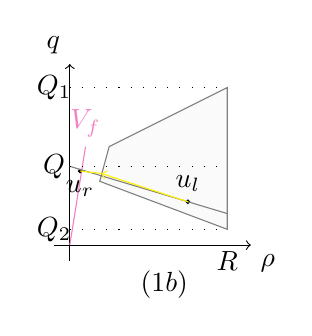
\begin{tikzpicture}
% coordinates
    \filldraw[fill=black!2, draw=black!50] plot [tension = 1] coordinates { (0.5,1.25) (2,2) (2,0.2) (0.38, 0.81) (0.5,1.25)};
    \draw[->] (0,-0.2) -- (0,2.3) node[anchor=south east] {$q$};
    %\draw[red!50, domain=0:0.7]  plot[id=x] function{x*(3*x+1)}  node[above] {$v_c(\rho)$};
    \draw[magenta!50] (0,0) -- (0.2,1.25) node[anchor = south] {$V_f$};
    %\node[magenta!50] at (0.3,2.5) {$V_f$};
    \filldraw[black] (0.13,0.94) circle (0.6pt) node[anchor = north]{$u_r$} ;
    \filldraw[black] (1.5,0.55) circle (0.6pt) node[anchor = south ]{$u_l$} ;
    %\filldraw[black] (0.4,0.91) circle (0.6pt) node[anchor = south west]{$u_m$} ;
    \draw[-][black!50] (0, 1) -- (2, 0.4) ;
    % \node at (1,1) {$\Omega_c$};
     \draw[->] (-0.2,0) -- (2.3,0) node[anchor=north west] {$\rho$};
    \node at (2,-0.2) {$R$};
     \node at (-0.2,2) {$Q_1$};
     \node at (-0.2,0.2) {$Q_2$};
     \node at (-0.2,1) {$Q$};
     \draw[loosely dotted] (0,1) -- (2,1);
     \draw[loosely dotted] (0,2) -- (2,2);
     \draw[loosely dotted] (0,0.2) -- (2,0.2);
     \node at (1.2,-0.5) {$(1b)$};
     % rarefactions and shocks
    %\draw[lime] (1.05, 1.33) -- (2, 1.6) ;
    %\draw[<-][cyan!50] (0.42, 1.19) -- (1, 1.33) ;
    
    \draw[->][yellow] (1.5,0.55)  -- (0.4,0.91) ;
    %\draw[-][cyan!50] (0.37, 0.83) -- (1.48,0.4)  ;
    \draw[yellow] (0.13,0.94) -- (0.4,0.91);
    %middlepoints
     %\filldraw[black] (0.9, 0.6) circle (0.5pt) node[anchor = north]{$u_m$} ;
     %\filldraw[black] (1.48,0.4) circle (0.5pt) node[anchor =  west]{$u_r$} ;
    %endpoints
    %\filldraw[black] (1.05,1.33) circle (0.5pt) node[anchor = south east]{$u_r^1$} ;
    %\filldraw[black] (1.55,0.56) circle (0.5pt) node[anchor = south west]{$u_r^2$} ;
    
    % contacts
    %\draw[ orange!50, domain=0:1.86]  plot[id=x] function{(x/1.38)*(2-1.38)/(2-x)*0.33};
    %\draw[ orange!50, domain=0:1.28]  plot[id=x] function{(x/1.16)*(2-1.16)/(2-x)*1.63};
     
\end{tikzpicture}
\end{minipage}
  \end{minipage}
\item $u_r \in \Omega_c$, $u_l \in \Omega_f$ \newline
\newline
  \begin{minipage}[t]{0.4\linewidth}
    \begin{enumerate}
    \item $q > Q:$ Starting in $u_l$ the solution is a shock-like phase transition to $u_r$.
    \item $q < Q:$ Starting in $u_l$ the solution is a phase transition to $u_m$ followed by a rarefaction wave from $u_m$ to $u_r$.
    \item $q = Q:$ The solution is single phase-transition acting as a contact discontinuity.
    \end{enumerate}
  \end{minipage}
  \begin{minipage}[t]{0.5\linewidth}
    \centering
    \strut\vspace*{-\baselineskip}\newline\begin{minipage}{.3\textwidth}
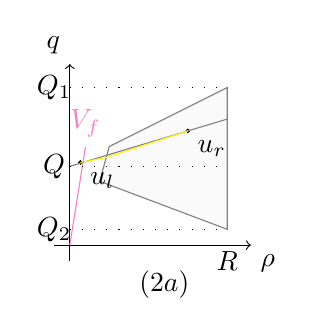
\begin{tikzpicture}
% coordinates
    \filldraw[fill=black!2, draw=black!50] plot [tension = 1] coordinates { (0.5,1.25) (2,2) (2,0.2) (0.38, 0.81) (0.5,1.25)};
    \draw[->] (0,-0.2) -- (0,2.3) node[anchor=south east] {$q$};
    %\draw[red!50, domain=0:0.7]  plot[id=x] function{x*(3*x+1)}  node[above] {$v_c(\rho)$};
    \draw[magenta!50] (0,0) -- (0.2,1.25) node[anchor = south] {$V_f$};
    %\node[magenta!50] at (0.3,2.5) {$V_f$};
    \filldraw[black] (0.135,1.05) circle (0.6pt) node[anchor = north west]{$u_l$} ;
    %\filldraw[black] (0.45,1.11) circle (0.6pt) node[anchor = north west]{$u_m$} ;
    \filldraw[black] (1.5,1.45) circle (0.6pt) node[anchor = north west]{$u_r$} ;
    % \node at (1,1) {$\Omega_c$};
     \draw[->] (-0.2,0) -- (2.3,0) node[anchor=north west] {$\rho$};
     \draw[-][black!50] (0, 1) -- (2, 1.6) ;
    \node at (2,-0.2) {$R$};
     \node at (-0.2,2) {$Q_1$};
     \node at (-0.2,0.2) {$Q_2$};
     \node at (-0.2,1) {$Q$};
     \draw[loosely dotted] (0,1) -- (2,1);
     \draw[loosely dotted] (0,2) -- (2,2);
     \draw[loosely dotted] (0,0.2) -- (2,0.2);
     \node at (1.2,-0.5) {$(2a)$};
     % rarefactions and shocks
    %\draw[lime] (1.05, 1.33) -- (2, 1.6) ;
    %\draw[<-][cyan!50] (0.42, 1.19) -- (1, 1.33) ;
    
    %\draw[->][lime] (1.48,0.4)  -- (2, 0.2) ;
    \draw[-][yellow] (0.45,1.11) -- (1.5,1.45)  ;
    \draw[yellow] (0.135,1.05) -- (0.45,1.11);
    %middlepoints
     %\filldraw[black] (0.9, 0.6) circle (0.5pt) node[anchor = north]{$u_m$} ;
     %\filldraw[black] (1.48,0.4) circle (0.5pt) node[anchor =  west]{$u_r$} ;
    %endpoints
    %\filldraw[black] (1.05,1.33) circle (0.5pt) node[anchor = south east]{$u_r^1$} ;
    %\filldraw[black] (1.55,0.56) circle (0.5pt) node[anchor = south west]{$u_r^2$} ;
    
    % contacts
    %\draw[ orange!50, domain=0:1.86]  plot[id=x] function{(x/1.38)*(2-1.38)/(2-x)*0.33};
    %\draw[ orange!50, domain=0:1.28]  plot[id=x] function{(x/1.16)*(2-1.16)/(2-x)*1.63};
     
\end{tikzpicture}
\end{minipage}
\quad \quad \quad 
\begin{minipage}{.3\textwidth}
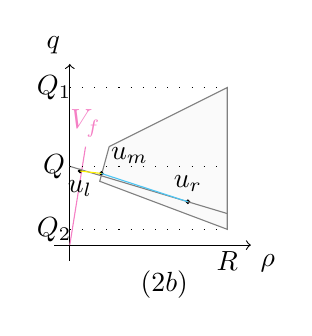
\begin{tikzpicture}
% coordinates
    \filldraw[fill=black!2, draw=black!50] plot [tension = 1] coordinates { (0.5,1.25) (2,2) (2,0.2) (0.38, 0.81) (0.5,1.25)};
    \draw[->] (0,-0.2) -- (0,2.3) node[anchor=south east] {$q$};
    %\draw[red!50, domain=0:0.7]  plot[id=x] function{x*(3*x+1)}  node[above] {$v_c(\rho)$};
    \draw[magenta!50] (0,0) -- (0.2,1.25) node[anchor = south] {$V_f$};
    %\node[magenta!50] at (0.3,2.5) {$V_f$};
    \filldraw[black] (0.13,0.94) circle (0.6pt) node[anchor = north]{$u_l$} ;
    \filldraw[black] (1.5,0.55) circle (0.6pt) node[anchor = south ]{$u_r$} ;
    \filldraw[black] (0.4,0.91) circle (0.6pt) node[anchor = south west]{$u_m$} ;
    \draw[-][black!50] (0, 1) -- (2, 0.4) ;
    % \node at (1,1) {$\Omega_c$};
     \draw[->] (-0.2,0) -- (2.3,0) node[anchor=north west] {$\rho$};
    \node at (2,-0.2) {$R$};
     \node at (-0.2,2) {$Q_1$};
     \node at (-0.2,0.2) {$Q_2$};
     \node at (-0.2,1) {$Q$};
     \draw[loosely dotted] (0,1) -- (2,1);
     \draw[loosely dotted] (0,2) -- (2,2);
     \draw[loosely dotted] (0,0.2) -- (2,0.2);
     \node at (1.2,-0.5) {$(2b)$};
     % rarefactions and shocks
    %\draw[lime] (1.05, 1.33) -- (2, 1.6) ;
    %\draw[<-][cyan!50] (0.42, 1.19) -- (1, 1.33) ;
    
    \draw[-][cyan!70] (1.5,0.55)  -- (0.4,0.91) ;
    %\draw[-][cyan!50] (0.37, 0.83) -- (1.48,0.4)  ;
    \draw[yellow] (0.13,0.94) -- (0.4,0.91);
    %middlepoints
     %\filldraw[black] (0.9, 0.6) circle (0.5pt) node[anchor = north]{$u_m$} ;
     %\filldraw[black] (1.48,0.4) circle (0.5pt) node[anchor =  west]{$u_r$} ;
    %endpoints
    %\filldraw[black] (1.05,1.33) circle (0.5pt) node[anchor = south east]{$u_r^1$} ;
    %\filldraw[black] (1.55,0.56) circle (0.5pt) node[anchor = south west]{$u_r^2$} ;
    
    % contacts
    %\draw[ orange!50, domain=0:1.86]  plot[id=x] function{(x/1.38)*(2-1.38)/(2-x)*0.33};
    %\draw[ orange!50, domain=0:1.28]  plot[id=x] function{(x/1.16)*(2-1.16)/(2-x)*1.63};
     
\end{tikzpicture}
\end{minipage}
  \end{minipage}
  

A priori one might expect $1b)$ and $2a)$ to produce in the first case a $1$-shock and then a shock-like phase transition, and in the last case a phase transition followed by a $1$-shock. We will now prove why this is not the case, and the correct order of $\lambda_1$ and $\Lambda$. 
\begin{equation}
    \Lambda(\rho) = \frac{\rho_l v_l - \rho v_c(\rho, q_m(\rho))}{\rho_l - \rho}.
    \label{Eq:PhaseBoundarySpeed}
\end{equation}
Recall that the speed of the phase boundary is assigned by the Rankine-Hugoniot condition for phase transitions (\ref{Eq:RH_PhT}), and has the speed (\ref{Eq:PhaseBoundarySpeed}). Let $\rho_i$ be the density corresponding to the points $u_i$. For case $1.$ to fulfil (\ref{Eq:APrioriCongToFree}) we have the entropy requirement 
\begin{align*}
    \lambda_1(u_l) < \lambda_1(u_m) < \Lambda(u_m) = \lambda(u_r).
\end{align*}
We investigate when $\lambda_1(u_m) = \Lambda(u_m)$, and note that $0 < \rho_r < \rho_m < \rho_l$
\begin{align*}
    (\frac{2}{R} - \frac{1}{\rho_m})(q_m -Q) - \frac{Q}{R} = \frac{\rho_m v_c(\rho_m) - \rho_r v_f(\rho_r)}{\rho_m - \rho_r}.
    %\label{Eq:stepLambdas}
\end{align*}
After tedious computation we end up with
\begin{align}
    %\lambda_1(u_m) &= \Lambda(u_m), \nonumber \\
    3\rho_m - 2\rho_r &= \frac{\rho_r^2 V + R(2q_m -Q)}{q_m -Q}.
    \label{Eq:ConditionOnLambdas}
\end{align}
This also holds for case $2.$, we simply replace $\rho_r$ by $\rho_l$ in the steps taken above.
In the case $1b)$ and $1c)$ we have $q_m - Q < 0 $ which make the right hand side of (\ref{Eq:ConditionOnLambdas}) negative, and the left hand side is positive as $\rho_m > \rho_r$ in case $1.$ and $\rho_m > \rho_l$ in case $2$. This implies that in the point $u_m$ we have 
\begin{equation*}
  q < Q: \quad \lambda_1(u_m) > \Lambda(u_m)
\end{equation*}
This prohibits a $1$-shock from $u_l$ to $u_m $ in the case of $q < Q$. And thus we have a single shock-like phase transition from $u_l$ to $u_r$ in $1b)$. In the case of $2b)$ the wave speeds are well ordered, and we allow for both a phase transition and a rarefaction coming from the left. Furthermore, when $Q = q_m = q_l$ and he first family wave is a contact in both cases $\lambda_1(u_m) = \Lambda(u_m)$ and the result will be a single phase-transition acting as a contact discontinuity. 
For the case when $q > Q$ we need some more analysis of (\ref{Eq:ConditionOnLambdas}), and another requirement. For now, we can say that the denominator in (\ref{Eq:ConditionOnLambdas}) will be quite small, so the right hand side will be a lot larger than the left. We can also say that left hand side will never be larger than $3R$, and if that is the worst case scenario we require $q_m = 2Q$. This is a crude approximation, but insightful to some extent. Thus we have
\begin{equation*}
  q > Q:  \quad \lambda_1(u_m) < \Lambda(u_m)
\end{equation*}
proving the cases $1.$ and $2.$ above.

Now we will investigate what happens when we are below the extension of the lower first wave curve. Let $q_m(\rho) = Q + \rho/R(Q_2 - Q)$ be this lower boundary wave curve, and for simplicity let $u_r \in q_m(\rho)$.
In order to determine which behaviour we will see when travelling from one phase to the other we define the following. As in \cite{Colombo2002}, let $\check R_c$ be the smallest density on $q_m(\rho) \in \Omega_c$. We first state the result, and give a proof at the end. 

\item $u_l \in \Omega_f$, $u_r \in \Omega_c$ 
    \begin{enumerate}
    \item $\Lambda(\check R) \leq \lambda(\check R)$ then the solution will be a phase transition from $u_l$ to $u_{m}$, followed by a rarefaction wave $w_1$ to $u_r$. 
    \item Somewhere on the line $q_m$ there is a density $\rho_m$ where $\Lambda(\rho)$ goes from being larger than $\lambda_1(\rho)$ to being equal and then to be smaller than $\lambda_1(\rho)$. This point will be $u_{m}$ and in this case we have a compound wave composed by a phase-transition, and attached to it a rarefaction wave $w_1$. 
    \item $ \Lambda( \rho) > \lambda(\rho)$, for $\check R < \rho < \rho_r$, then we will not have a middle state $u_{m}$ and will travel straight to $u_r$ on a shock-like phase transition.
    \end{enumerate}
\begin{figure}[H]
    \centering
    \begin{minipage}{.3\textwidth}
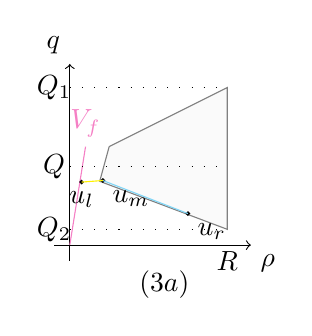
\begin{tikzpicture}
% coordinates
    \filldraw[fill=black!2, draw=black!50] plot [tension = 1] coordinates { (0.5,1.25) (2,2) (2,0.2) (0.38, 0.81) (0.5,1.25)};
    \draw[->] (0,-0.2) -- (0,2.3) node[anchor=south east] {$q$};
   
    \draw[magenta!50] (0,0) -- (0.2,1.25) node[anchor = south] {$V_f$};
    
    \filldraw[black] (1.5,0.4) circle (0.6pt) node[anchor = north west]{$u_r$} ;
    \filldraw[black] (0.42,0.82) circle (0.6pt) node[anchor = north west]{$u_m$} ;
    \filldraw[black] (0.15,0.8) circle (0.6pt) node[anchor = north]{$u_l$} ;
    % \node at (1,1) {$\Omega_c$};
     \draw[->] (-0.2,0) -- (2.3,0) node[anchor=north west] {$\rho$};
    % \draw[-][black!50] (0, 0.98) -- (2, 0.2) node[anchor=south west] {$q_m(\rho)$} ;
    \node at (2,-0.2) {$R$};
     \node at (-0.2,2) {$Q_1$};
     \node at (-0.2,0.2) {$Q_2$};
     \node at (-0.2,1) {$Q$};
     \draw[loosely dotted] (0,1) -- (2,1);
     \draw[loosely dotted] (0,2) -- (2,2);
     \draw[loosely dotted] (0,0.2) -- (2,0.2);
     \node at (1.2,-0.5) {$(3a)$};
     % rarefactions and shocks
    %\draw[lime] (1.05, 1.33) -- (2, 1.6) ;
    %\draw[<-][cyan!50] (0.42, 1.19) -- (1, 1.33) ;
    
    %\draw[->][lime] (1.48,0.4)  -- (2, 0.2) ;
    \draw[cyan!50] (0.42,0.82) -- (1.5,0.4)  ;
    \draw[yellow] (0.15,0.8) -- (0.42,0.82);
     
\end{tikzpicture}
\end{minipage}
\begin{minipage}{.3\textwidth}
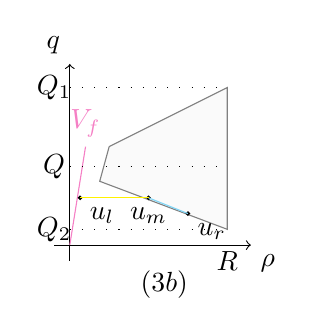
\begin{tikzpicture}
% coordinates
    \filldraw[fill=black!2, draw=black!50] plot [tension = 1] coordinates { (0.5,1.25) (2,2) (2,0.2) (0.38, 0.81) (0.5,1.25)};
    \draw[->] (0,-0.2) -- (0,2.3) node[anchor=south east] {$q$};
   
    \draw[magenta!50] (0,0) -- (0.2,1.25) node[anchor = south] {$V_f$};
    
    \filldraw[black] (1.5,0.4) circle (0.6pt) node[anchor = north west]{$u_r$} ;
    \filldraw[black] (1,0.6) circle (0.6pt) node[anchor = north]{$u_m$} ;
    \filldraw[black] (0.13,0.6) circle (0.6pt) node[anchor = north west]{$u_l$} ;
    % \node at (1,1) {$\Omega_c$};
     \draw[->] (-0.2,0) -- (2.3,0) node[anchor=north west] {$\rho$};
    % \draw[-][black!50] (0, 0.98) -- (2, 0.2) node[anchor=south west] {$q_m(\rho)$} ;
    \node at (2,-0.2) {$R$};
     \node at (-0.2,2) {$Q_1$};
     \node at (-0.2,0.2) {$Q_2$};
     \node at (-0.2,1) {$Q$};
     \draw[loosely dotted] (0,1) -- (2,1);
     \draw[loosely dotted] (0,2) -- (2,2);
     \draw[loosely dotted] (0,0.2) -- (2,0.2);
     \node at (1.2,-0.5) {$(3b)$};
     % rarefactions and shocks
    %\draw[lime] (1.05, 1.33) -- (2, 1.6) ;
    %\draw[<-][cyan!50] (0.42, 1.19) -- (1, 1.33) ;
    
    %\draw[->][lime] (1.48,0.4)  -- (2, 0.2) ;
    \draw[-][cyan!50] (1,0.6) -- (1.5,0.4)  ;
    \draw[yellow] (0.13,0.6) -- (1,0.6);
     
\end{tikzpicture}
\end{minipage}
\begin{minipage}{.3\textwidth}
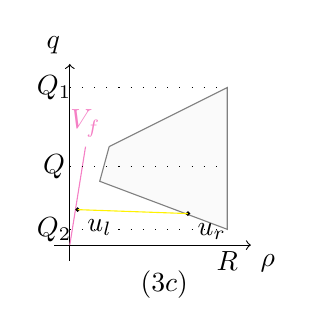
\begin{tikzpicture}
% coordinates
    \filldraw[fill=black!2, draw=black!50] plot [tension = 1] coordinates { (0.5,1.25) (2,2) (2,0.2) (0.38, 0.81) (0.5,1.25)};
    \draw[->] (0,-0.2) -- (0,2.3) node[anchor=south east] {$q$};
   
    \draw[magenta!50] (0,0) -- (0.2,1.25) node[anchor = south] {$V_f$};
    
    \filldraw[black] (1.5,0.4) circle (0.6pt) node[anchor = north west]{$u_r$} ;
    %\filldraw[black] (0.42,0.82) circle (0.6pt) node[anchor = north west]{$u_m$} ;
    \filldraw[black] (0.1,0.45) circle (0.6pt) node[anchor = north west]{$u_l$} ;
    % \node at (1,1) {$\Omega_c$};
     \draw[->] (-0.2,0) -- (2.3,0) node[anchor=north west] {$\rho$};
    % \draw[-][black!50] (0, 0.98) -- (2, 0.2) node[anchor=south west] {$q_m(\rho)$} ;
    \node at (2,-0.2) {$R$};
     \node at (-0.2,2) {$Q_1$};
     \node at (-0.2,0.2) {$Q_2$};
     \node at (-0.2,1) {$Q$};
     \draw[loosely dotted] (0,1) -- (2,1);
     \draw[loosely dotted] (0,2) -- (2,2);
     \draw[loosely dotted] (0,0.2) -- (2,0.2);
     \node at (1.2,-0.5) {$(3c)$};
     % rarefactions and shocks
    %\draw[lime] (1.05, 1.33) -- (2, 1.6) ;
    %\draw[<-][cyan!50] (0.42, 1.19) -- (1, 1.33) ;
    
    %\draw[->][lime] (1.48,0.4)  -- (2, 0.2) ;
    %\draw[-][cyan!50] (0.45,1.11) -- (1.5,1.45)  ;
    \draw[yellow] (0.1,0.45) -- (1.5,0.4);
     
\end{tikzpicture}
\end{minipage}

    \caption{Corresponding solutions in the $(\rho, q)$-plane for case $3.$}
    \label{fig:PhTComplexCase1}
\end{figure}
 
\item $u_l \in \Omega_c$, $u_r \in \Omega_f$ \newline
     $ \Lambda( \rho) < \lambda(\rho)$, for $\check R < \rho < \rho_r$, then we will not have a middle state $u_{m_1}$ and will travel straight to $u_r$ on a shock-like phase transition.
\end{enumerate}

The argument for case $1.$ and $2.$ still holds for case $3.,$ and $4.$ . However, as the phase boundary may hit the congested phase for a larger $\rho$ than in the previous cases, we cannot guarantee that we first see a phase transition with speed $\Lambda$ followed by a first family wave $\lambda$, as in case $2b)$. Thus in case $3.$ we will have three scenarios, where one might be a composite wave. This compound wave is similar to what we see in scalar cases when using convex envelopes. We get a part where the speed is not growing $\Lambda(u_l)$ to $\Lambda(u_m)$, and the place where the two speeds match, at $\Lambda(u_m) = \lambda_1(u_m)$, we reconnect to he original flux function, in the case of the convex envelope, and continue along that path.  In $4.$, going from $u_l \in \Omega_c$ to $\Omega_f$ we get the same result as in $1b)$ a single phase transition acting as a shock. For case $4.$ we use the argument from $1b)$, and see that in this case we only have one possible solution.
   
In the $(x,t)$-plane we have the following waves shown in Figure \ref{fig:PhTSolInXT}. The left shows the cases $1a)$ and $3a)$, and also the case $2b)$ if one reverts the $x$-axis and letting the phase-transition come first. The middle shows the cases $1b), 2a) \text{and} 3c)$. Where as the only instance we have a compound wave, the right figure is the case of $3b)$. 
\begin{figure}
    \centering
    \begin{minipage}{.3\textwidth}
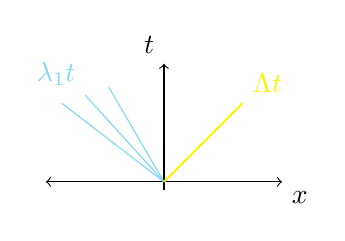
\begin{tikzpicture}
% coord.
\draw[<->] (-1.5,0) -- (1.5,0) node[anchor= north west] {$x$};
\draw[->] (0,-0.1) -- (0,1.5) node[anchor=south east] {$t$};
% contact disc
\draw[color=yellow, line width=0.25mm] (0,0) -- (1,1) node[anchor= south west] {$\Lambda t$};
% rarefaction
\draw[color=cyan!50!white] (0,0) -- (-1.3,1);
\draw[color=cyan!50!white] (0,0) -- (-1,1.1) node[anchor= south east] {$\lambda_1 t$};
\draw[color=cyan!50!white] (0,0) -- (-0.7,1.2);
%\node at (1.2,-0.5) {$(3a)$};
\end{tikzpicture}
%\caption{Slow rarefaction (blue) followed by a phase transition (yellow).}
%\label{Fig:SolRPRarefactionDiscCongestedPhase}
\end{minipage}
\quad 
\begin{minipage}{.3\textwidth}
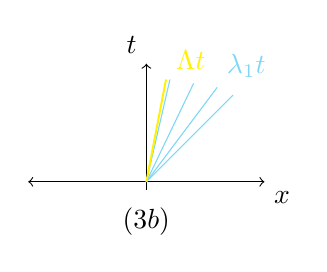
\begin{tikzpicture}
\draw[<->] (-1.5,0) -- (1.5,0) node[anchor= north west] {$x$};
\draw[->] (0,-0.1) -- (0,1.5) node[anchor=south east] {$t$};

\draw[color=cyan!50!white] (0,0) -- (1.1,1.1);
\draw[color=cyan!50!white] (0,0) -- (0.9,1.2) node[anchor= south west] {$\lambda_1 t$};
\draw[color=cyan!50!white] (0,0) -- (0.6,1.25);
\draw[color=cyan!50!white] (0,0) -- (0.3,1.3);
\draw[color=yellow, line width=0.25mm] (0,0) -- (0.25,1.3) node[anchor= south west] {$\Lambda t$};
\node at (0,-0.5) {$(3b)$};
\end{tikzpicture}
%\caption{Contact discontinuity followed by a contact discontinuity, $q_l = Q$.}
%\label{Fig: SolRPDiscCongestedPhase}
\end{minipage}
\quad 
\begin{minipage}{.3\textwidth}
\begin{tikzpicture}
\draw[<->] (-1.5,0) -- (1.5,0) node[anchor= north west] {$x$};
\draw[->] (0,-0.1) -- (0,1.5) node[anchor=south east] {$t$};
\draw[color=yellow, line width=0.25mm] (0,0) -- (1,1) node[anchor= south west] {$\Lambda t$};
%\draw[color=lime] (0,0) -- (-1,1) node[anchor= south east] {$\lambda_1 t$};
%\node at (1.2,-0.5) {$(3c)$};
\end{tikzpicture}
%\caption{A single phase transition (yellow) acting as a shock or contact.}
%\label{Fig: SolRPShockDiskCongestedPhase}
\end{minipage}


    \caption{\textit{Left:} Slow rarefaction (blue) followed by a phase transition (yellow). \textit{Middle:} A single phase transition (yellow) acting as a shock or contact. \textit{Right:} Contact discontinuity followed by a contact discontinuity, $q_l = Q$.}
    \label{fig:PhTSolInXT}
\end{figure}
We can now state the solutions above for $u(x,t)$.
\begin{align}
    u_{1a}(x,t) = \begin{cases}
        u_l & \text{ for $ x < \lambda_1(u_r)t$}, \\
         w_1 &\text{ for $  \lambda_1(u_l)t < x < \lambda_1(u_m)$}, \\
        u_m & \text{ for $  \lambda_1(u_m)t < x < \Lambda(u_m)$}, \\
        u_r & \text{ for $x > \Lambda(u_r)t$},
    \end{cases} 
    \quad \quad 
    u_{1b}(x,t) = \begin{cases}
        u_l & \text{ for $ x < \Lambda(u_l)t$}, \\
        u_r & \text{ for $x > \Lambda( u_r)t$},
    \end{cases} 
    \label{Eq:Sol1}
\end{align}
\begin{align}
    u_{2a}(x,t) = \begin{cases}
        u_l & \text{ for $ x < \Lambda(u_l)t$}, \\
        u_r & \text{ for $x > \Lambda( u_r)t$},
    \end{cases} 
    \quad \quad 
    u_{2b}(x,t) = \begin{cases}
        u_l & \text{ for $ x < \Lambda(u_l)t$}, \\
        u_m & \text{ for $  \Lambda(u_m)t < x < \lambda_1(u_m)$}, \\
        w_1 &\text{ for $  \lambda_1(u_m)t < x < \lambda_1(u_r)$}, \\
        u_r & \text{ for $x > \lambda_1( u_r)t$},
    \end{cases} 
    \label{Eq:Sol2}
\end{align}

Looking back at one of the requiremens for the full model, was that we would nit allow this solution by any $2 \times 2$-system of conservayion laws. This follows the presence of $3$ waves in our solution. 

\begin{comment}

\begin{figure} \centering 
\begin{minipage}{.35\textwidth}
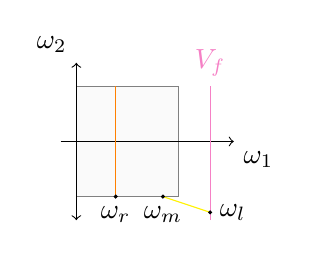
\begin{tikzpicture}
% coordinates
% Omega_c
\filldraw[fill=black!2, draw=black!50] plot [tension = 1] coordinates { (0,1.7) (1.3,1.7) (1.3,0.3) (0, 0.3) };
\draw[<->] (0,0) -- (0,2) node[anchor= south east] {$\omega_2$};
\draw[->] (-0.2,1) -- (2,1) node[anchor= north west] {$\omega_1$};
% rarefactions
%\draw[cyan!50] (0, 1.5) -- (0.5, 1.5) ;

%\draw[cyan] (0.5, 1.5) -- (1.3, 1.5)  ;
%\filldraw[black] (0.5, 1.5) circle (0.5pt) node[anchor = south east]{$\omega_r^1$} ;

%\draw[lime] (0, 0.5) -- (1, 0.5) ;
%\draw[line width=0.25mm,lime] (1, 0.7) -- (1.3, 0.7) ;
%\filldraw[black] (1, 0.7)  circle (0.5pt) node[anchor = east]{$\omega_r^2$} ;

% contacts
\draw[orange] (0.5, 1.7) -- (0.5, 0.3) ;
%\draw[orange] (1, 1.7) -- (1, 0.3) ;
\draw[yellow] (1.7, 0.1) -- (1.1, 0.3);

% free ph line
\draw[magenta!50] (1.7, 0) -- (1.7, 1.7); 
\node[magenta!50] at (1.7, 2) {$V_f$};
%\filldraw[black] (1.3, 0.3)  circle (0.5pt) node[anchor = north]{$\hat \omega$} ;
\filldraw[black] (1.1, 0.3)  circle (0.5pt) node[anchor = north]{$\omega_m$} ;
\filldraw[black] (0.5, 0.3)  circle (0.5pt) node[anchor = north]{$\omega_r$} ;
\filldraw[black] (1.7, 0.1)  circle (0.5pt) node[anchor = west]{$\omega_l$} ;
\end{tikzpicture}
\caption{The point $\omega_l$ below the lower boundary wave curve}
\label{Fig:solPhTransOutsidedomainOmega1}
\end{minipage}
\quad \quad \quad \quad 
\begin{minipage}{.35\textwidth}
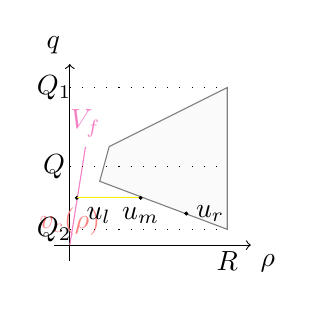
\begin{tikzpicture}
% coordinates
    \filldraw[fill=black!2, draw=black!50] plot [tension = 1] coordinates { (0.5,1.25) (2,2) (2,0.2) (0.38, 0.81) (0.5,1.25)};
    \draw[->] (0,-0.2) -- (0,2.3) node[anchor=south east] {$q$};
    \draw[red!50, domain=0:0.7]  plot[id=x] function{x*(3*x+1)}  node[above] {$v_c(\rho)$};
    \draw[magenta!50] (0,0) -- (0.2,1.25) node[anchor = south] {$V_f$};
    %\node[magenta!50] at (0.3,2.5) {$V_f$};
    \filldraw[black] (0.09,0.6) circle (0.5pt) node[anchor = north west]{$u_l$} ;
    % \node at (1,1) {$\Omega_c$};
     \draw[->] (-0.2,0) -- (2.3,0) node[anchor=north west] {$\rho$};
    \node at (2,-0.2) {$R$};
     \node at (-0.2,2) {$Q_1$};
     \node at (-0.2,0.2) {$Q_2$};
     \node at (-0.2,1) {$Q$};
     \draw[loosely dotted] (0,1) -- (2,1);
     \draw[loosely dotted] (0,2) -- (2,2);
     \draw[loosely dotted] (0,0.2) -- (2,0.2);
     % rarefactions and shocks
    %\draw[lime] (1.05, 1.33) -- (2, 1.6) ;
    %\draw[<-][cyan!50] (0.42, 1.19) -- (1, 1.33) ;
    
    %\draw[->][lime] (1.48,0.4)  -- (2, 0.2) ;
    %\draw[-][cyan!50] (0.37, 0.83) -- (1.48,0.4)  ;
    \draw[yellow] (0.09,0.6) -- (0.9, 0.6);
    %middlepoints
     \filldraw[black] (0.9, 0.6) circle (0.5pt) node[anchor = north]{$u_m$} ;
     \filldraw[black] (1.48,0.4) circle (0.5pt) node[anchor =  west]{$u_r$} ;
    %endpoints
    %\filldraw[black] (1.05,1.33) circle (0.5pt) node[anchor = south east]{$u_r^1$} ;
    %\filldraw[black] (1.55,0.56) circle (0.5pt) node[anchor = south west]{$u_r^2$} ;
    % contacts
    \draw[ orange!50, domain=0:1.86]  plot[id=x] function{(x/1.38)*(2-1.38)/(2-x)*0.33};
    %\draw[ orange!50, domain=0:1.28]  plot[id=x] function{(x/1.16)*(2-1.16)/(2-x)*1.63};
     
\end{tikzpicture}
\caption{$u_l$ below the lower boundary wave curve }
\label{Fig:Fig:solPhTransOutsidedomainRhoQ1}
\end{minipage}
\end{figure}
\end{comment}

%\caption{Wave solutions from two starting points $\omega_l^3$ and $\omega_l^3$.}
%\label{Fig:FullSol_ic_ww3}
%\end{wrapfigure}

\begin{comment}

\begin{figure} \centering 
\begin{minipage}{.35\textwidth}
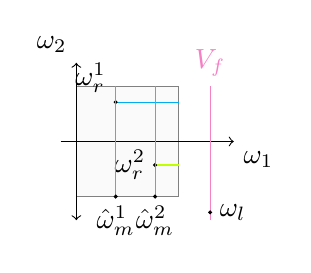
\begin{tikzpicture}
% coordinates
% Omega_c
\filldraw[fill=black!2, draw=black!50] plot [tension = 1] coordinates { (0,1.7) (1.3,1.7) (1.3,0.3) (0, 0.3) };
\draw[<->] (0,0) -- (0,2) node[anchor= south east] {$\omega_2$};
\draw[->] (-0.2,1) -- (2,1) node[anchor= north west] {$\omega_1$};
% rarefactions
%\draw[cyan!50] (0, 1.5) -- (0.5, 1.5) ;

\draw[cyan] (0.5, 1.5) -- (1.3, 1.5)  ;
\filldraw[black] (0.5, 1.5) circle (0.5pt) node[anchor = south east]{$\omega_r^1$} ;

%\draw[lime] (0, 0.5) -- (1, 0.5) ;
\draw[line width=0.25mm,lime] (1, 0.7) -- (1.3, 0.7) ;
\filldraw[black] (1, 0.7)  circle (0.5pt) node[anchor = east]{$\omega_r^2$} ;

% contacts
\draw[orange] (0.5, 1.7) -- (0.5, 0.3) ;
\draw[orange] (1, 1.7) -- (1, 0.3) ;

% free ph line
\draw[magenta!50] (1.7, 0) -- (1.7, 1.7); 
\node[magenta!50] at (1.7, 2) {$V_f$};
%\filldraw[black] (1.3, 0.3)  circle (0.5pt) node[anchor = north]{$\hat \omega$} ;
\filldraw[black] (1, 0.3)  circle (0.5pt) node[anchor = north]{$\hat \omega_m^2$} ;
\filldraw[black] (0.5, 0.3)  circle (0.5pt) node[anchor = north]{$\hat \omega_m^1$} ;
\filldraw[black] (1.7, 0.1)  circle (0.5pt) node[anchor = west]{$\omega_l$} ;
\end{tikzpicture}
\caption{The point $\omega_l$ below the lower boundary wave curve}
\label{Fig:solPhTransOutsidedomainOmega2}
\end{minipage}
\quad \quad \quad \quad 
\begin{minipage}{.35\textwidth}
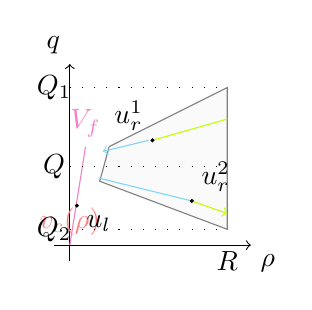
\begin{tikzpicture}
% coordinates
    \filldraw[fill=black!2, draw=black!50] plot [tension = 1] coordinates { (0.5,1.25) (2,2) (2,0.2) (0.38, 0.81) (0.5,1.25)};
    \draw[->] (0,-0.2) -- (0,2.3) node[anchor=south east] {$q$};
    \draw[red!50, domain=0:0.7]  plot[id=x] function{x*(3*x+1)}  node[above] {$v_c(\rho)$};
    \draw[magenta!50] (0,0) -- (0.2,1.25) node[anchor = south] {$V_f$};
    %\node[magenta!50] at (0.3,2.5) {$V_f$};
    \filldraw[black] (0.09,0.5) circle (0.5pt) node[anchor = north west]{$u_l$} ;
    % \node at (1,1) {$\Omega_c$};
     \draw[->] (-0.2,0) -- (2.3,0) node[anchor=north west] {$\rho$};
    \node at (2,-0.2) {$R$};
     \node at (-0.2,2) {$Q_1$};
     \node at (-0.2,0.2) {$Q_2$};
     \node at (-0.2,1) {$Q$};
     \draw[loosely dotted] (0,1) -- (2,1);
     \draw[loosely dotted] (0,2) -- (2,2);
     \draw[loosely dotted] (0,0.2) -- (2,0.2);
     % rarefactions and shocks
    \draw[lime] (1.05, 1.33) -- (2, 1.6) ;
    \draw[<-][cyan!50] (0.42, 1.19) -- (1, 1.33) ;
    
    \draw[->][lime] (1.55,0.56)  -- (2, 0.4) ;
    \draw[-][cyan!50] (0.37, 0.85) -- (1.55,0.56)  ;
    %middlepoints
     %\filldraw[black] (0.78, 0.68) circle (0.5pt) node[anchor = north]{$u_m^1$} ;
     %\filldraw[black] (1.55,0.56) circle (0.5pt) node[anchor =  west]{$u_m^2$} ;
    %endpoints
    \filldraw[black] (1.05,1.33) circle (0.5pt) node[anchor = south east]{$u_r^1$} ;
    \filldraw[black] (1.55,0.56) circle (0.5pt) node[anchor = south west]{$u_r^2$} ;
    % contacts
    \draw[ orange!50, domain=0:1.86]  plot[id=x] function{(x/1.38)*(2-1.38)/(2-x)*0.33};
    \draw[ orange!50, domain=0:1.28]  plot[id=x] function{(x/1.16)*(2-1.16)/(2-x)*1.63};
     
\end{tikzpicture}
\caption{$u_l$ below the lower boundary wave curve }
\label{Fig:Fig:solPhTransOutsidedomainRhoQ2}
\end{minipage}
\end{figure}


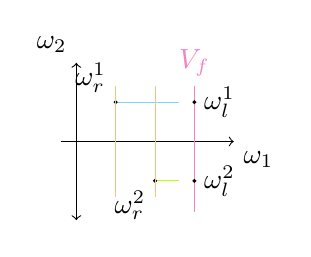
\begin{tikzpicture} %[scale=0.8, every node/.style={transform shape}]
% coordinates
\draw[<->] (0,0) -- (0,2) node[anchor= south east] {$\omega_2$};
\draw[->] (-0.2,1) -- (2,1) node[anchor= north west] {$\omega_1$};
% rarefactions
%\draw[cyan!50] (0, 1.5) -- (0.5, 1.5) ;
\draw[cyan!50] (0.5, 1.5) -- (1.3, 1.5)  ;
\filldraw[black] (0.5, 1.5) circle (0.5pt) node[anchor = south east]{$\omega_r^1$} ;

%\draw[lime] (0, 0.5) -- (1, 0.5) ;
\draw[lime] (1, 0.5) -- (1.3, 0.5) ;
\filldraw[black] (1, 0.5)  circle (0.5pt) node[anchor = north east]{$\omega_r^2$} ;

% contacts
\draw[orange!50] (0.5, 1.7) -- (0.5, 0.3) ;
\draw[orange!50] (1, 1.7) -- (1, 0.3) ;

% free ph line
\draw[magenta!50] (1.5, 0.1) -- (1.5, 1.7); 
\node[magenta!50] at (1.5, 2) {$V_f$};
\filldraw[black] (1.5, 1.5)  circle (0.5pt) node[anchor =  west]{$\omega_l^1$} ;
\filldraw[black] (1.5, 0.5)  circle (0.5pt) node[anchor = west]{$\omega_l^2$} ;
\end{tikzpicture}
\end{comment}

\newpage

\section{Qualitative properties}
Colombo proved the Cauchy problem admits a global solution in time, and without any assumptions on the number of phase boundaries or the smallness of initial data. In the proof of the Cauchy problem, the main tool is wave front-tracking, and it is shown that the model admits a bounded variation weak solution, and it holds globally for all times. Furthermore, global well-posedness for conservation laws developing phase transitions was shown by \cite{ColomboGoatinPriuli} in $2007$, using standards Riemann semigroups. 
Also qualitative properties from traffic flow were shown to agree with the properties of our model \cite{Colombo2003}.   

\textcolor{red}{This Riemann solver enjoys properties underlined in literature, se Colobo sine kilder. 2, 11, as not satisfied in several common models.}


One can reach a queue or a stop sign from anywhere in $\Omega_f$, even if in 80sone or in 40 sone. So it doesn't make sense to move from $u_l$ below $q_m$ up to the shortest distance between the two phases in order to do a phase transition. 


\newpage

\appendix
\section{Appendix}

\begin{theorem}[Divergence theorem]
Suppose $\Omega \subset \mathbb{R}$ with piecewise $C^1$ boundary $\partial \Omega$. For a vector field $F \in C^1(\bar \Omega; \mathbb{R}^n)$, 
\begin{equation}
    \int_\Omega \nabla \cdot F d^nx = \int_{\partial \Omega} F \cdot \vec{n} ds
\end{equation}
where $\vec{n} $ is the outward unit normal to $\partial \Omega$.
\label{Thm:Divergence}
\end{theorem}
A proof of this theorem (\ref{Thm:Divergence}) can be found in advanced calculus texts. 


\newpage
\printbibliography

\end{document}


